\documentclass[12pt,a4paper,openright]{report}

%\\usepackage\{url,graphicx\}\
\usepackage[pdftex]{graphicx}
\usepackage[bookmarks,%
            a4paper,%
            breaklinks,%
            backref=true,%
            urlcolor=blue,
            linkcolor=blue,
            citecolor=magenta,
            pdfhighlight=/I,%
            pdffitwindow=true,%
            pdfstartview=Fit,%
            pdfcenterwindow=true,%
            pdfborder={0 0 0.5 [2 2]},
            linkbordercolor={0 0 0},%
            %colorlinks,%
            colorlinks=true,
            hyperfootnotes=false,
            %linkcolor={0 0 0},
            urlbordercolor={0 0 0},
            %pdfbordercolor=magenta,
            pdftitle=EQ2440 Project Report,%
            pdfauthor=RedTeam2014]%
            {hyperref}

\renewcommand\thefootnote{\textcolor{red}{\arabic{footnote}}}
\usepackage[english]{babel}
\usepackage[utf8]{inputenc}
\usepackage{amsmath}
\usepackage[margin=2cm]{geometry}
%\usepackage{fullpage}
\usepackage{setspace}
\usepackage{cleveref}
\usepackage{bm}
\onehalfspacing
\usepackage[font=small,labelfont=bf]{caption}
\usepackage{float}
\usepackage{booktabs}
\graphicspath{{expt/}{Graphics/}}
%\usepackage[options]{natbib}
\usepackage{xfrac}
\usepackage{hyperref}
\usepackage{color}
\usepackage[usenames,dvipsnames,svgnames,table]{xcolor}
\usepackage{epstopdf}
\usepackage{graphicx}
\usepackage{times}
\usepackage[boxed]{algorithm2e}
\usepackage{indentfirst}
\usepackage[varg]{txfonts}
\usepackage{caption}
\usepackage{subcaption}
\renewcommand{\descriptionlabel}[1]{\hspace{\labelsep}\boldmath{#1}}
%\renewcommand{\descriptionlabel}[1]{\hspace{\labelsep}\emph{#1}}

%
%\usepackage{listings}
%\usepackage{color} %red, green, blue, yellow, cyan, magenta, black, white
%\definecolor{mygreen}{RGB}{28,172,0} % color values Red, Green, Blue
%\definecolor{mylilas}{RGB}{170,55,241}
\usepackage[utf8]{inputenc} 

%Degree sign
\usepackage{gensymb}
%

\newcommand*{\footnotemarkcolor}{black}

\usepackage{enumitem}

%\usepackage{subfig}
%\usepackage{footnotebackref}
\usepackage{footmisc}
%%% Macro definitions for Commonly used symbols
\newcommand{\etas}{\ensuremath{\eta_{\mathrm{s}}}}
\newcommand{\HRule}{\rule{\linewidth}{0.5mm}}



%ABSTRACT

\usepackage{abstract}
\renewcommand{\abstractnamefont}{\normalfont\Large\bfseries}
\renewcommand{\abstracttextfont}{\normalfont\small}

\renewenvironment{abstract}
  {\small\quotation
  {\bfseries\noindent{\large\abstractname}\par\nobreak\smallskip}}
  {\endquotation}


\begin{document}

\begin{titlepage}
\begin{center}
\textsc{\LARGE Royal Institute of Technology}\\[0.3cm]

\includegraphics[width=0.4\textwidth]{./logo}~\\[0.3cm]


\textsc{\Large Project in Wireless Communications \\ EQ2440}\\[0.5cm]

\HRule \\[0.4cm]
{ \huge \bfseries Project Report \\[0.4cm] }

\HRule \\[1.5cm]

\begin{minipage}{0.4\textwidth}
\begin{flushleft} \large
\emph{Authors:}\\
Alan \textsc{Anter} \\
Daniel \textsc{Bredstedt}\\
Sergio A. \textsc{Chávez Cárdenas}\\
Henrik \textsc{Forsell}\\
Johan \textsc{Ottersten}\\
Francisco \textsc{Rosário}\\
Jue \textsc{Zhang}\\

\end{flushleft}
\end{minipage}
\vfill
{\large \today}



\end{center}
\end{titlepage}


%Empty page after title page
\newpage\null\thispagestyle{empty}\newpage


\begin{abstract}

The usage of mobile phones connected to a base station is strictly forbidden inside airplanes because of the inherent risk of interference with the navigation or communication system of the aircraft. For this reason, there is a flight mode in most devices, which turns off all RF signals. However, passengers often have the necessity to transmit files with their phones during the flight.

This report describes a way to design a communication method to transfer files between two smartphones using a 3.5 mm audio cable. The objective is to program an application that is able to transmit and receive an electronic file using the phone's embedded sound card. The system was applied in real time on two Samsung Galaxy S3 samrtphones running Android 4.2.1 operating system. 
\\
\\
\textcolor{red}{ADD: maximum speed of filetransfer... And what simulations have been done for the modulation}


\end{abstract}

\clearpage

%Changes the colour of the links to black
{\hypersetup{hidelinks}\tableofcontents}
{\hypersetup{hidelinks}\listoffigures}
{\hypersetup{hidelinks}\listoftables}
%


%\tableofcontents               with links
%\listoffigures                     with links
%\listoftables                      with links

\clearpage

%Empty page after list of..
\newpage\null\thispagestyle{empty}\newpage

\renewcommand{\abstractname}{Acknowledgements}
\begin{abstract}
 Thanks to the reader, if you are reading this line after the others, you at least read one page of this long report. Thank you.
\end{abstract}

\clearpage




% % % % % % % % % % % % % % % % % % % % % % % % % % % %
% % % % % % % % % % % % % % % % % % % % % % % % % % % %

%Beging of report 
\SetAlgoSkip{bigskip}
\chapter{Introduction}
\textcolor{red}{ADD: A description of the document and its sections.}

\chapter{Background} %or Theory
\label{chap:Background}
Before describing the implementation, it is important to study the possible coding and modulation schemes in order to determine the best combination for the given problem. In this section, the fundamental principles of each technique are analysed.

\section{Modulation schemes}

\subsection{ASK}
Amplitude shift keying (ASK) uses the variations in amplitude of a carrier wave to represent the digital data. The mapping or allocation of $k$ information bits to the $M=2^k$ possible signal amplitudes can be done in different ways. The preferred mapping is the one in which the adjacent  signal amplitudes differ by one binary digit (Gray coding). The simplest case for the transmitted signal, when only two amplitudes coexist, are shown in figure \ref{fig:ask}. 

\begin{figure}[h]
  \centering
    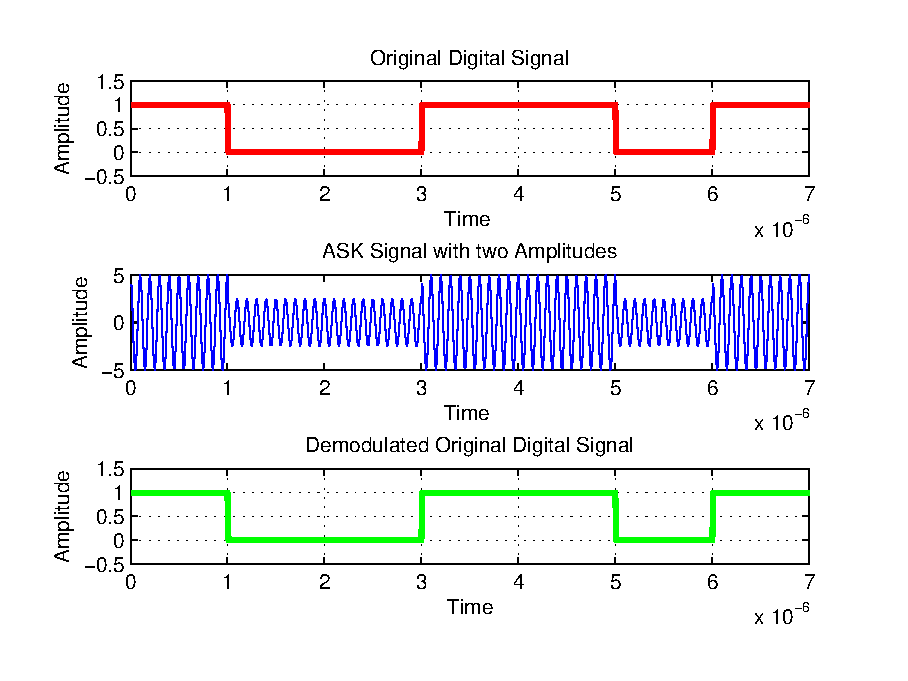
\includegraphics[width=0.7\textwidth]{ASKexample.eps}
    \caption[ASK modulation example]{ASK modulation example in the absence of noise for amplitudes $a_1=2.5$ and $a_2=5$.}
    \label{fig:ask}
\end{figure}

It is important to have an high signal-to-noise ratio (SNR), especially when the amplitudes are close so that the demodulator is able to identify them. The ASK scheme is very sensitive to atmospheric noise, distortions and propagation conditions.  A possible demodulator is shown in figure \ref{fig:askdem}.

\begin{figure}[h]
  \centering
    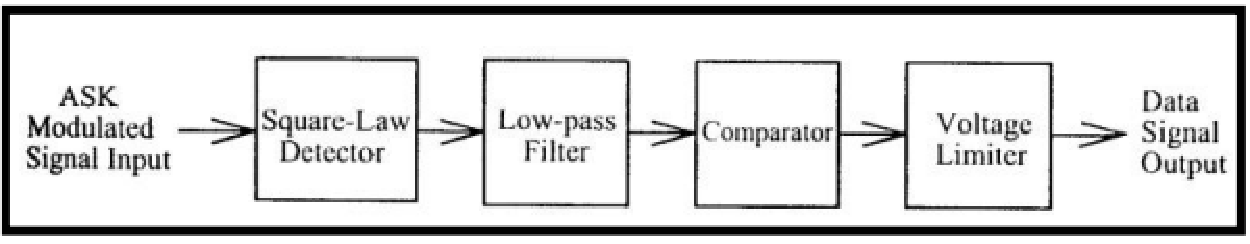
\includegraphics[width=0.7\textwidth]{askdem.pdf}
    \caption[Possible demodulator for ASK]{Possible demodulator for ASK\cite{ASKDemGaza}.}
    \label{fig:askdem}
\end{figure}


\subsection{PSK}

Phase-shift keying (PSK) is a digital modulation scheme that conveys data by changing, or modulating, the phase of a carrier wave. A finite number of phases are assigned to an unique pattern of binary digits. Usually, each phase encodes an even number of bits. The demodulator, which is designed specifically for the symbol-set used by the modulator, determines the phase of the received signal and maps it back to the corresponding signal. In digital phase modulation, the number of signal waveforms $M$ is represented as: 

\begin{equation}\label{Eq:PSK symbol}
\begin{array}{*{20}{c}}
{{s_i}(t) = }&{A\cos ({\omega _c}t + {\phi _i}(t)) = \overbrace {A\cos ({\phi _i}(t))}^{in - phase\;{\rm{symbol}}\;{{\rm{x}}_i}(t)} \cdot \cos ({\omega _c}t) \underbrace {-A\sin ({\phi _i}(t))}_{quadrature\;{\rm{symbol}}\;{{\rm{x}}_q}(t)} \cdot \sin ({\omega _c}t)}\\
{}&{ = {x_i}(t)\cos ({\omega _c}t) + {x_q}(t)\sin ({\omega _c}t)} \ ,
\end{array}
\end{equation}
where $A$ is the amplitude of the signal and ${\omega _c}$ is the carrier frequency in radians per second. The decision regions for two different M-PSK schemes are depicted in figure \ref{fig:pskdr}.

  
 Alternatively, instead of using the bit allocation to set the carrier's phase it can be used to change the phase by a given angle. Therefore, the demodulator determines the changes in the phase of the received signal, rather than the phase. Since this scheme depends on the difference between successive phases it is called differential phase-shift keying (D-PSK). 
 \begin{figure}[H]
  \centering
    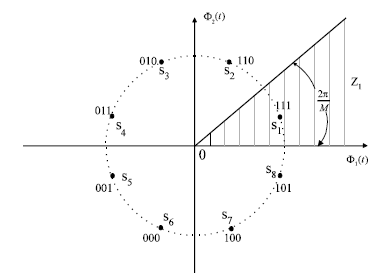
\includegraphics[width=0.4\textwidth]{PSKmodulation.png}
    \caption[Decision regions for 8-PSK]{Decision regions for 8-PSK. The minimum distance between symbols is given by $d_{min}=A\sin\frac{2\pi}{M}$  \cite{XiongDigModTech}.}
    \label{fig:pskdr}
\end{figure}


One of the advantages of PSK/D-PSK is that it is more bandwidth efficient compared to the FSK scheme. However, the signal detection/recovery is much harder compared to ASK and FSK since the demodulator must determine the phase of received sinusoid with respect to some reference phase. Additionally, if a higher rate PSK scheme is used, the equipment must be capable of distinguishing small differences in phase, making it unusable in time-varying channels.

\subsection{FSK}
\label{subsec:fsk}
Frequency shift keying (FSK) is a modulation technique in which data is transmitted through discrete frequency changes of a carrier wave with fixed amplitude $A$.  In figure \ref{fig:fskex} the simplest form of FSK (e.g. binary FSK or BFSK) is illustraded. A sinusoid carrier $s_i(t)$ is transmitted for each bit, zero or one, using the carrier frequencies $f_0$ and $f_1$, respectively. 

\begin{figure}[H]
  \centering
    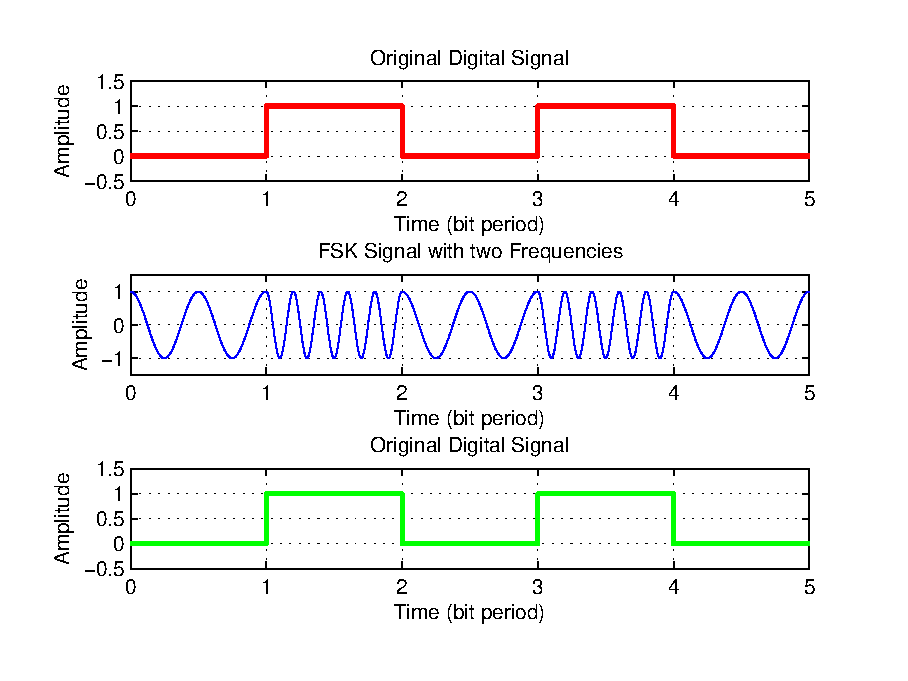
\includegraphics[width=0.7\textwidth]{fskexample.eps}
    \caption[BFSK example]{BFSK example for 2 low frequency carriers.}
    \label{fig:fskex}
\end{figure}

We can use multiple carriers to transmit $n>1$ bits. In order to guarantee that the symbols are orthogonal there should be a $\Delta f=\frac{k}{2T}$ separation among the  $M=2^n$ carrier frequencies, where $k$ is an integer and $T$ is the bit period. The complex baseband signalling waveforms for M-ary FSK \cite{Madhow} are given in the following equation:

\begin{equation}\label{Eq:M-FSK symbols}
{s_i}(t) = {e^{j2\pi {f_i}t}}{I_{[0,T]}},i = 1,2,...,M
\end{equation}



Coherent and non-coherent demodulation methods exist and depend on whether the phase of the sinusoids $\phi$ are equal or not. Coherent demodulators consist of correlators (matched filters) and samples, but they require synchronisation of the reference signals. The demodulator for BFSK can be implemented with two correlators as shown in figure \ref{fig:FSKdemcoherent}. This receiver is optimum in the sense that it minimizes the error probability for equally-likely binary signals. If for example a sinusoid carrier with frequency $f_1$ is transmitted, the upper correlator yields a signal $l_1$ with a positive signal component while $l_2$ has only a noise component. This is due to orthogonality of the signals.
  In case there is no phase reference, additional squarers or envelope detectors must be used for the non-coherent detection. In the last case, a minimum tone spacing of $\frac{k}{T}$ is required instead. The correlator implementation for non-coherent BFSK is illustrated in figure (\ref{fig:FSKdemNoncoherent}).

 \begin{figure}[H]
 \centering
\begin{subfigure}[h]{0.9\textwidth}
 \centering
    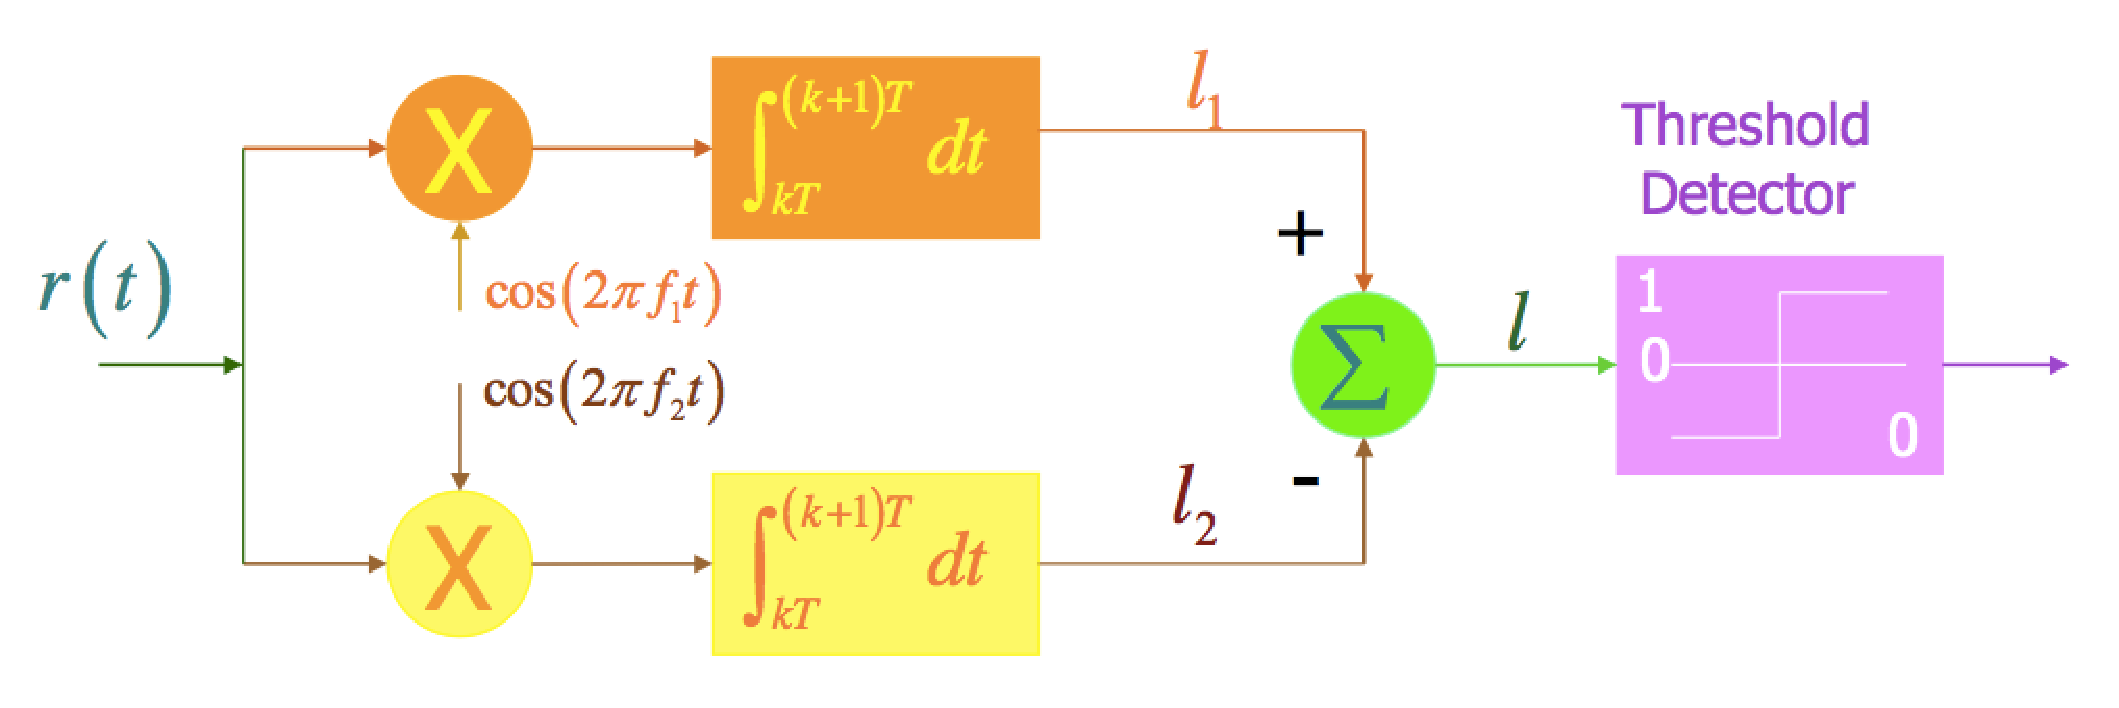
\includegraphics[width=0.6\textwidth]{fskdem1.pdf}
    \subcaption{Coherent.}
    \label{fig:FSKdemcoherent}

\end{subfigure}
\quad

\begin{subfigure}[H]{0.9\textwidth}
 \centering
    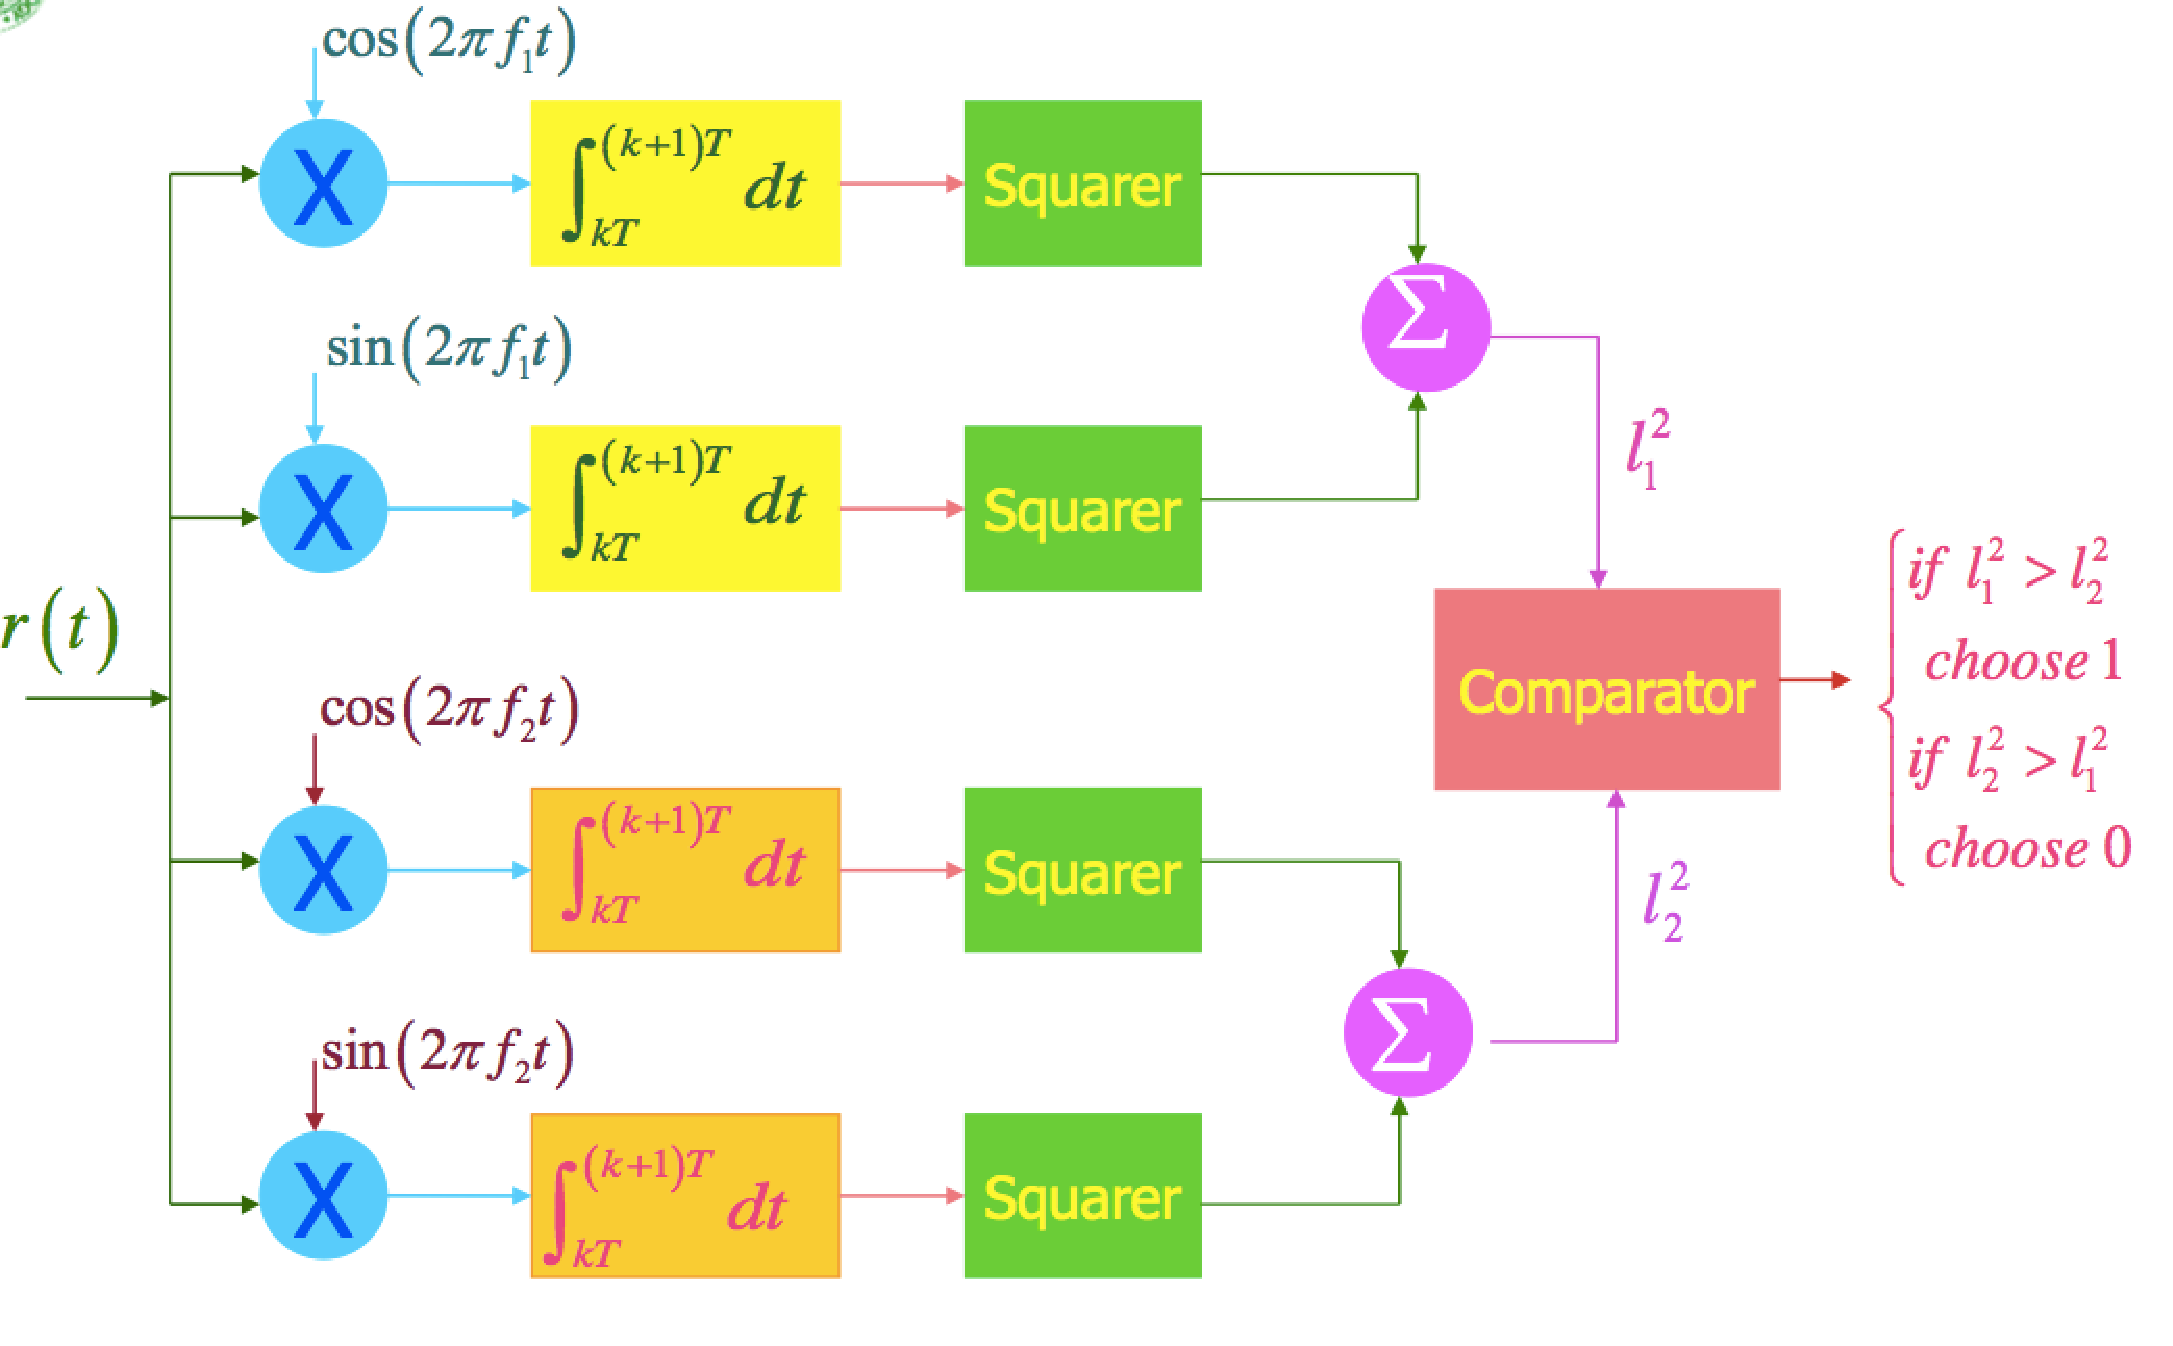
\includegraphics[width=0.6\textwidth]{fskdem2.pdf}
    \subcaption{Non-coherent.}
    \label{fig:FSKdemNoncoherent}
    \end{subfigure}
    \caption[Possible Demodulators for FSK]{Possible Demodulators for FSK \cite{DigModTech}.}
\end{figure}


It is expected that the error performance for the non-coherent receivers is greater than the coherent ones. However, the degradation is only a fraction of a decibel. Other options for demodulation are available such as the use of FFT schemes for peak picking or bandpass filtering at the working frequencies.

 \subsubsection{Performance}
 
 FSK systems have the highest power efficiencies among the available modulation schemes but they suffer from the low bandwidth (BW) efficiency. The main advantages of this modulating scheme are: the in-sensitiveness to amplitude variations in the channel, its compatibility with non-linear transmitters and receivers, and that it is not required to have an absolute frequency accuracy for correct demodulation (making it tolerant to local oscillators, drifts and Doppler shifts). One of the drawbacks is the fact that it is less bandwidth efficient when compared with other schemes such as ASK or PSK. To avoid undesirable spectral characteristics (which could cause adjacent channel interference) continuous phase FSK is required (see figure \ref{fig:comparecpfsk} for comparison).
%
 \begin{figure}[H]
 \centering
	\begin{subfigure}[H]{0.9\textwidth}
 \centering
    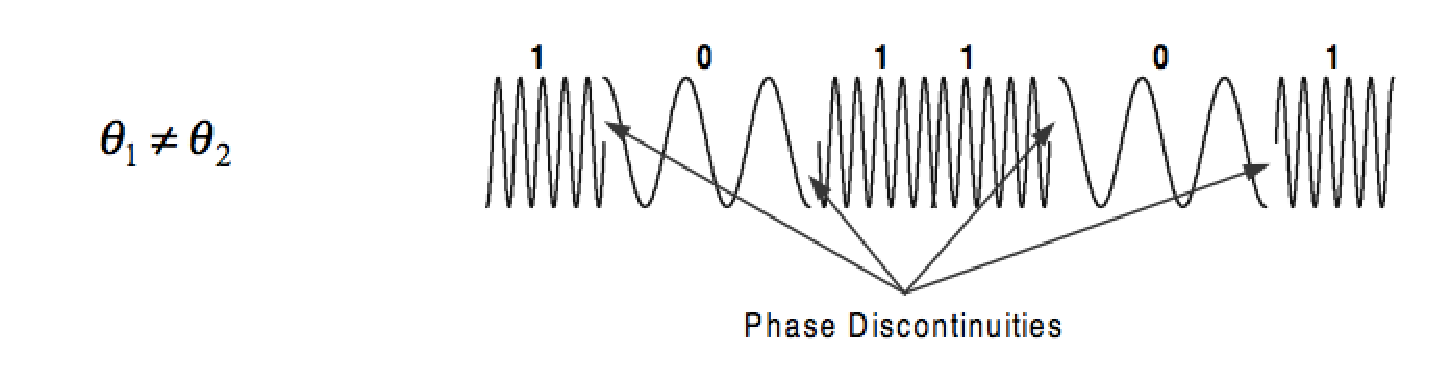
\includegraphics[width=0.6\textwidth]{ncpfsk.pdf}
    \subcaption{Non continuous phase FSK.}
    \label{fig:FSKcoherent}

	\end{subfigure}
	\quad

	\begin{subfigure}[H]{0.9\textwidth}
 	\centering
    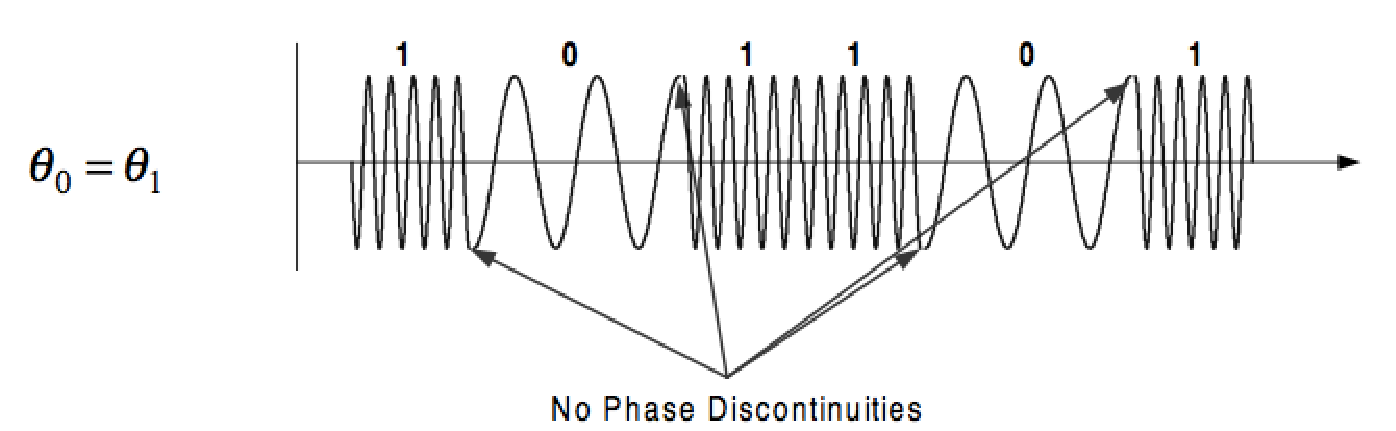
\includegraphics[width=0.6\textwidth]{cpfsk.pdf}
    \subcaption{Continuous phase FSK.}
    \label{fig:FSKnoncoherent}
 	\end{subfigure}
    \caption[FSK modulated signal]{FSK modulated signal, with and without phase discontinuity\protect\cite{DigCommLec}.}
    \label{fig:comparecpfsk}
\end{figure}

The M-ary FSK modulated signals can be written as follows:

\begin{equation}\label{Eq:M-FSK symbol 2}
{s_m}(t) = A{\varphi _m}(t),\quad 0 \le t \le T_s
\end{equation}

We can read $T_s$, from equation \ref{Eq:M-FSK symbol 2}, as the period of the input symbol stream, and $A$ as the amplitude of the basis function $\varphi_m$. In addition, the basis functions can be described by:

\begin{equation}\label{Eq:M-FSK basis}
{\varphi _m}(t) = \sqrt {\frac{2}{T}} \cos \left( {2\pi ({f_c} + {\alpha _m}\Delta {f_c}) + {\theta _m}} \right), \quad 0 \le t \le T
\end{equation}

where \[
{\alpha _m} \in \left\{ {(2m - 1 - M) | m = 1,2,...,M} \right\}
\] 
In order to satisfy orthogonality the inner product between the basis functions must be 1 for $m=n$ and 0 for $m\neq n$:
\begin{equation}\label{Eq:M-FSK inner product}
\left\langle {\left. {{\varphi _m},{\varphi _n}} \right\rangle } \right. = \int {{\varphi _m}(t){\varphi _n}(t)dt = {\delta _{mn}} = \left\{ \begin{array}{l}
1,m = n\\
0,m \ne n
\end{array} \right.}
\end{equation} 


Individual frequencies corresponding to different symbols are given by equation \ref{Eq:M-FSK fm},
\begin{equation}\label{Eq:M-FSK fm}
{f_m} = {f_c} + {\alpha _m}\Delta {f_c}
\end{equation}
where $f_c$ is the central frequency and $\Delta f_c$ is the frequency separation.\\

In order to satisfy orthogonality \cite{gold} must apply:

\begin{equation}\label{Eq:M-FSK deltaF}
\Delta {f}= 2\Delta {f_c} = \left\{ \begin{array}{l}
\frac{1}{{2T}}, \quad {\theta _m} = {\theta _n}, \quad \forall m,n\\
\frac{1}{T}, \quad {\theta _m} \ne {\theta _n}
\end{array} \right.
\end{equation}

The overall bandwidth occupied by the FSK signal depends on the modulation index $h$ described in equation \ref{Eq:M-FSK mod index}.
\begin{equation}\label{Eq:M-FSK mod index}
h=\frac{2\Delta {f_c}}{R}=2\Delta {f_c}T_s 
\end{equation}

For continuous phase BFSK the minimum value for the signals to not interfere with each other is $h=0.5$. An FSK system using continuous phase transitions has much lower side-lobe energy than the discontinuous case. All these parameters will cause inter-symbol-interference (ISI) and limit the rate of the system. For this reason it is important to further increase the bandwidth efficiency of the system by applying pulse shaping to the transmitted signal. This technique is described in section \ref{Sec:Pulse shapping}. 



\subsection{M-QAM}
M-ary Quadrature-Amplitude modulation is a two-dimensional signalling scheme that combines both Amplitude and Phase Shift Keying. The transmitted signal for every symbol can be written as \cite{Proakis}:
\begin{equation}\label{Eq: MQAM symbols}
{s_i}\left( t \right) = \sqrt {\frac{{2{E_0}}}{T}} {a_i}\cos \left( {2\pi {f_c}t} \right) - \sqrt {\frac{{2{E_0}}}{T}} {b_i}\sin\left( {2\pi {f_c}t} \right), \quad \left\{ {\begin{array}{*{20}{c}}
{0 \le t \le T}\\
{i = 0, \pm 1, \pm 2, \ldots }
\end{array}} \right.
\end{equation}

The typical in phase (I) and quadrature (Q) known as IQ modulation and demodulation is shown in figure \ref{fig:iqmodem}. We consider that the information to be transmitted is a complex signal $x=x_i+jx_q$. Ignoring the energy and period factors, the output of the IQ modulation transmitter is given by \cite{Madhow}:

\begin{equation}\label{EQ: MQAM IQ}
y(t) = \Re \{ x{e^{j2\pi {f_c}t}}\}  = {x_i}\cos (2\pi {f_c}t) - {x_q}\sin (2\pi {f_c}t)
\end{equation}

 \begin{figure}[H]
  \centering
    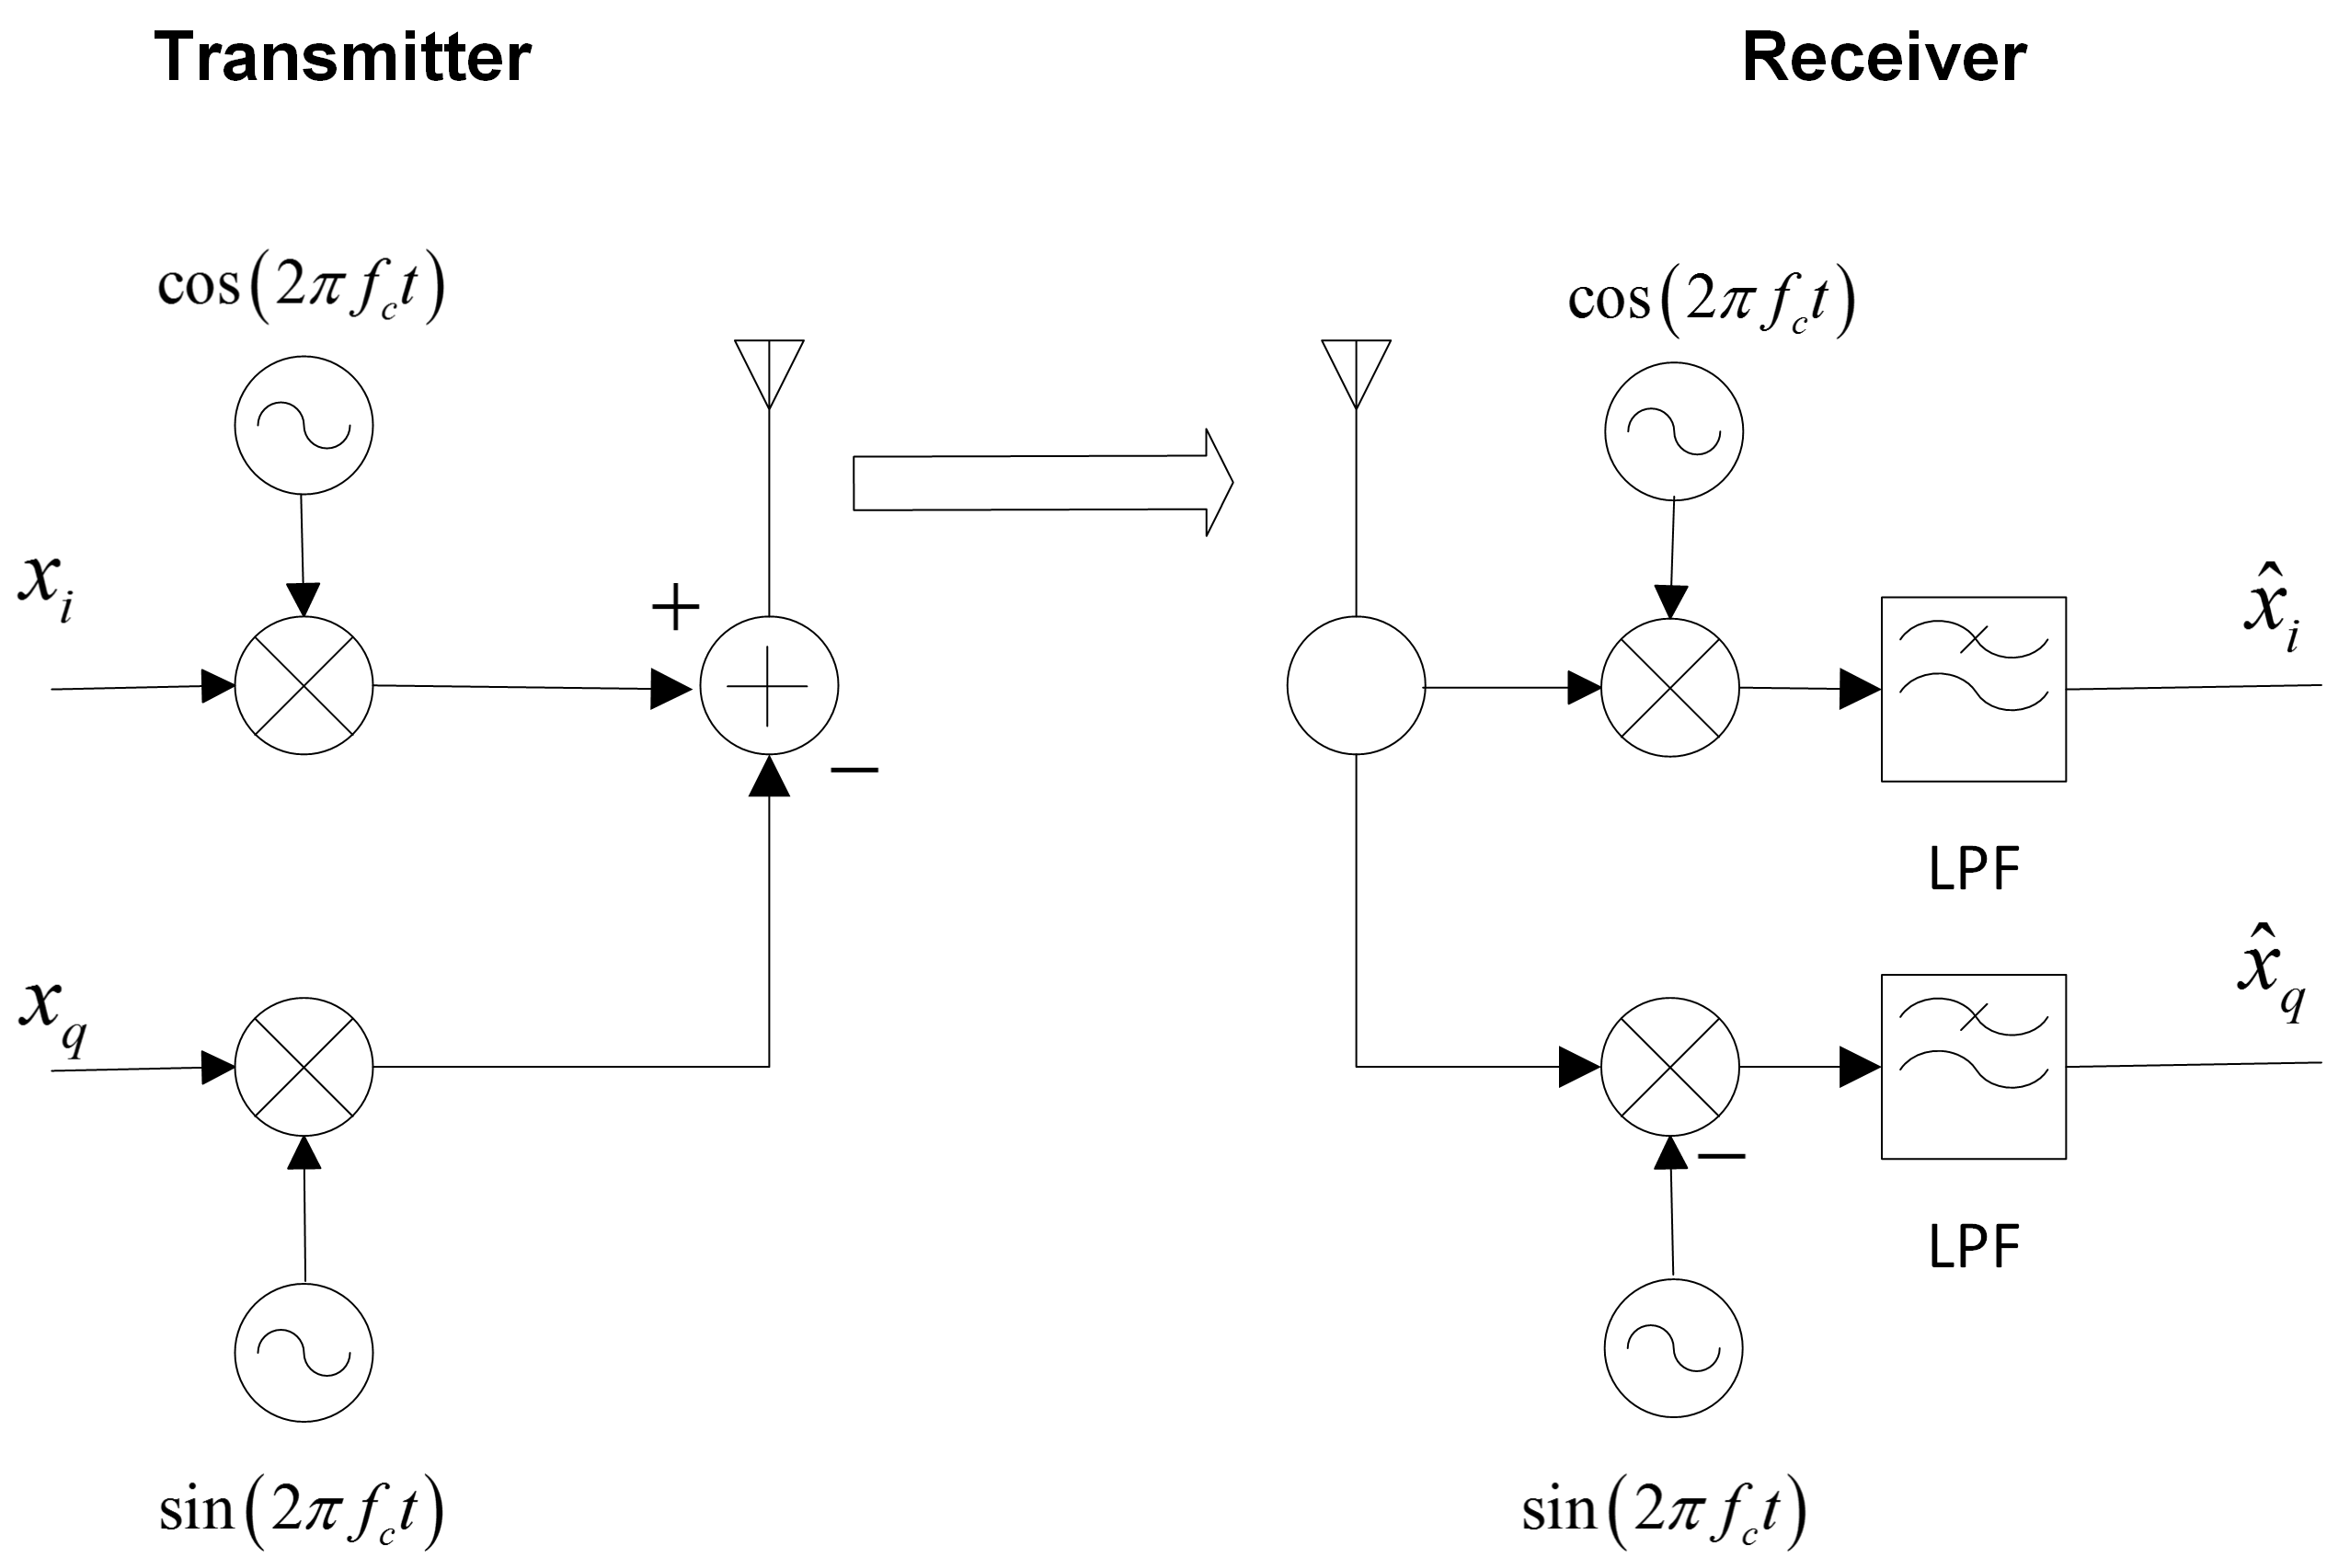
\includegraphics[width=0.7\textwidth]{MQAMsyst.png}
    \caption[Schematic of M-QAM transmitter and receiver]{Schematic of M-QAM transmitter and receiver showing the in-phase (I) and quadrature (Q) components.}
    \label{fig:iqmodem}
\end{figure}



At the transmitter the information $x_i$ is mapped to $\cos (2\pi {f_c}t)$ and $x_q$ is mapped to $\sin (2\pi {f_c}t)$. At the receiver we multiply the signal with $\cos (2\pi {f_c}t)$ and $-$$\sin (2\pi {f_c}t)$ followed by low-pass filtering to extract $\hat{x}_i$ and $\hat{x}_q$. The mathematical expressions for the recovered information at the receiver, using the trigonometric identities, can be summarized as followed \cite{Madhow}: 

\begin{eqnarray}
{{\hat x}_i} = \int\limits_0^T {y \cdot \cos (2\pi {f_c}t)dt = } \int\limits_0^T {\left( {{x_i}\cos (2\pi {f_c}t) - {x_q}\sin (2\pi {f_c}t)} \right) \cdot \cos (2\pi {f_c}t)dt\mathop  = \limits^{LPF} \frac{{{x_i}}}{2}}\\
{{\hat x}_q} = \int\limits_0^T { - y\cdot \sin (2\pi {f_c}t)dt = } \int\limits_0^T { - \left( {{x_i}\cos (2\pi {f_c}t) - {x_q}\sin (2\pi {f_c}t)} \right) \cdot \sin (2\pi {f_c}t)dt\mathop  = \limits^{LPF} \frac{{{x_q}}}{2}} 
\end{eqnarray}

By ignoring the scaling factor of $\frac{1}{2}$ and assuming that the channel is ideal, both $x_i$ and $x_q$ can be recovered successfully. 

\subsubsection{QAM symbol mapping}

As stated previously the QAM scheme involves sending digital information by periodically adjusting the phase and amplitudes of a sinusoidal wave. For example 4-QAM consists of four unique combinations of phase and amplitude. These combinations, called symbols, are shown as the white dots on the constellation plot in figure \ref{fig:4qamsym}. It is possible to send up to two bits per symbol when using 4-QAM modulation. It is also possible to send data at even higher rates by increasing the number of symbols in our symbol map. By convention the number of symbols in a symbol map is called the symbol map “M” and is considered the “M-ary” of the modulation scheme. The number of bits in an M-QAM scheme is given by ${{{\log }_2}M}$. 


 \begin{figure}[H]
  \centering
    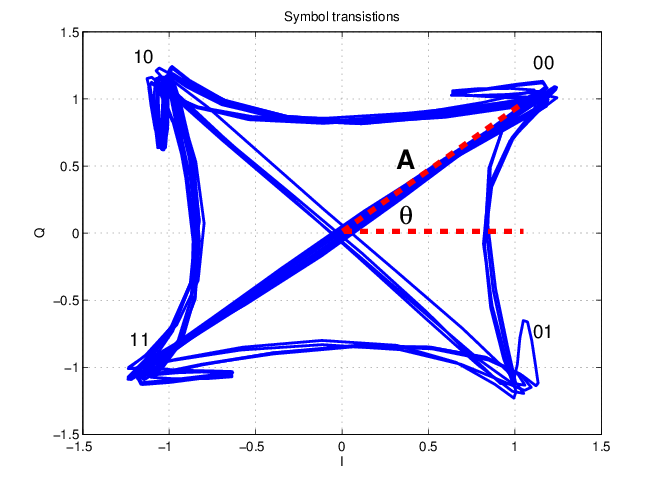
\includegraphics[width=0.7\textwidth]{4symboltransitions.png}
    \caption[Constellation plot of combinations of phase and amplitude in 4-QAM]{Constellation plot of combinations of phase and amplitude in 4-QAM. The blue lines represent the phase and amplitude transitions from one symbol to another. Labelled in the constellation plot, there is the digital bit pattern that each symbol represents.}
    \label{fig:4qamsym}
\end{figure}



\subsubsection{Impairments}
Although QAM appears to increase the transmission efficiency for digital communication systems by utilising both amplitude and phase variations, it has a number of drawbacks. It is more susceptible to noise because the states are closer together. This means a lower level of noise is needed to move the signal to a different decision point. The second limitation is that linearity must be maintained when the signal is passed through the channel and amplifiers. Both these limitations are associated with the amplitude component of the signal. 

In an ideal I-Q modulator the phase difference between the signals used for modulating the I and Q arm is 90 degrees, resulting in using $\cos (2\pi {f_c}t)$ and $\sin (2\pi {f_c}t)$ for sending $x_i$ and $x_q$. If there is phase imbalance, the phase difference might not be exactly 90 degrees. In that case, we can consider that $\cos (2\pi {f_c}t)$ and $\sin (2\pi {f_c}t + \varphi )$ carriers are used for transmitting instead.
When there is amplitude imbalance there will be added small level variations in the sine and cosine carriers at the modulator. This can be modelled by using $\cos (2\pi {f_c}t)$ for the in-phase component $x_i$ and  $(1 + \alpha )\sin (2\pi {f_c}t)$ to carry the quadrature component $x_q$.

The transmitted signal including the effect of phase and amplitude imbalance is then \cite{Madhow}:
\begin{equation}\label{MQAM impaired rcvd signal}
y(t) = {x_i}\cos (2\pi {f_c}t) - {x_q}(1 + \alpha )\sin (2\pi {f_c}t + \varphi ) \text{,\quad where 0} < \text{$\alpha$} < \text{1}
\end{equation}

Assuming that we have an ideal IQ demodulator at the receiver we split and multiply the signal $y(t)$ with $\cos (2\pi {f_c}t)$  and $\sin (2\pi {f_c}t)$ carriers. The outcome of such multiplications is low-pass filtered, allowing to extract  $\hat{x}_i$ and $\hat{x}_q$, respectively:
\begin{eqnarray}
{{\hat x}_i} & = & \frac{1}{2}\left[ {{x_i} - {x_q}(1 + \alpha )\sin (\varphi )} \right]\\
{{\hat x}_q} & = & \frac{1}{2}\left[ {{x_q}(1 + \alpha )\cos (\varphi )} \right]
\end{eqnarray}

These non-idealities leads to a quadrature skew that causes a different mapping in both the transmitter and receiver. IQ gain imbalance equates to a rectangular stretch along the IQ axis. Likewise, quadrature error results in the IQ axis not being exactly $90\degree$ apart. These phenomena can be seen in figure \ref{fig:skewed}.


\begin{figure}[H]
 \centering
	\begin{subfigure}[H]{0.9\textwidth}
 	\centering
    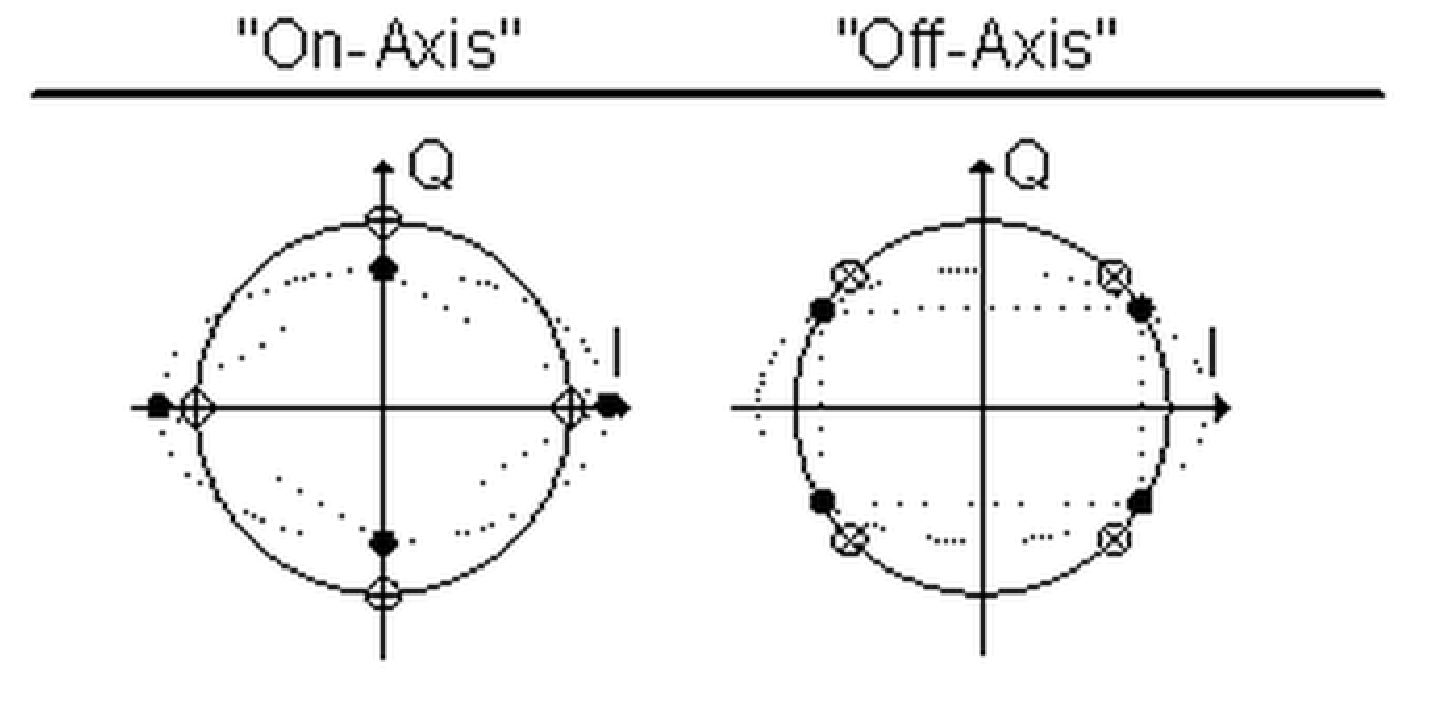
\includegraphics[width=0.6\textwidth]{gi.pdf}
    \subcaption{IQ gain imbalance.}
    %%\label{}

	\end{subfigure}
	
	\begin{subfigure}[H]{0.9\textwidth}
 	\centering
    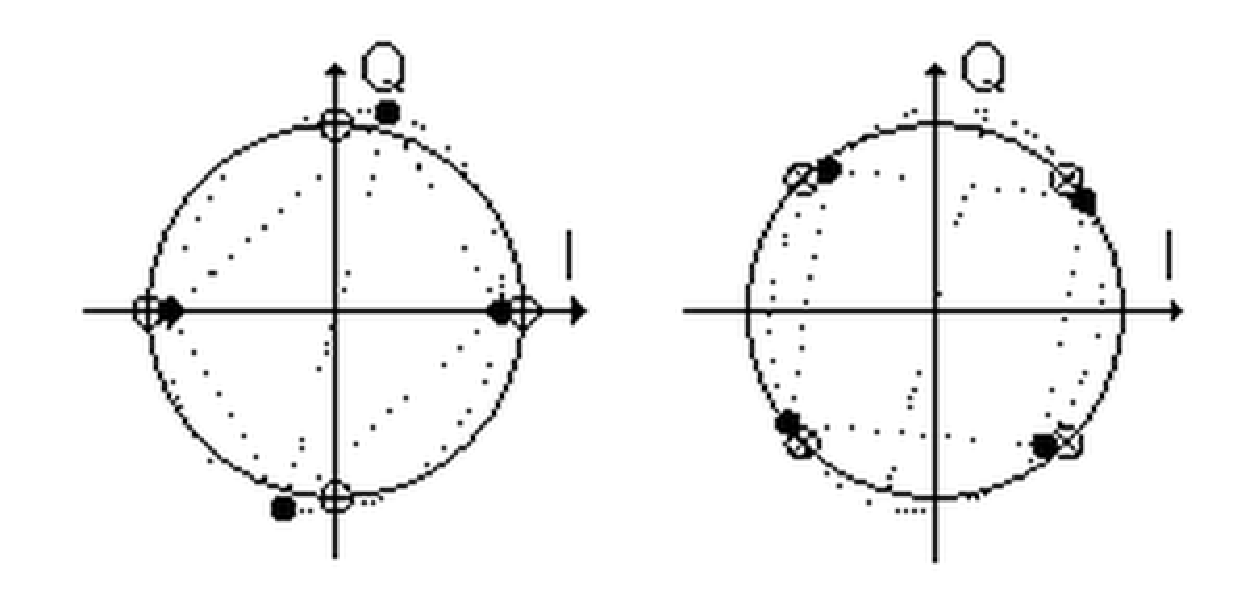
\includegraphics[width=0.5\textwidth]{qe.pdf}
    \subcaption{IQ quadrature error.}
   %% \label{}
 	\end{subfigure}
    \caption[Two possible constellation mapping for 4-QAM]{Two possible constellation mappings for 4-QAM and the effects of impairments on phase and amplitude\cite{Agilent IQ paper}.}
    \label{fig:skewed}
\end{figure}


\subsubsection{Performance and Impact of Noise}
\label{sec:MQAMperf}
When studying the impact of the noise in QAM systems we assume that Gray coding is used, all symbols are equiprobable, the noise is zero-mean additive white gaussian noise (AWGN) with variance $\frac{N_0}{2}$ and there are no errors from carrier recovery or symbol synchronisation. In a square M-QAM system the amplitudes of $x_i$ and $x_q$ can take $\log_2{M}$ different values. Each level can be \
$ -(\sqrt M  -1)d, - (\sqrt M  - 3)d,\cdots,(\sqrt M  - 1)d $, where $d$ is half of the minimum distance between two symbols. The value of $d$ can be computed as \cite{BER-QAM paper}: 
\begin{equation}\label{Eq: MQAM min dist}
d = \sqrt {\frac{{3{{\log }_2}(M) \cdot {E_b}}}{{2(M - 1)}}}\ ,
\end{equation}
where $E_b$ is the energy per bit in the transmitter. Recall that at the demodulator, the received vector is given by \cite{BER-QAM paper}: 
\begin{equation}
 \mathbf{r}=\mathbf{s}+\mathbf{n}=\left[ \begin{array}{l}I\\Q \end{array} \right] + \left[ \begin{array}{l}{n_i}\\{n_q}\end{array} \right]\ ,
\end{equation}


The proof of the BER expression for the MQAM is out of the scope of this report. However the final generic result is given as: 
\begin{equation}\label{Eq: BER MQAM}
{P_b} = \frac{1}{{{{\log }_2}\sqrt M }}\sum\limits_{k = 1}^{{{\log }_2}\sqrt M } {{P_b}(k)}\ ,
\end{equation}


The conditional BER,  $P_b(k)$ in equation \ref{Eq: BER MQAM}, corresponding to the k-th bits $(k=1,2,3,... \log_2{\sqrt{M}} )$ on both I and Q components is defined as follows \cite{BER-QAM paper}:
\begin{equation} \label{eq:mqamBER}
{P_b}(k) = \frac{1}{{\sqrt M }}\sum\limits_{j = 0}^{(1 - {2^{ - k}})\sqrt M  - 1} {\left[ {{{( - 1)}^{\left\lfloor {\frac{{j{2^{k - 1}}}}{{\sqrt M }}} \right\rfloor }}\left( {{2^{k - 1}} - \left\lfloor {\frac{{j{2^{k - 1}}}}{{\sqrt M }} + \frac{1}{2}} \right\rfloor } \right) \cdot \text{erfc}\left( {(2j + 1)\sqrt {\frac{{3{{\log }_2}(M) \cdot {E_b}}}{{2(M - 1){N_0}}}} } \right)} \right]}
\end{equation}

The outcome of these expressions is displayed in figure \ref{fig:mqamber}.

 \begin{figure}[H]
  \centering
    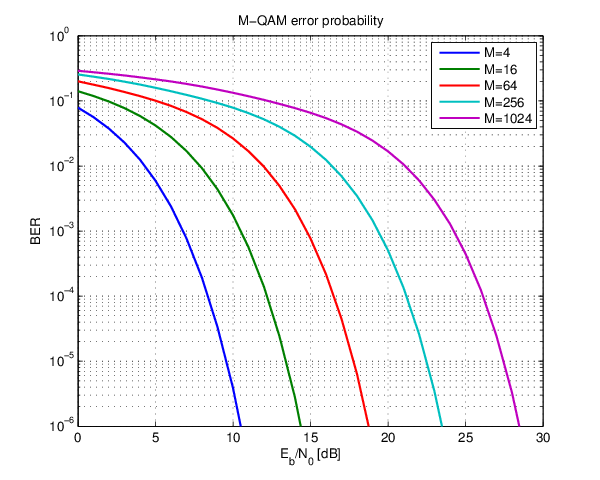
\includegraphics[width=0.5\textwidth]{MQAMber.png}
    \caption[BER performances of M-ary QAM]{BER performances of M-ary QAM.}
    \label{fig:mqamber}
\end{figure}




\subsection{OFDM}

OFDM or Orthogonal Frequency-Division Multiplexing is a multi-carrier modulation scheme that divides the available bandwidth $W$ into $N$ sub-bands with relatively narrow width, $\Delta f = \frac{W}{N}$. The signal in each sub-band can be independently encoded and modulated as a synchronous symbol with rate $T = \frac{1}{\Delta f}$. If $\Delta f$ is small enough the channel frequency response $C(f)$ is essentially constant across each sub-band. Hence, the ISI is negligible and OFDM provides a solution that could yield transmission rates close to the channel capacity. 

By choosing the modulating waveforms to be \emph{eigen-functions} of a linear-time invariant channel (LTI), it can be guaranteed that the waveforms will remain orthogonal after going through the channel. Therefore, the fact that complex exponentials $\exp{(j2\pi f_k t)}$ are orthogonal at different frequencies $f_k$  can be exploited.  Suppose that the $N$ data to be transmitted are $X_k, k=0,1,...,N-1$, where $X_k$ is a complex number in a given constellation. If a carrier frequency $f_k$ is assigned to each symbol $X_k$ and each contribution is summed at the output, the following result is obtained:

\begin{equation}
x(t) = \sum\limits_{k = 0}^{N - 1} {{X_k}{e^{j2\pi {f_k}t}}}
\end{equation}


For the implementation of a digital system a transmitter will generate its output in a sampled-data fashion. By letting $t=nT_s$ and $f_k=k\Delta f$, where $T_s$ is the sample interval and $\Delta f$ the sub-carrier spacing (assumed to be uniform), the output is given by:
\begin{equation}
x(n{T_s}) = \sum\limits_{k = 0}^{N - 1} {{X_k}{e^{j2\pi k\Delta fn{T_s}}}}
\end{equation}

The sub-carrier spacing should be computed such that the orthogonality of different sub-carriers holds over an interval of length $T$:

\begin{equation}
\int\limits_0^T {{e^{j2\pi {f_m}t}}{e^{ - j2\pi {f_n}t}}} dt = \frac{{{e^{j2\pi ({f_n} - {f_m})t}} - 1}}{{j2\pi ({f_n} - {f_m})}} = 0,{\text{ for }}({f_n} - {f_m})T  \in \mathbb{Z}_{\neq 0}
\end{equation}

Hence, $\Delta f = \frac{1}{NT_s}=\frac{1}{T}$ is the minimum separation to keep orthogonality among signals at different modulators, resulting in:
\begin{equation}
x(n{T_s}) = \sum\limits_{k = 0}^{N - 1} {{X_k}{e^{j2\pi kn/N}}} \text{, }n = 0,1,...,N - 1
\end{equation}


The above formula is the equation of an N-point IDFT for one OFDM symbol. If $N$ is a power of two the samples $x(nT_s)$ can be efficiently generated (for example by using the FFT algorithm). A plot of the resulting signal in time and frequency domain is shown in figure \ref{fig:ofdmsig}.

\begin{figure}[H]
 \centering
	\begin{subfigure}[H]{0.9\textwidth}
 	\centering
    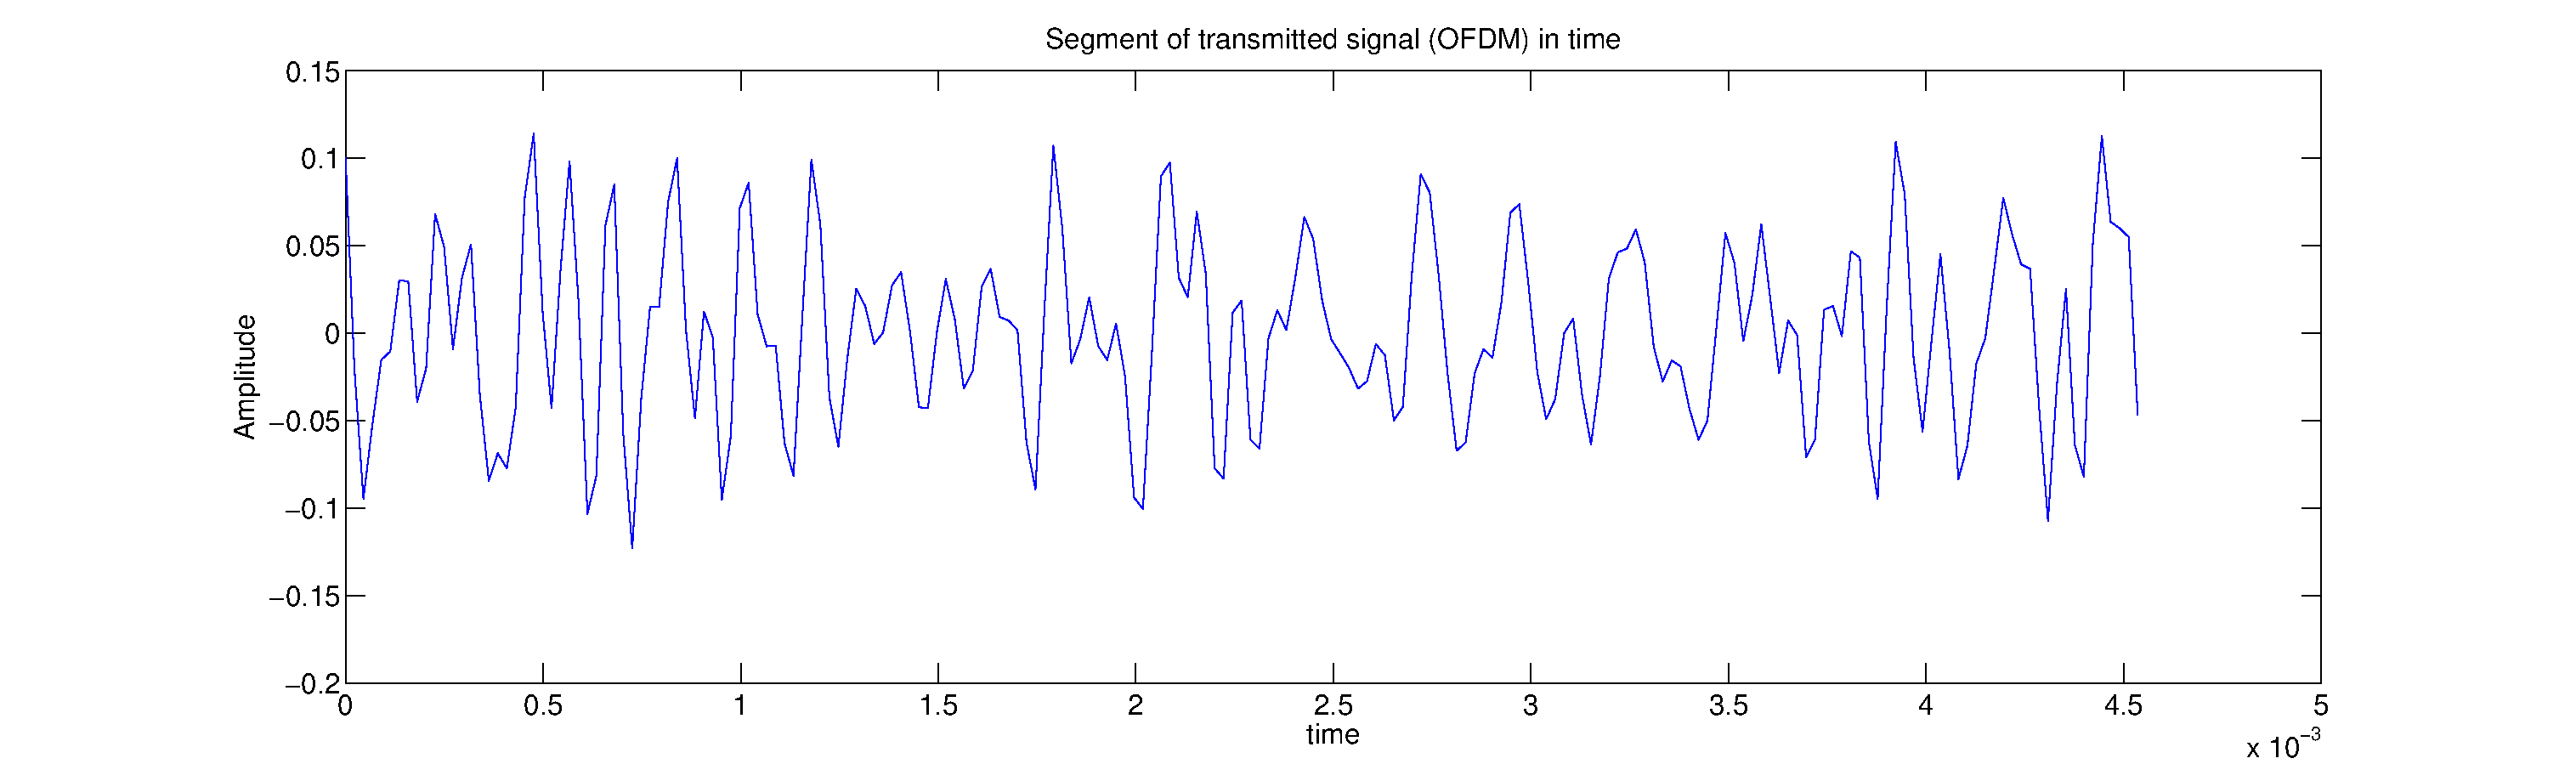
\includegraphics[width=0.9\textwidth]{ofdmsignal.eps}
    \subcaption{OFDM signal segment.}
    %%\label{}

	\end{subfigure}
	
	\begin{subfigure}[H]{0.9\textwidth}
 	\centering
    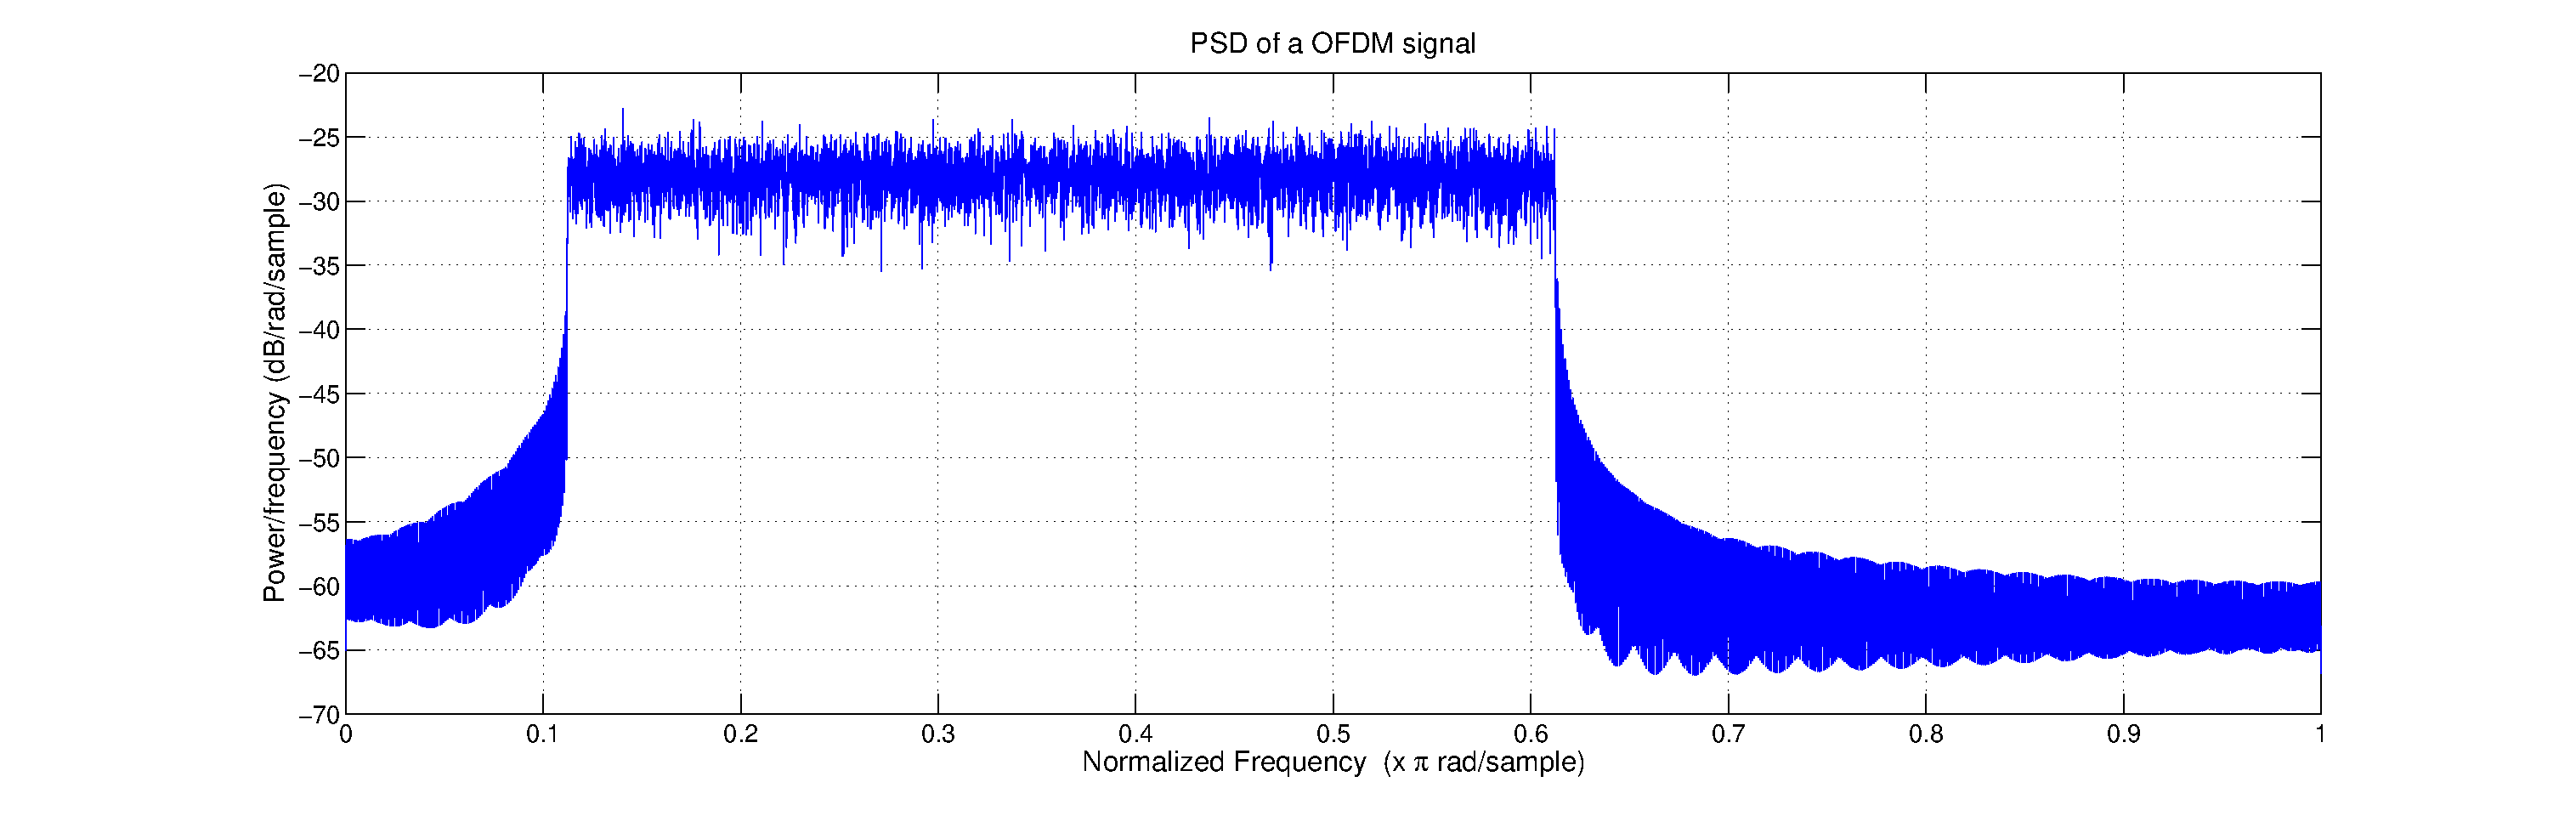
\includegraphics[width=0.9\textwidth]{psdofdm.eps}
    \subcaption{PSD of a OFDM signal}
   %% \label{}
 	\end{subfigure}
    \caption[OFDM signal segment and the PSD of a OFDM signal]{Example of an OFDM signal centred at 8 kHz with a DFT size of $N=2048$, the number of active subcarriers $N_c =512$ are with a sampling frequency of $f_s=44.1$ kHz.}
    \label{fig:ofdmsig}
\end{figure}


% %\subsubsection{OFDM impairments}
%\subsubsection{OFDM impairments - guard interval and guard band}
\textcolor{red}{Consider move this section after OFDM transceiver architecture}
In multi-path channels a receiver can receive several delayed replicas of the transmitted signal causing ISI. To eliminate the effect of inter symbol interference (ISI), a guard interval of $N_g$ samples is usually inserted at the beginning of each OFDM symbol. During the guard interval the transmitter can either:

\begin{itemize}
\item Zero pad (ZP) the transmission by sending a null waveform.

\item Introduce a cyclic prefix (CP) which is an exact copy of a segment of the OFDM symbol located towards the symbol end. A cyclic suffix can be used in a similar fashion.

\end{itemize}
Since ZP introduces inter-carrier interference(ICI) cyclic prefixing transmission is preferred. 
To prevent significant leakage to adjacent bands, OFDM systems usually do not transmit any data on the sub-carriers near the two edges of the allocated band. These unused sub-carriers are known as guard sub-carriers or virtual sub-carriers. The collection of all the unused sub-carriers is called the guard band. As the PSD of the OFDM signal has quite high sidelobes, to reserve a guard band helps to minimise out-of-band emissions and thus eases the requirements on transmitter front-end filters. Nevertheless, adoption of a guard band misspend assigned bandwidth and decreases the spectral efficiency of the OFDM system. In addition to guard bands some sub-carriers around DC frequency (subcarrier index 0) should be nullified in order to evade unwanted DC and low-frequency components generated by the receiver's front-end. Other issues may arise when using of OFDM such as spectral shaping and peak-to-average power ratio. These issues are discussed in section \ref{Sec:Pulse shapping}. 


\subsubsection{OFDM transceiver architecture}

A general OFDM transmitter integrates several functions including DFT processing, guard interval insertion and spectral shaping. In a receiver, besides DFT processing and guard interval removal, additional efforts are required to handle the channel-fading effect and synchronisation issues between the transmitter and receiver (discussed in section \ref{sec:ts}).
As it will be discussed in part \ref{sec:ts} the amplitude and phase maybe estimated via the use of a known training sequence. In an OFDM system these parameters should be estimated for each of the carriers frequencies. In the case of a time variant channel the new estimations can be done by inserting known reference symbols, sometimes referred to as pilot symbols, at regular intervals within the OFDM time-frequency grid. The effects of an amplitude varying channel and the previously mentioned grid are depicted in figure \ref{fig:ofdmchannel}.
\textcolor{red}{Add references and footnotes from books if they fit better.}
\begin{figure}[H]
 \centering
	\begin{subfigure}[H]{0.9\textwidth}
 	\centering
    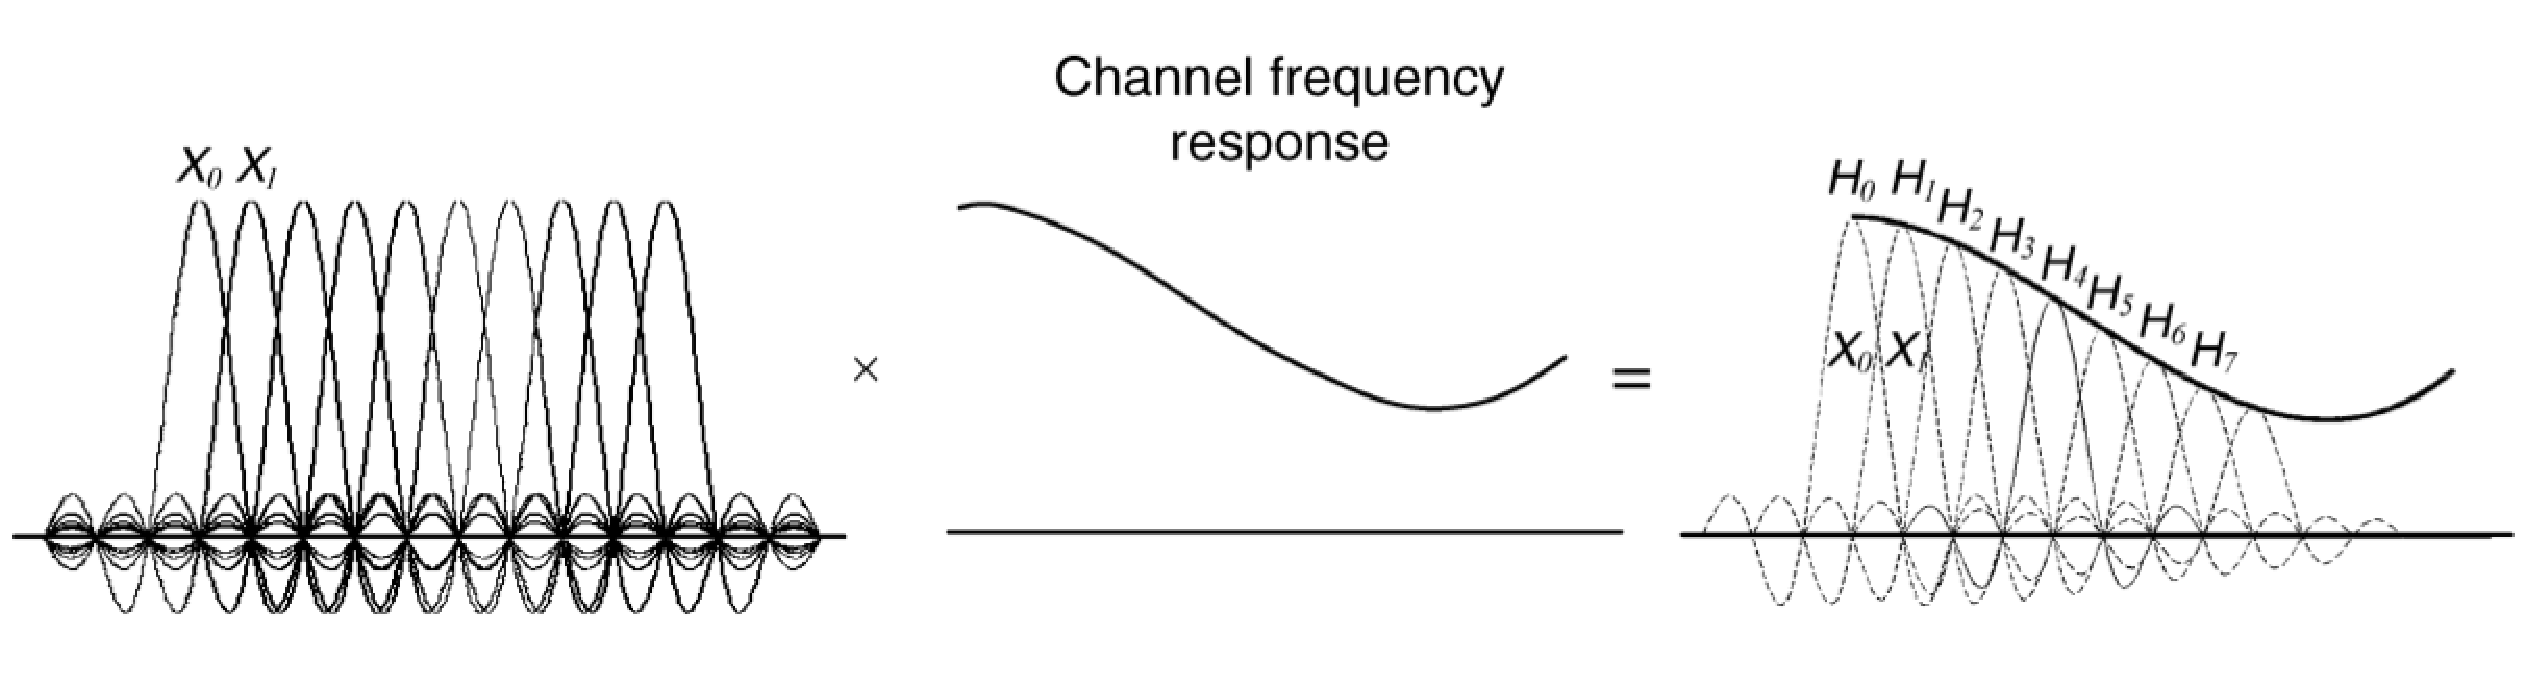
\includegraphics[width=0.9\textwidth]{ofdmchannel.pdf}
    \subcaption{The effects of a channel with non-flat frequency response to each subcarrier.}
    %%\label{}

	\end{subfigure}
	
	\begin{subfigure}[H]{0.9\textwidth}
 	\centering
    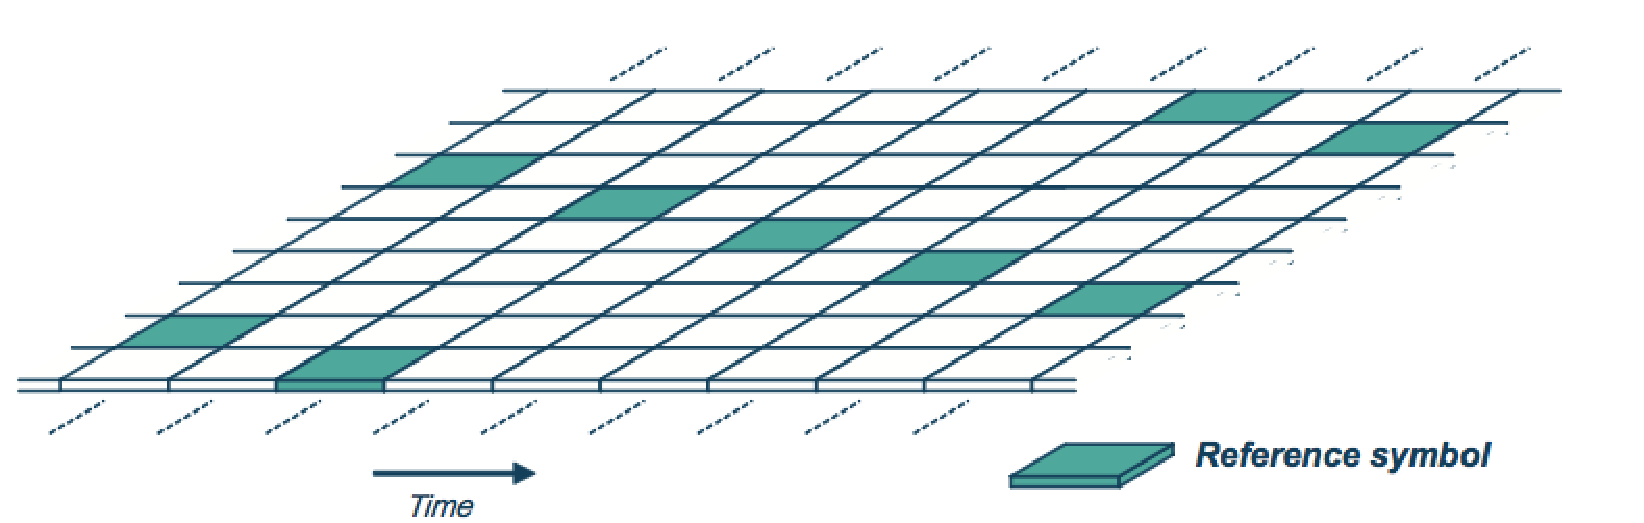
\includegraphics[width=0.7\textwidth]{ofdmgrid.pdf}
    \subcaption{Frequency-time grid containing the pilots. Reference symbols density should be chosen accordingly to the channel properties.}
   %% \label{}
 	\end{subfigure}
    \caption[The effects of a non-flat channel and a grid containing the OFDM pilot symbols]{The effects of a non-flat channel and a grid containing the OFDM pilot symbols, in time and frequency domains for channel estimation.}
    \label{fig:ofdmchannel}
\end{figure}

In the implementation of an OFDM communication system, the following basic OFDM parameters need to be decided upon:
\begin{itemize}
\item The subcarrier spacing $\Delta f = \frac{1}{T_u}$. The OFDM subcarrier spacing should be as small as possible to minimise the relative cyclic-prefix overhead $\frac{T_{CP}+T_{CS}}{T_u + T_{CP} + T_{CS}}$. However, a too small sub-carrier spacing increases the sensitivity of the OFDM transmission to Doppler spread and different kinds of frequency inaccuracies.

\item The total number of subcarriers, defined by the size of the DFT, and the number of active subcarriers $N_c$. This parameter will define the basic bandwidth occupied by the signal: 
\begin{equation}\label{eq:OFDMbw}
W = N_c \times \Delta f = \frac{N_c}{T_u}=\frac{N_c}{N_{FFT}}\times f_s
\end{equation}

\item The cyclic prefix and suffix length $T_g = T_{CP} + T_{CS}$, which will determine the overall symbol time $T = T_u + T_g$. In principle, the cyclic-prefix length $T_{CP}$, should cover the maximum length of the time dispersion that is expected in the channel. 
\end{itemize}

This parameters, along with others, will determine the performance of the system and, hence, must be chosen carefully. 

On the receiver side the, after the synchronization is complete, the inverse operations are perfomed, like depicted in figure \ref{fig:ofdmtransceiver}

 \begin{figure}[H]
  \centering
    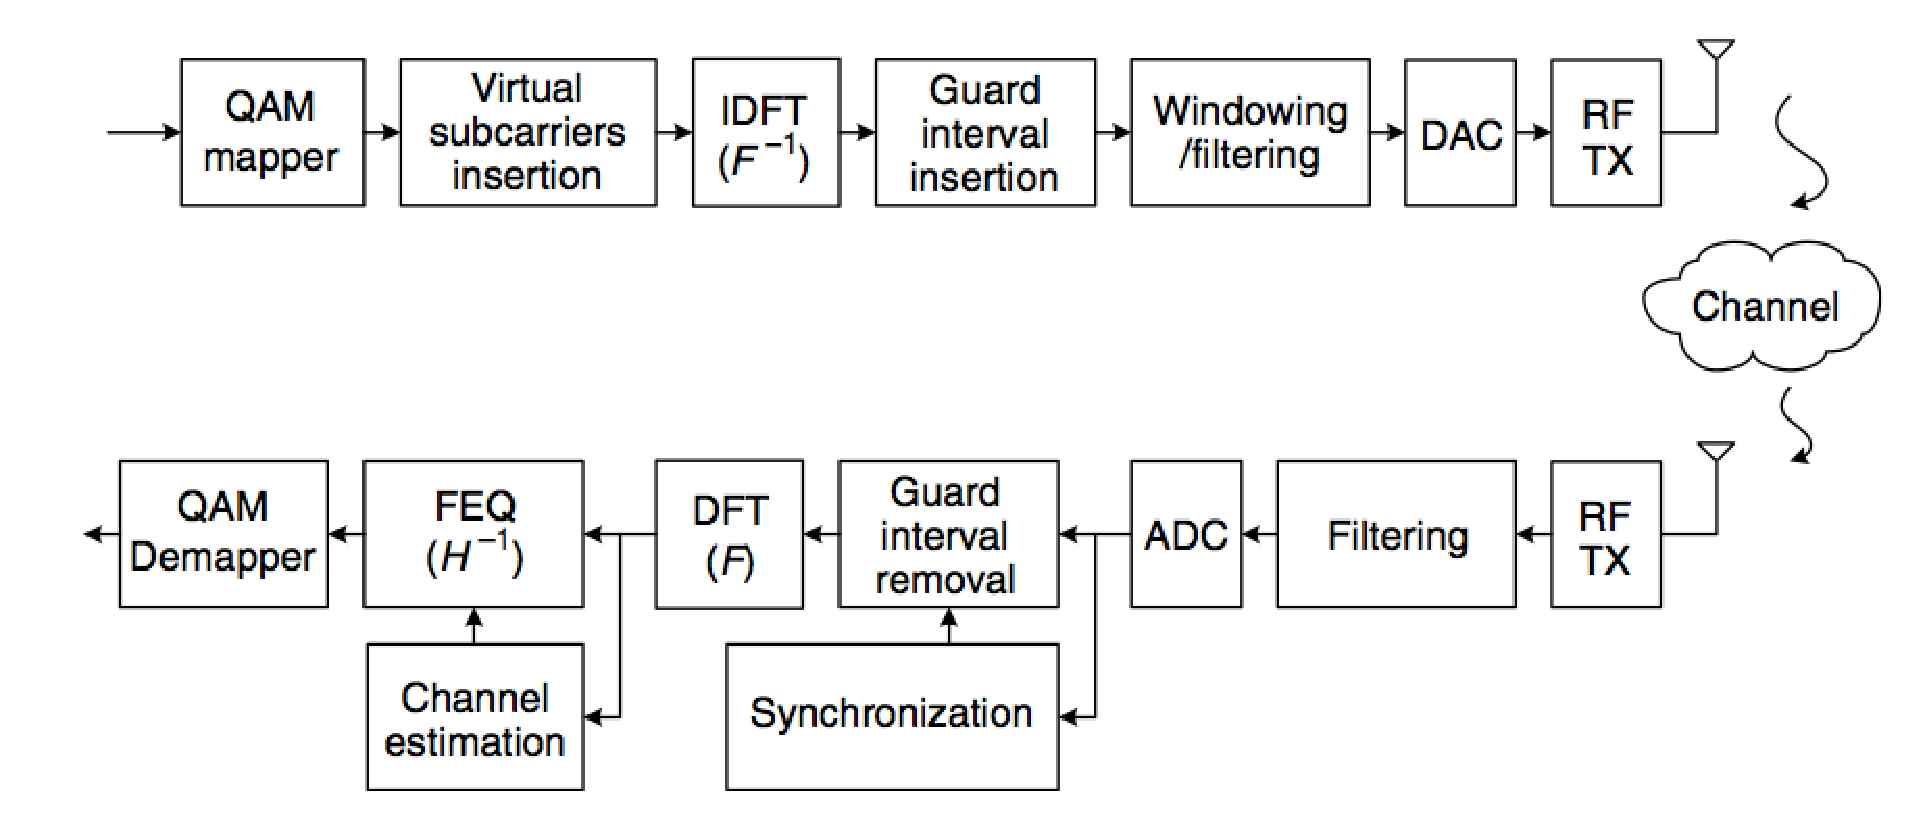
\includegraphics[width=0.8\textwidth]{ofdmtransceiver.pdf}
    \caption[OFDM transceiver using QAM]{OFDM schematic for transceiver using a QAM constellation.}
    \label{fig:ofdmtransceiver}
\end{figure}



%
\section{Pulse Shaping}
\label{Sec:Pulse shapping}
So far, we have considered the case where the modulated signal is shaped by a rectangular function, inside the interval $0\leq t \leq T_s$. If $g(t)$, the pulse shaping function, is a rectangular pulse of width of $T_s$, then the envelope of the signal is constant. However, a rectangular pulse has very high spectral sidelobes, which means that signals must use a larger bandwidth to eliminate some of the adjacent channel sidelobe energy. Pulse-shaping is a method to reduce the sidelobe energy relative to a rectangular pulse, however the shaping must be done in such a way that ISI between pulses in the received signals is not introduced (or, at least minimised). Assuming the channel model to be AWGN, the effective receive pulse is given by $p(t)=g(t) \ast c(t) \ast g^{*}(-t)=g(t) \ast g^{*}(-t)$, since the channel impulse response is given by $c(t)=\delta(t)$. This pulse must satisfy the Nyquist criterion, which requires the pulse to equal zero at the ideal sampling point associated with past or future symbols \cite{GoertzelPaper}: 

 \begin{equation}
 p(k{T_s}) = \left\{ \begin{array}{l}
 {p_0} = p(0),k = 0\\
 0,k \ne 0
 \end{array} \right.
 \end{equation}
 
Some of the pulses (also called windows) that satisfy this criterion are the rectangular, raised cosine (Hanning) and the root-raised cosine. Each pulse has advantages and disadvantages, but the last two are aimed to improve the spectral efficiency. The most common window in FSK is the Gaussian pulse, defined as: 

 
\begin{equation}\label{Eq:Gaussian Window}
g(t) = \frac{{\sqrt \pi  }}{\alpha }{e^{ - {\pi ^2}{t^2}/{\alpha ^2}}}
\end{equation}

 The parameter $\alpha$ in the gaussian window is related to the 3dB bandwidth $B_z$ of $g(t)$, and is defined as follows \cite{GoertzelPaper}:
\begin{equation}
\alpha  = \frac{{\sqrt { - \ln \sqrt {0.5} } }}{{{B_z}}}
\end{equation}
 
  Hence, the spectrum of $g(t)$ is given by: 
\begin{equation}
G(f) = {e^{ - {\alpha ^2}{f^2}}}
\end{equation}

The different windows characteristics can be seen in figure \ref{fig:wc} and the effects when they are applied to a simple BFSK system are depicted in figure \ref{fig:wcomp}.
 \begin{figure}[H]
 \centering
  \label{fig:wincar}
\begin{subfigure}[H]{1\textwidth}
 \centering
    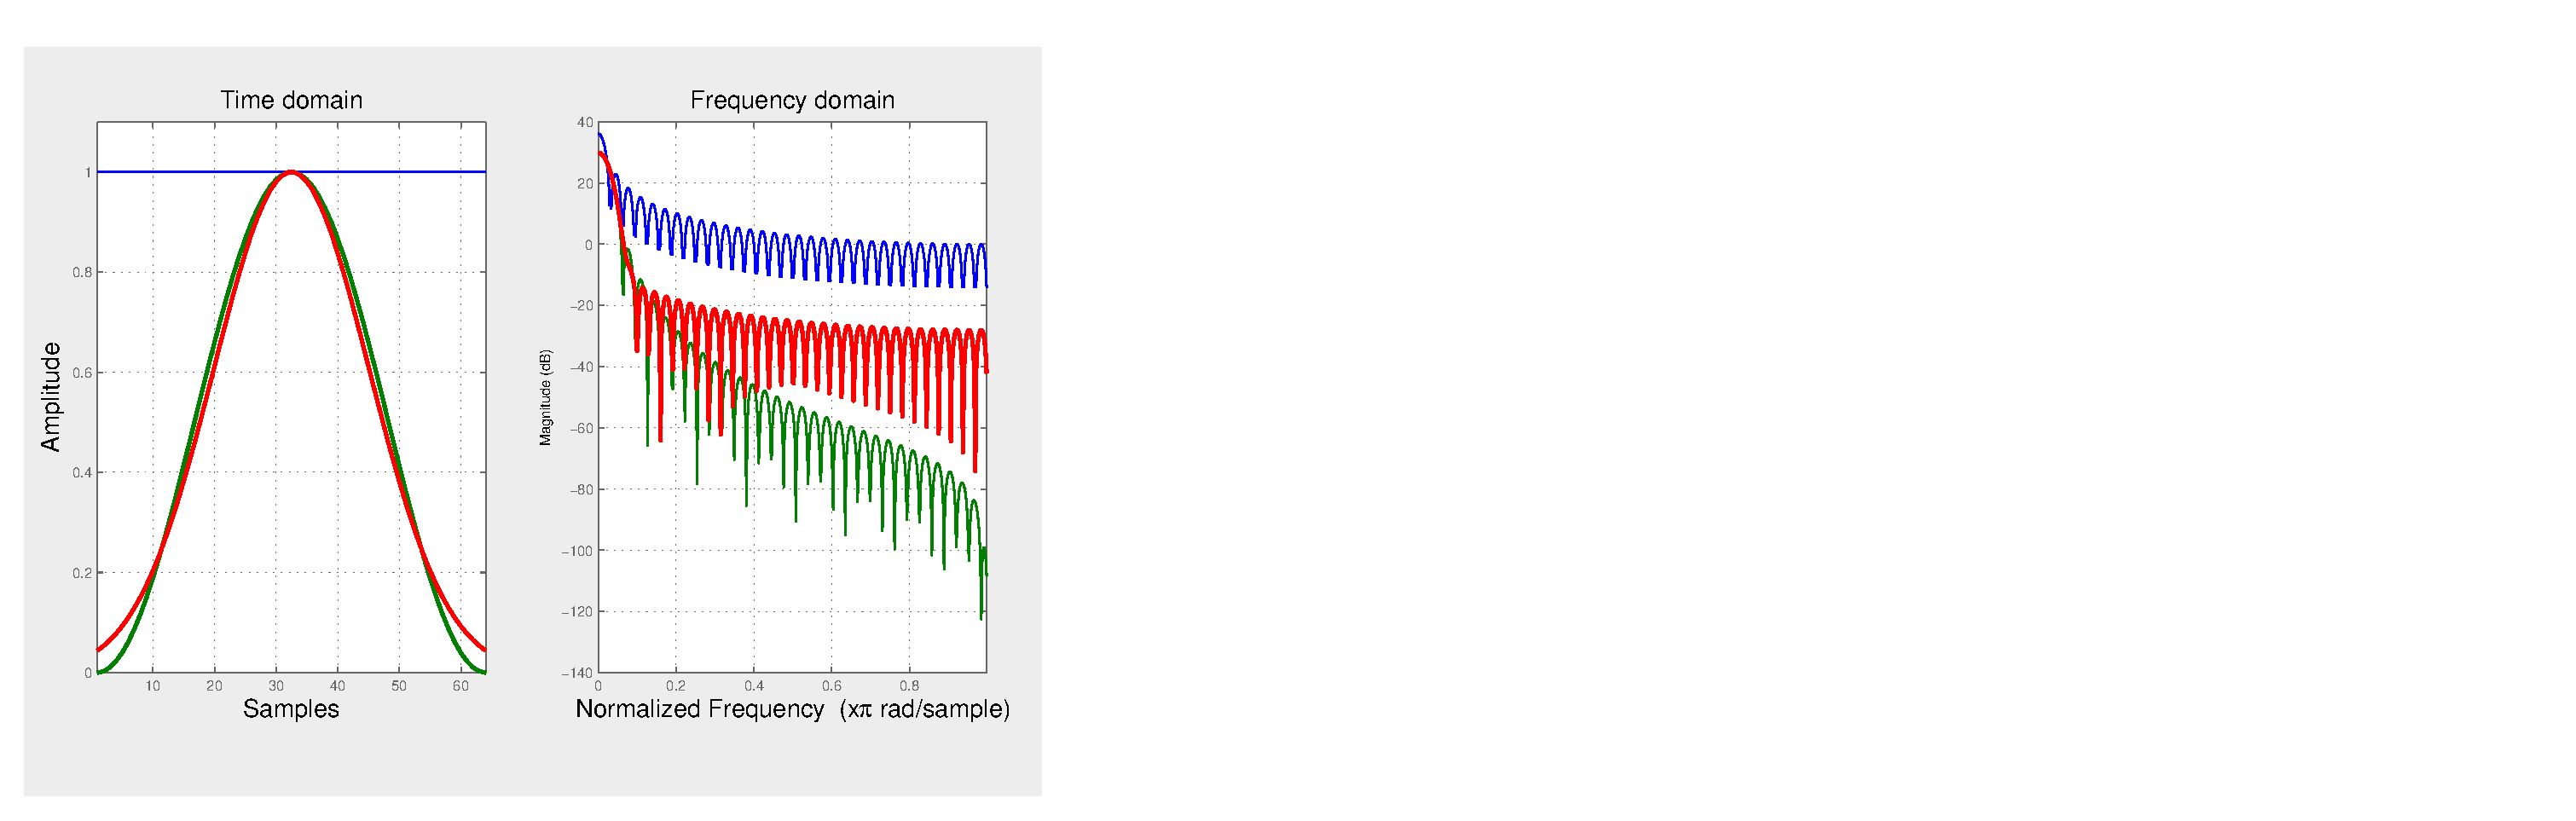
\includegraphics[scale=0.45, trim=0 0 30cm 0, clip=true]{wincomp.eps}
    \subcaption{Different windows in time and frequency domain. Blue, red and green lines correspond to the rectangular, Gaussian and Hanning window, respectively.}
    \label{fig:wc}
\end{subfigure}

\qquad
\qquad

\begin{subfigure}[H]{1\textwidth}
 \centering
    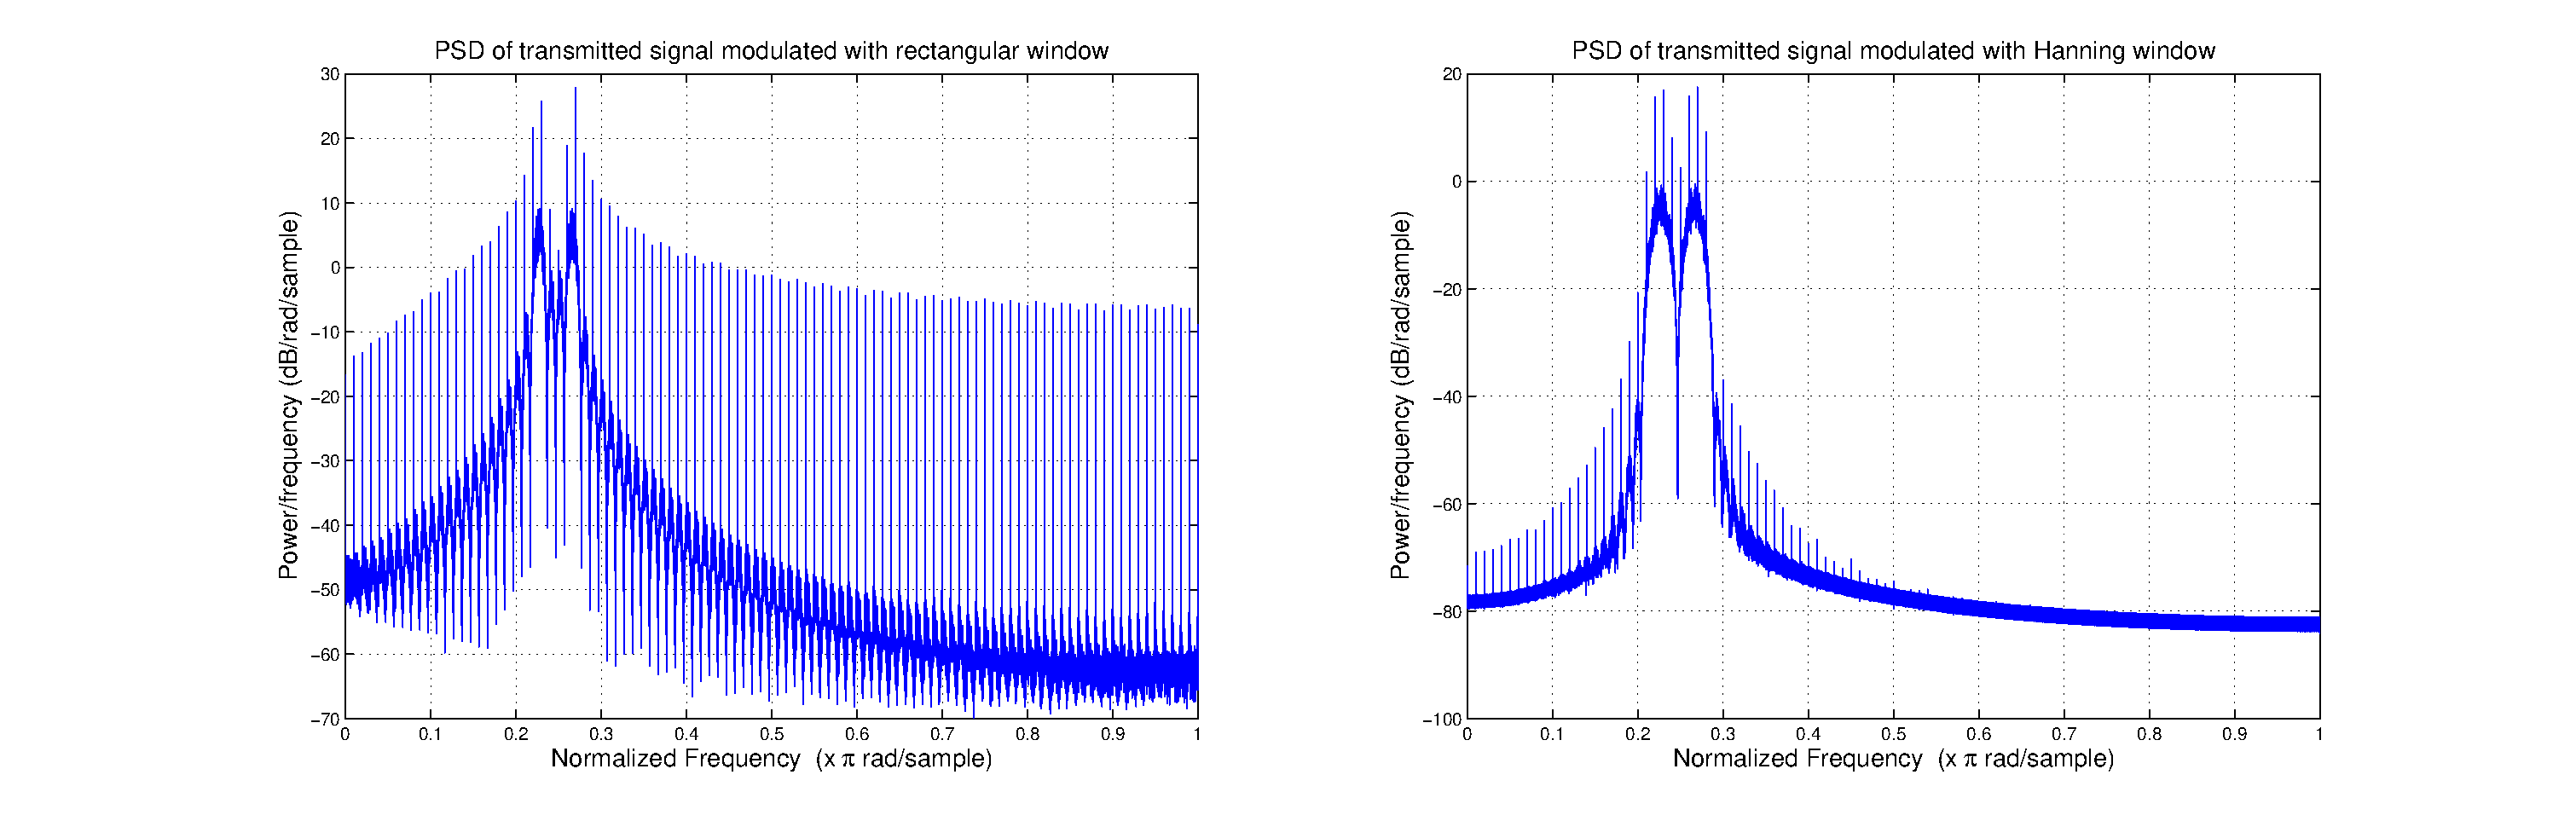
\includegraphics[scale=0.38]{txwinrectVShann.eps}
    \subcaption{PSD of the transmitted pulse using the rectangular and Hanning window for a BFSK system.}
    \label{fig:wcomp}
    
    \end{subfigure}
    
    \caption[The importance of choosing the right window for pulse shaping]{The importance of choosing the right window for pulse shaping.}
    \label{fig:main}
\end{figure}

We can see that if we make $\alpha$ large, it will result in a higher spectral efficiency. The Gaussian pulse does not satisfy the Nyquist criterion, and therefore the pulse shape introduces ISI, which increases as $\alpha$ gets larger. Therefore, improving spectral efficiency by increasing $\alpha$ leads to a higher ISI level, creating an irreducible error floor from this self-interference. The variable $\alpha$ should, hence, be chosen with care. The gaussian window effect can be seen in figure \ref{fig:gaussianalpha} and will be further developed in section \ref{sec:ts}.

 \begin{figure}[H]
  \centering
    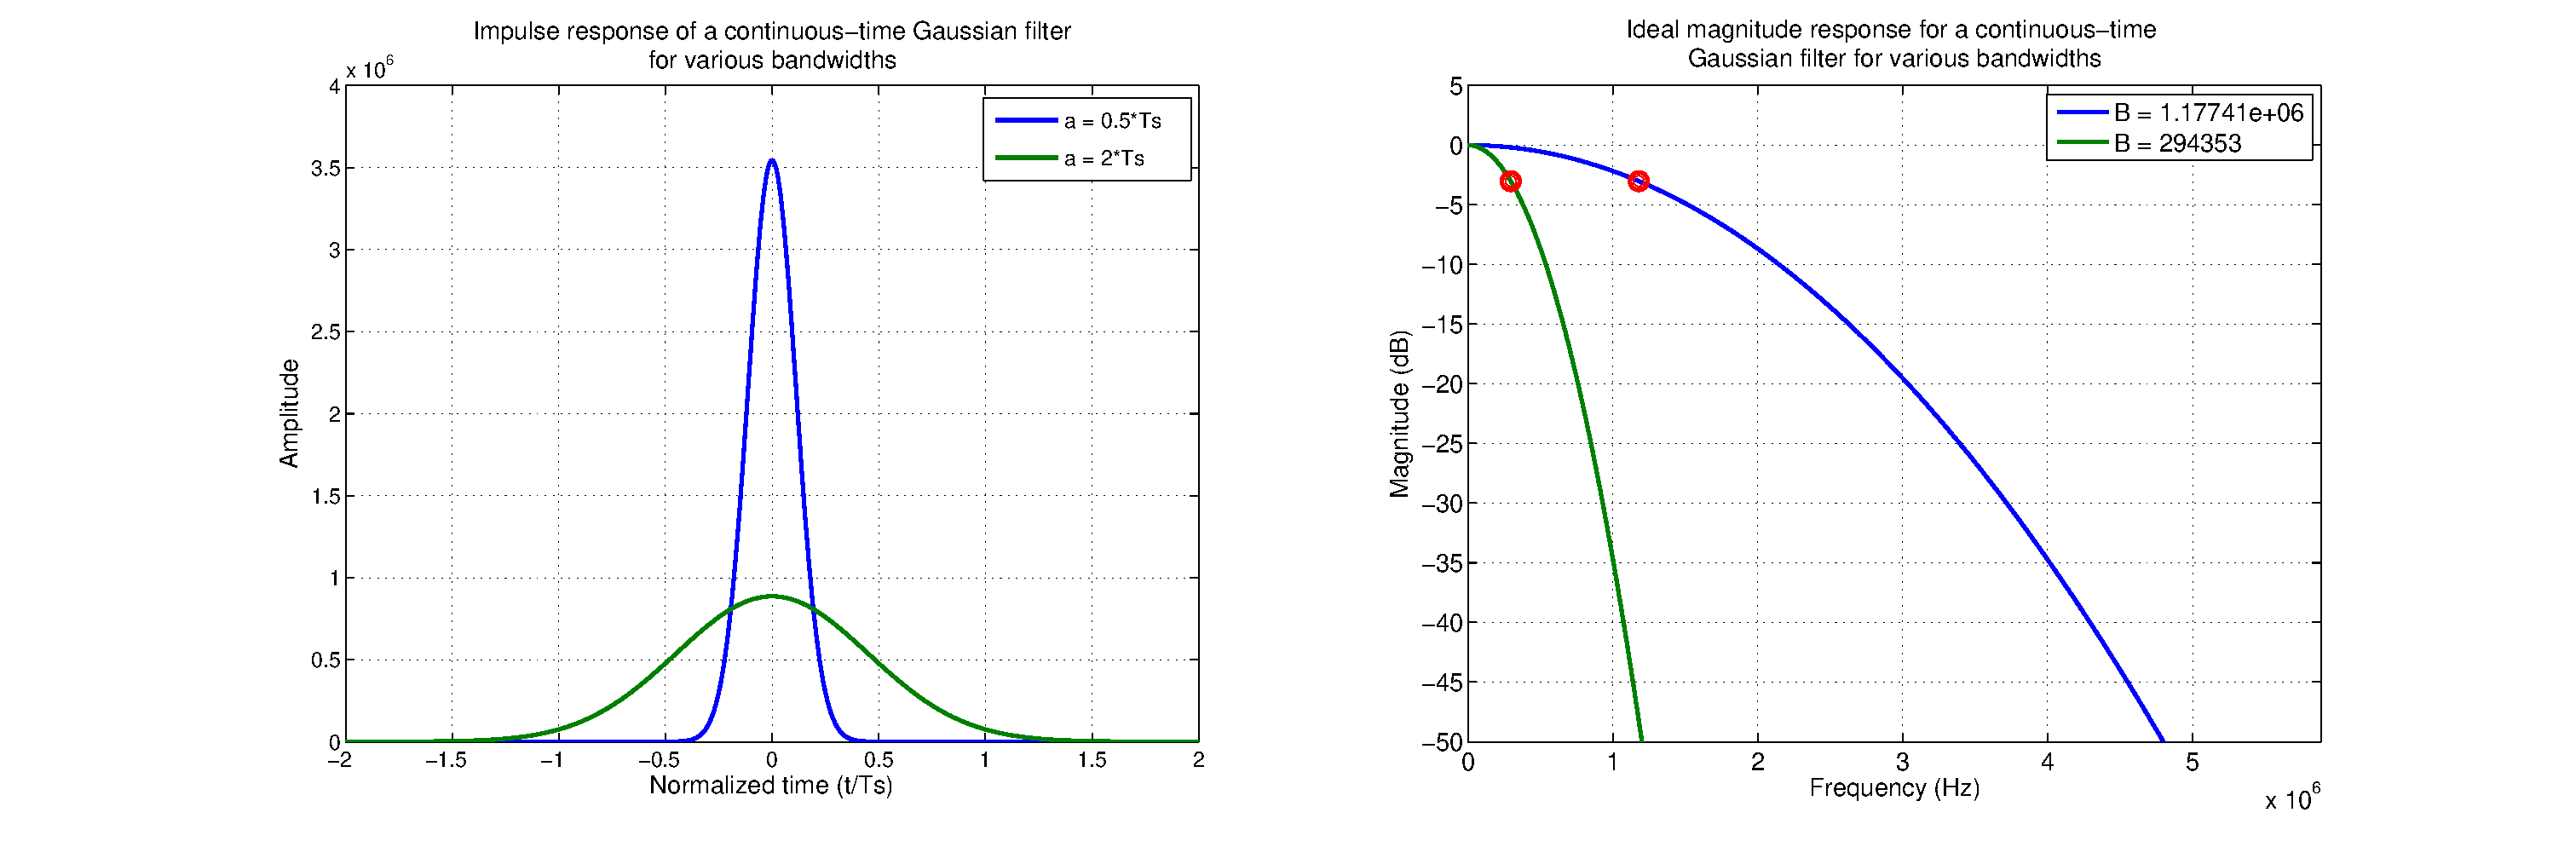
\includegraphics[width=1\textwidth]{gausswinalpha.eps}
    \caption[Ideal Gaussian filter with different values of $\alpha$]{Ideal Gaussian filter with different values of $\alpha$. The tradeoff between high spectral efficiency and reduced ISI is clear. A large $\alpha$ leads to an increased efficiency but the amplitude for $t/T_s > 1$ is not zero, leading to ISI.}
    \label{fig:gaussianalpha}
\end{figure}  

\section{Synchronisation}
\label{sec:ts}

Carrier synchronisation is an extremely important parameter for the performance of the system. Up to this point we have assumed that the receiver is perfectly synchronised with the transmitter, and the only channel impairment is AWGN. In practice, however, it is often found that there is also uncertainty due to the randomness of some signal parameters, caused by distortion in the transmission medium and hardware constraints. One of the most common random signal parameter is the carrier phase, especially for narrowband signals. A mistiming error in sampling may lead to a series of ISI components that converge and affects the overall system performance. 

There are two basic modes of synchronisation in the reception of a digitally modulated signal:
\begin{enumerate}
\item \textbf{Carrier Synchronisation.}  When coherent detection is used, knowledge of both  frequency and phase of the carrier are necessary. The process of estimating such parameters is called carrier recovery.

\item \textbf{Clock recovery.} To perform demodulation, the receiver has to know the instants of time that at which the modulation in the transmitter changes its state. In other words, the receiver has to know the starting and finishing point of the individual symbols, so that it may determine when to sample. The estimation of these times is called symbol synchronisation.
\end{enumerate}

The synchronisation algorithm is crucial for the operation of the system. Its task is to find the best sampling time for the sampling device. Ideally, the MF should be sampled such that the SNR for the decision variable is maximised. For a rectangular pulse shape, the best sampling time $t_{samp}$ is at the peaks coming out from the matched filter (see figure \ref{fig:mfpeaks}).

 \begin{figure}[H]
  \centering
    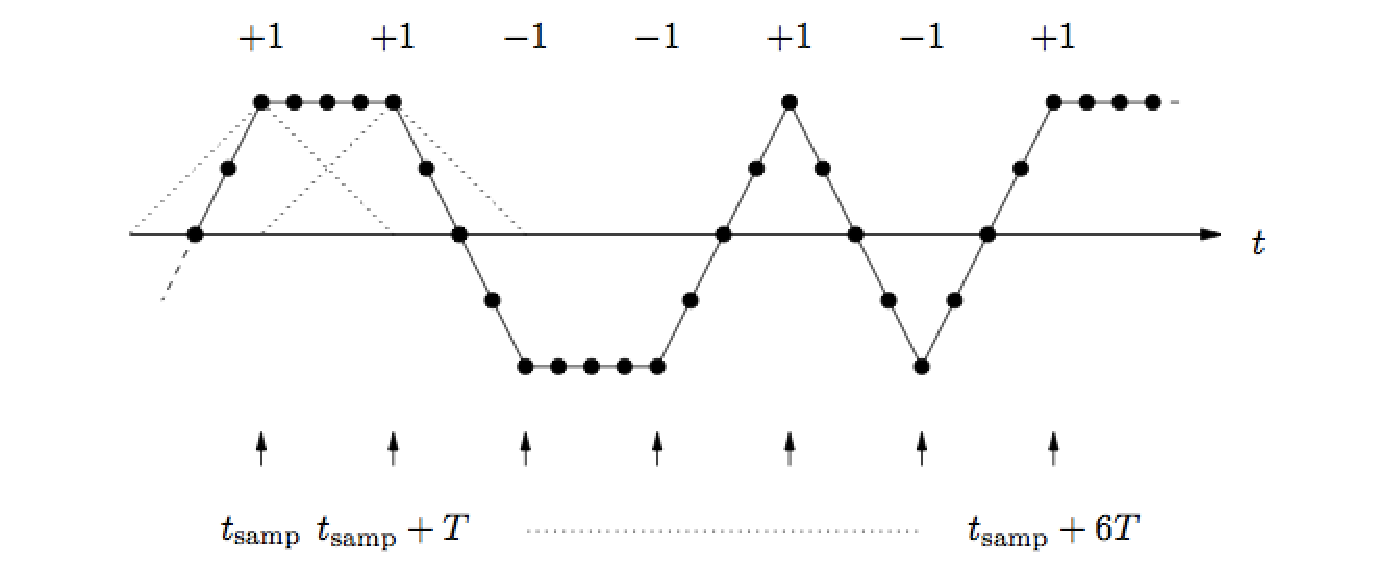
\includegraphics[width=0.7\textwidth]{mfpeaks.pdf}
    \caption[Output from the matched filter for successive signalling in absence of noise]{Output from the matched filter for successive signalling in absence of noise. The small arrows illustrate the preferred sampling instants\cite{ProjectEQ2310}.}
    \label{fig:mfpeaks}
\end{figure}

One of the most common synchronisation techniques is based on the usage of training sequences. When the signal is received, the receiver is able to identify the training sequence and recover the symbol time, by cross-correlating the samples after the matched filter with a locally generated time-shifted replica of the training sequence. This algorithm can be either applied directly to the received samples and correlating with a modulated training sequence (resolution of 1 sample but very sensitive), or applied at the symbol level (resolution of $T/Q$, where $Q$ is the number of samples per symbol). We will consider the last option to simplify. If ${\left\{ {c(n)} \right\}_{n = 0}^{L - 1}}$ is the locally generated symbol-spaced replica of the training sequence of length $L$, [$t_{start},t_{end}$] represents the search window, and $r(n)$ denotes the output from the matched filter. The timing can be found as \cite{HaykinBook}:

\begin{equation}
{t_{samp}} = \arg \mathop {\max }\limits_{{t_{samp}} \in [{t_{start}},{t_{end}}]} \left| {\sum\limits_{k = 0}^{L - 1} {r(kQ + {t_{samp}})^*c(k)} } \right|
\end{equation}

The correlation properties of the training sequence are important as they affect the estimation accuracy. Ideally, the autocorrelation function for the training sequence should be equal to a delta pulse,which means it should have a zero correlation everywhere except at lag zero. Therefore, the training sequence should be carefully designed. If, for example, the training sequence is modulated with a different frequency or pulse shape than the rest of the signal, better results for the correlation will be obtained. Such effects are depicted in figure \ref{fig:tscomp}. 

\begin{figure}[H] 
  \begin{subfigure}[b]{0.5\linewidth}
    \centering
    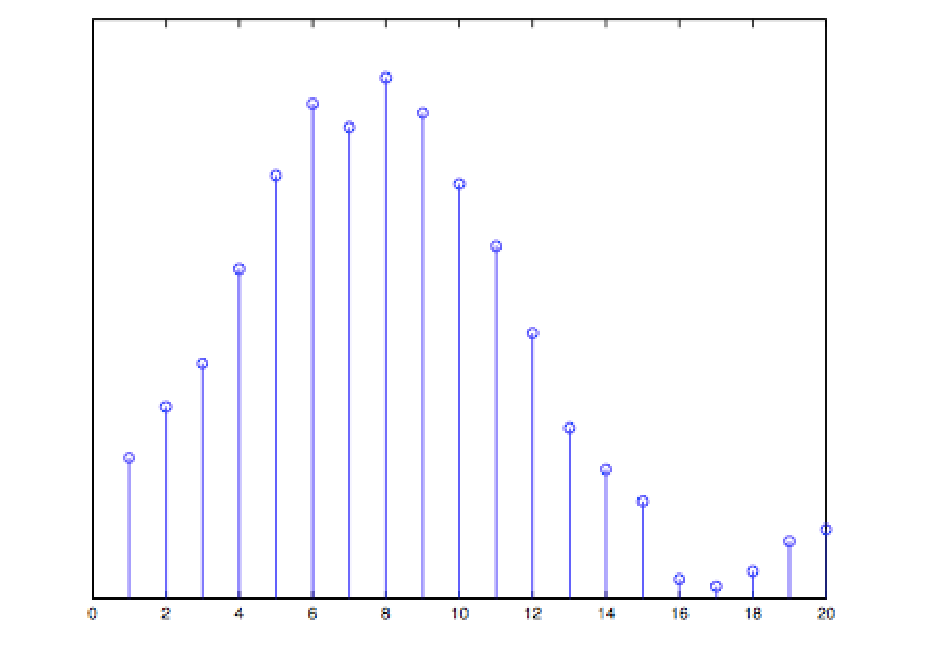
\includegraphics[width=1\linewidth]{ss.pdf} 
    \caption{Symbol spaced cross-correlation. In this example the delay is estimated to be 8 and therefore the system should be sampled at 8+kQ, k=0,1,2,..N.} 
    \label{fig:a} 
    \vspace{4ex}
  \end{subfigure}%% 
  \quad
  \begin{subfigure}[b]{0.5\linewidth}
    \centering
    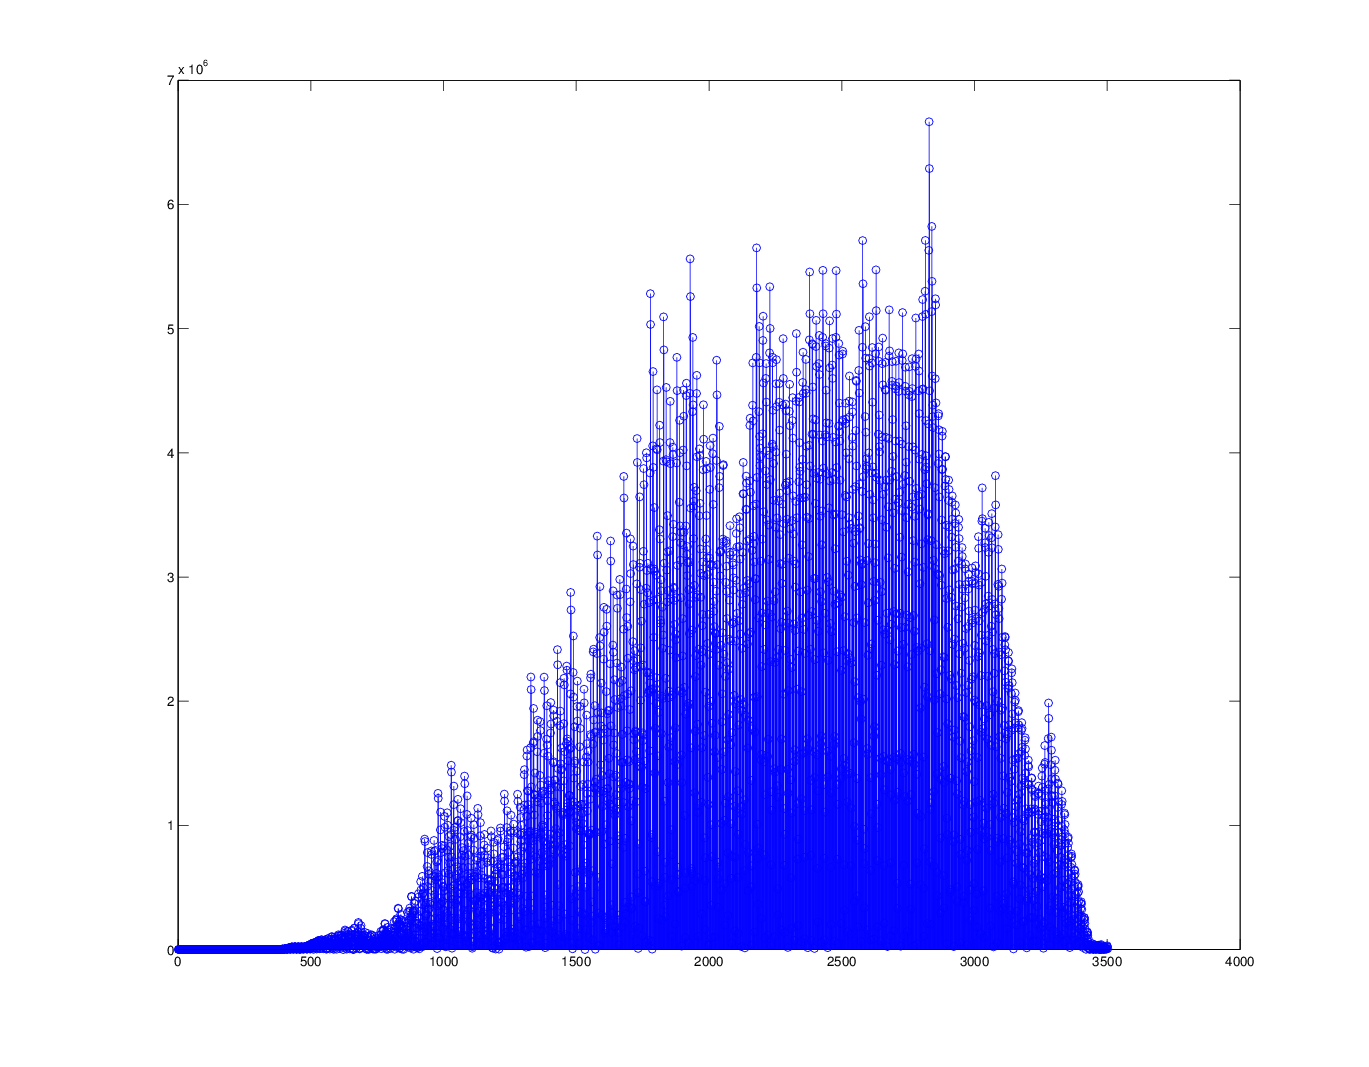
\includegraphics[width=1\linewidth]{20.png} 
    \caption{One sample resolution cross correlation with training sequence of length 20 symbols.  \\} 
    \label{fig7:b} 
    \vspace{4ex}
  \end{subfigure} 
  \quad
  \begin{subfigure}[b]{0.5\linewidth}
    \centering
    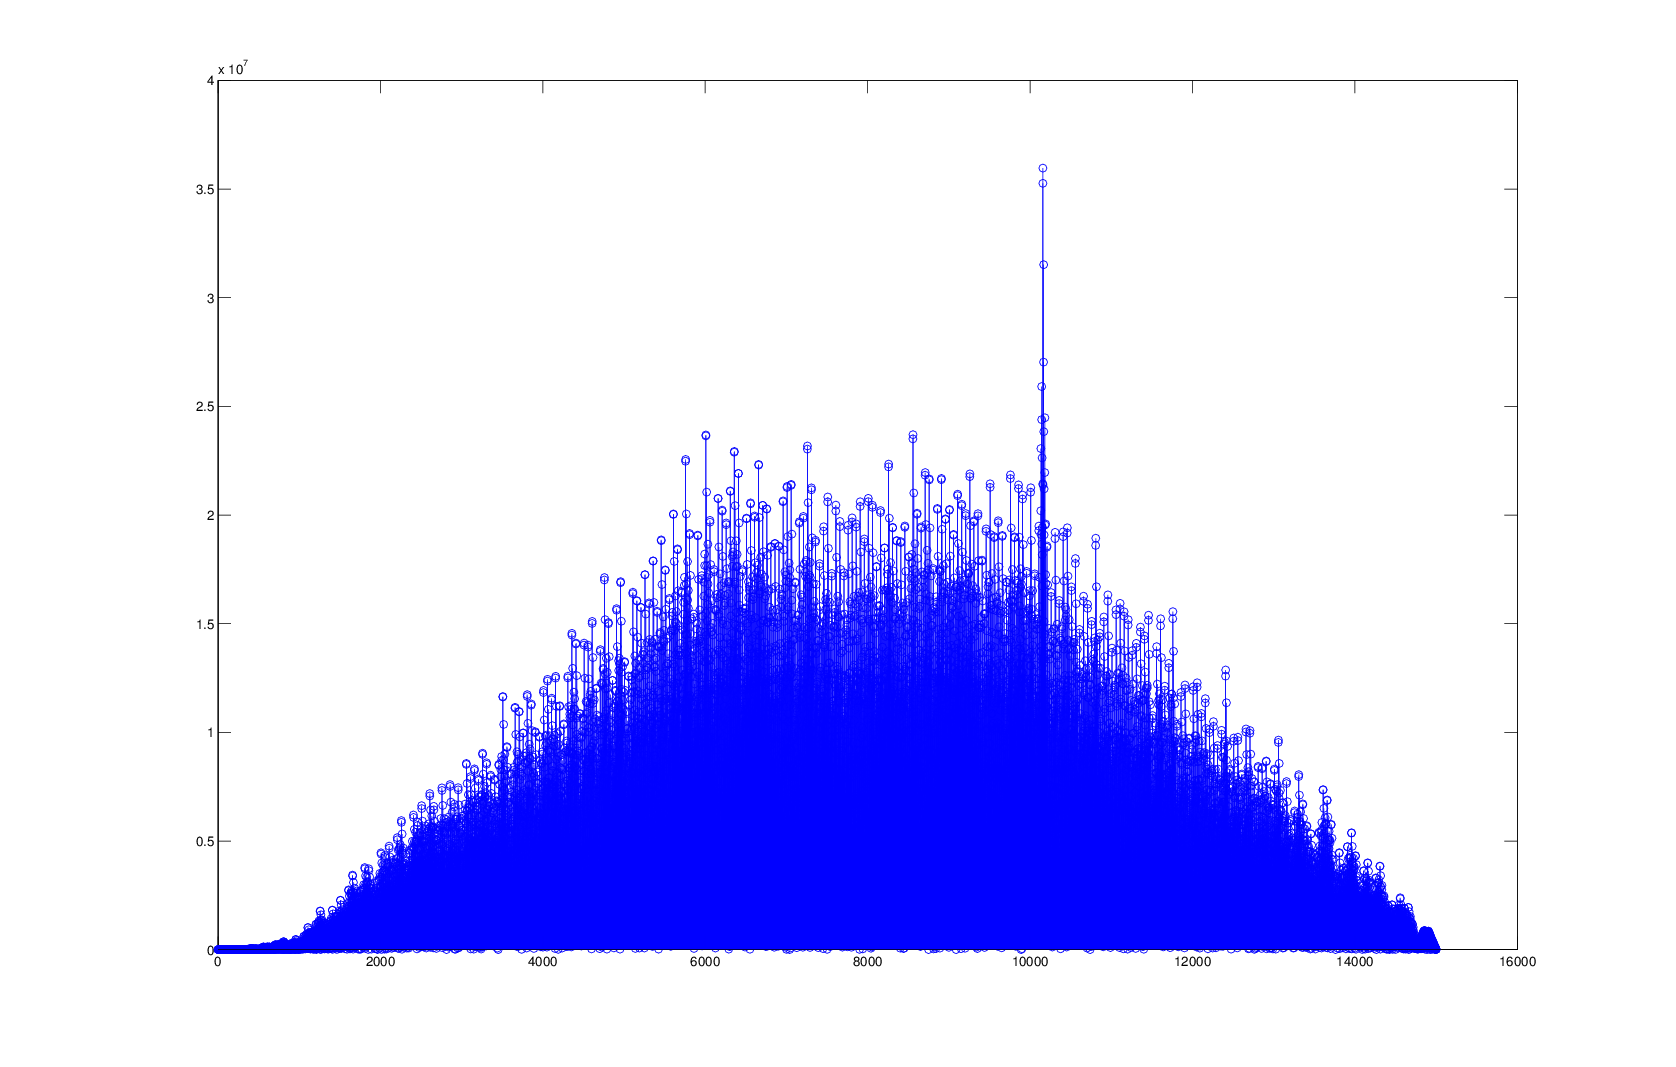
\includegraphics[width=1\linewidth]{100eq.png} 
    \caption{One sample resolution cross correlation with training sequence of length 100 symbols and equal frequency to rest of transmission.} 
    \label{fig7:c} 
  \end{subfigure}%%
  \quad
  \begin{subfigure}[b]{0.5\linewidth}
    \centering
    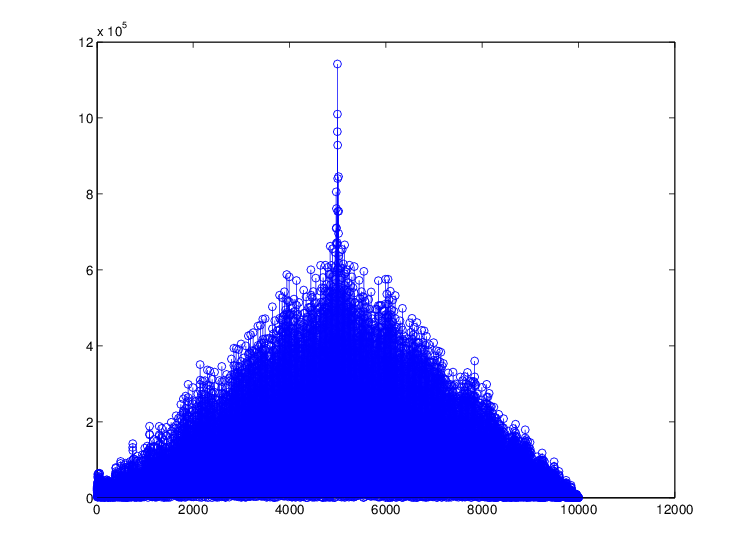
\includegraphics[width=1\linewidth]{100dif.png} 
    \caption{One sample resolution cross correlation with training sequence of length 100 symbols and different frequency to rest of transmission.} 
    \label{fig7:d} 
  \end{subfigure} 
  \caption[Training sequence algorithm/length/modulation comparison]{Training sequence algorithm/length/modulation comparison.}
  \label{fig:tscomp} 
\end{figure}

\subsection{Synchronisation in MQAM systems}
\label{subsec:MQAMsynch}
The basic operations required by an all digital MQAM receiver are illustrated in figure \ref{fig:rxMQAM}. The quadrature down-conversion and matched filter operations produce estimates of the quadrature amplitudes that are the basis of the data decisions. The role of carrier phase synchronisation is to perform the quadrature down-conversion using phase coherent replicas of the quadrature carriers.

 \begin{figure}[H]
  \centering
    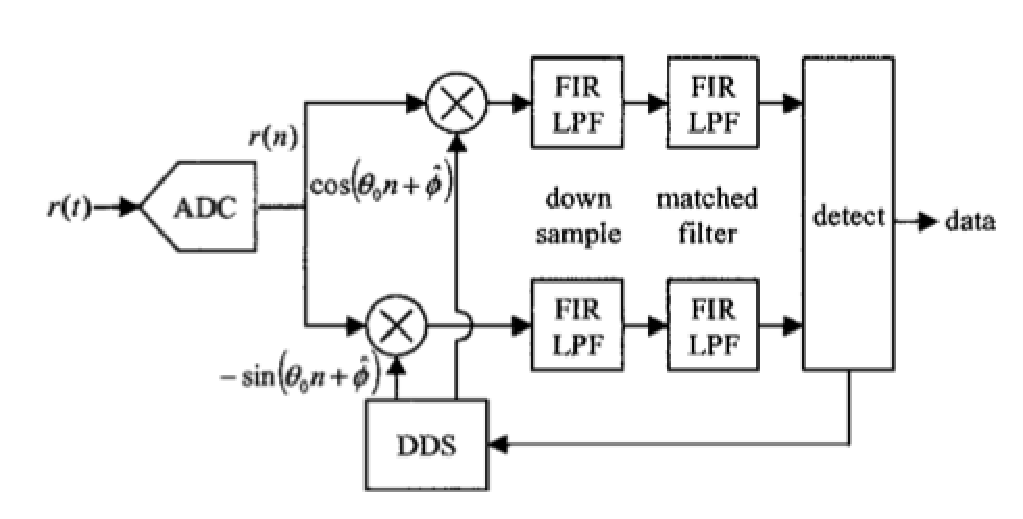
\includegraphics[width=0.6\textwidth]{rxMQAM.pdf}
    \caption[Block diagram of basic QPSK/QAM digital receiver]{Block diagram of basic QPSK/QAM digital receiver. In the digital implementation, the VCO takes the form of a direct digital synthesizer (DDS). }
    \label{fig:rxMQAM}
\end{figure}

There are many options for implementing carrier phase and frequency synchronisation in a digital communication system. At the heart of all synchronisers is the phase-locked loop (PLL). An all-digital receiver can be implemented with a digital phase-locked loop (DPLL) as shown in figure \ref{fig:DPLL}. The phase detector is implemented using the arctangent suggested by the ATAN block. The complexity of the phase detector can be reduced by computing a signal proportional to the sine of the phase difference. The phase error is computed by comparing the phase difference between the received signal $x(n) + jy(n)$ and the closest constellation point $\hat{I}(n) + j\hat{Q(n)}$ as illustrated in figure \ref{fig:PD1}.

 \begin{figure}[H]
 \centering
\begin{subfigure}{0.5\textwidth}
 \centering
    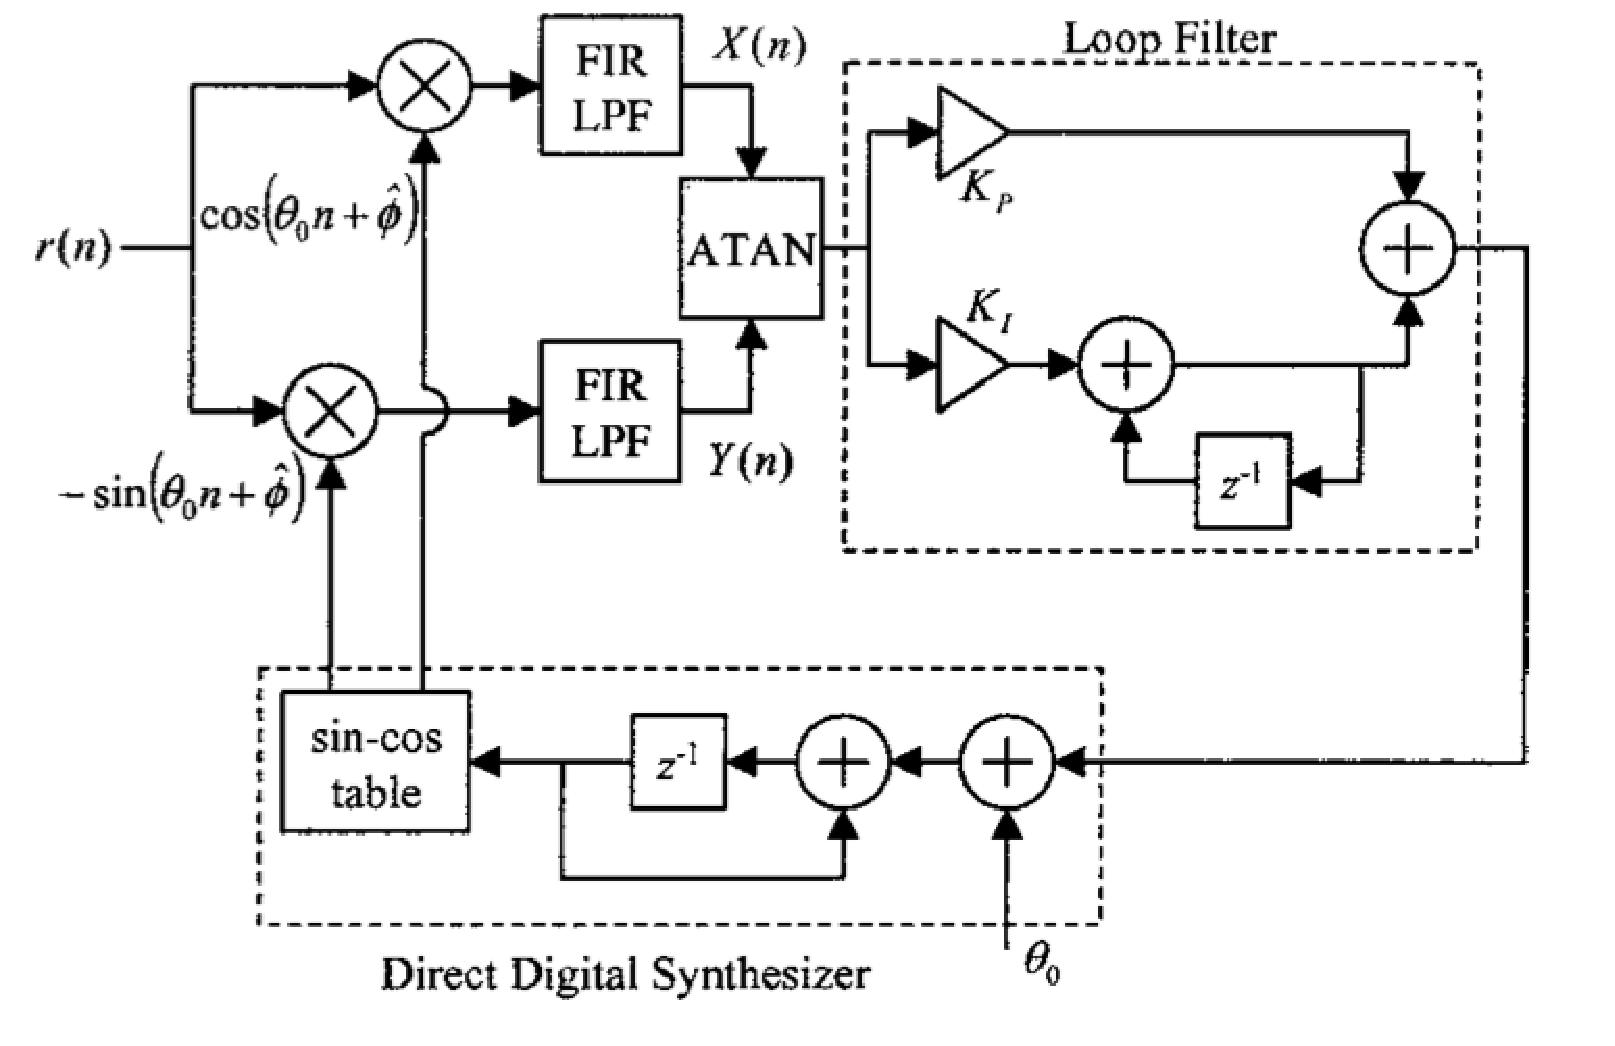
\includegraphics[width=0.9\linewidth]{DPLL.pdf}
    \caption{Digital phase locked loop for carrier phase \\ synchronisation. \\}
    \label{fig:DPLL}
\end{subfigure}%
\begin{subfigure}{0.5\textwidth}
 \centering
    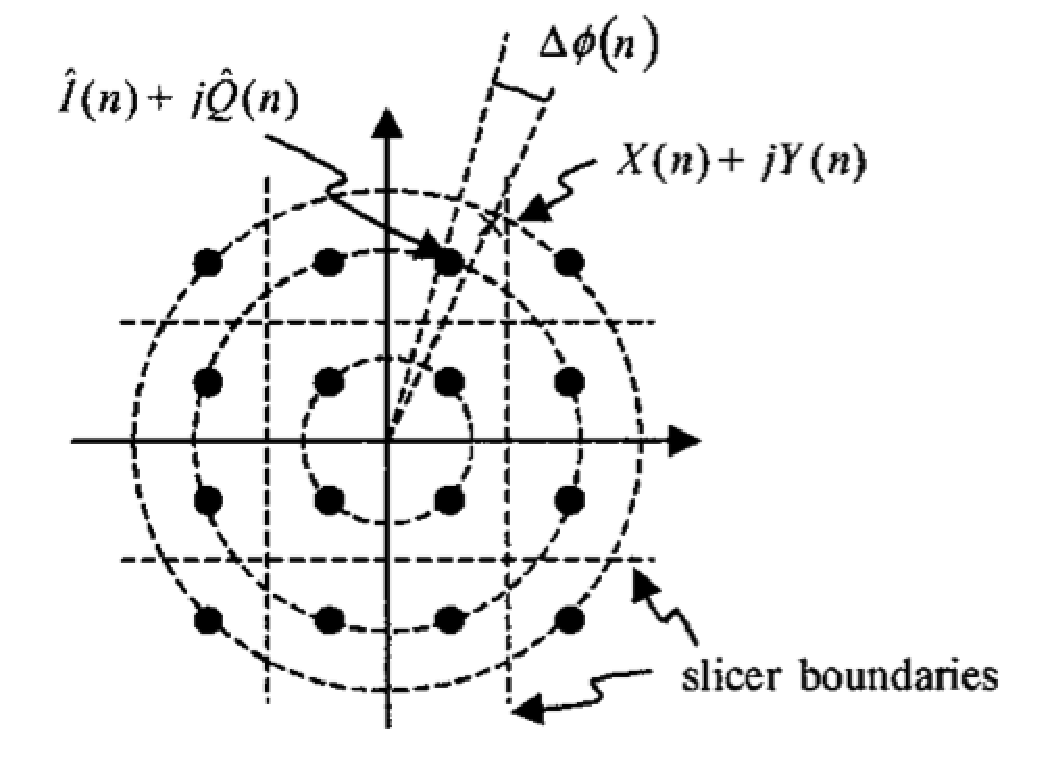
\includegraphics[width=0.7\linewidth]{PD.pdf}
    \caption{16-QAM constellation with decision boundaries and phase error.}
    \label{fig:PD1}
    \end{subfigure}
    \caption[Carrier phase estimation diagrams]{Carrier phase estimation diagrams\label{CarrierSynchPaper}.}
    \label{fig:carrierphase}
\end{figure}

The initial phase estimation can be done using the procedure described above, taking into account the training sequence is known at transmitter and receiver. Let's assume the channel causes a rotation of $\varphi$ to the symbol constellation. The value of $\varphi$ can be computed using the element-wise multiplication of the received symbol with the complex conjugate of a modulated training sequence replica and then averaging over the sequence. In other words, if ${\left\{ {\tilde r(n)} \right\}_{n = 0}^{L - 1}}$ denotes the $L$ received symbols and ${\left\{ {c(n)} \right\}_{n = 0}^{L - 1}}$ the local replica of the complex training sequence, an estimate of the phase offset can be obtained as \cite{ProjectEQ2310}:

\begin{equation}
\hat \varphi  = \frac{1}{L}\sum\limits_{k=0}^{L - 1} {\arg (\tilde r(k)c(k)^*)}
\end{equation}

The longer the training sequence, the better the phase estimate as the influence from the noise decreases. On the other hand, a long training sequence, reduces the amount of payload that can be transmitted during a given time.

\subsection{Phase rotation}
\label{subsec:Phase rotation}
Another problem that may be faced in a real implementation is the Doppler shift introduced during the transmission, which causes the constellation to rotate further more (than the initial rotation). This frequency offset could be the result of relative motion between the transmitter and receiver, as would be the case with a mobile terminal travelling away or towards a receiver. It could also be attributed to small frequency variations of the various synthesisers in both the transmitter and receiver, which are functions of time and temperature. In order to overcome this problem, at least two approaches are possible. The first is to introduce a training sequence in the data so that a new phase estimation can be computed, resulting in a lower rate. The other solution, is to divide the decisions into various small blocks in which the offset does not influence the decision, estimate the phase rotation from the nearest points and rotate the constellation for future decisions. In this way, the rate is not affected but a correct decision in each block is assumed. The frequency offset effect can be seen in figure \ref{fig:phaseoff}, where a 16-QAM signal of 5 seconds is transmitted. 


 \begin{figure}[H]
 \centering
\begin{subfigure}{0.32\textwidth}
 \centering
    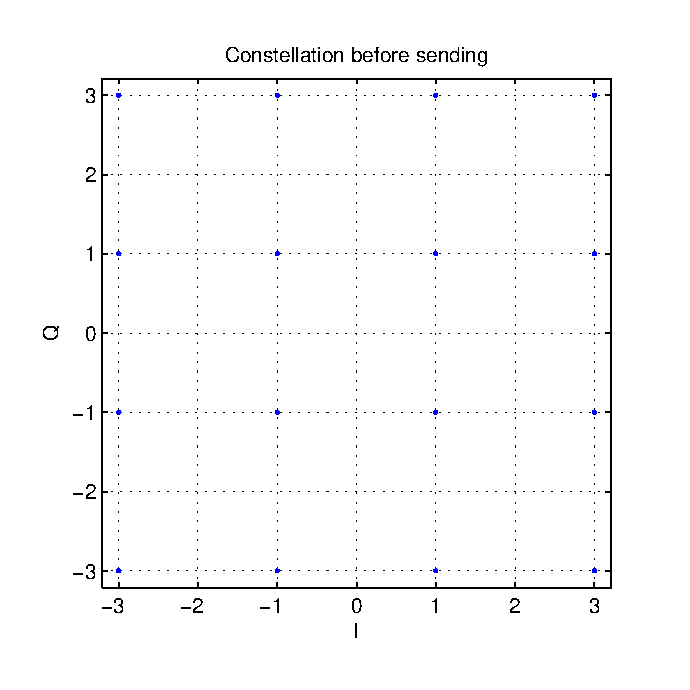
\includegraphics[width=0.8\linewidth]{tx_const.eps}
    \caption{Transmitted constellation.}
    \label{fig:DPLL2}
\end{subfigure}%
\begin{subfigure}{0.32\textwidth}
 \centering
    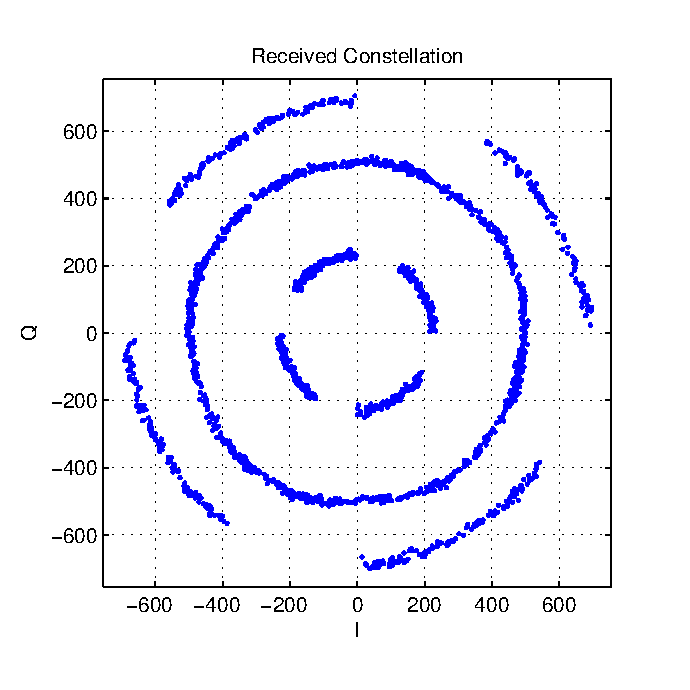
\includegraphics[width=0.8\linewidth]{rx_const.eps}
    \caption{Received constellation.}
    \label{fig:PD2}
    \end{subfigure}
    \begin{subfigure}{0.32\textwidth}
 \centering
    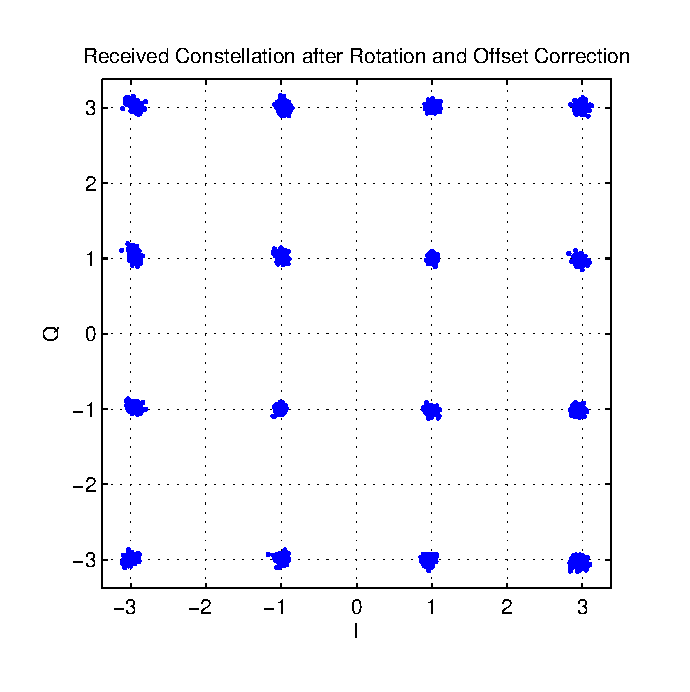
\includegraphics[width=0.9\linewidth]{rx_const_after.eps}
    \caption{Received constellation after phase correction.}
    \label{fig:PD3}
    \end{subfigure}
    \caption[Example of frequency offset in a 16-QAM constellation]{Example of frequency offset in a 16-QAM constellation with decision boundaries.  }
    \label{fig:phaseoff}
\end{figure}

%By trying different time-shifts in steps of $\frac{T}{Q}$, where $Q$ is the number of samples per symbol, the symbol timing can be found with a resolution of  $\frac{T}{Q}$.



\section{Channel Equalisation}
\label{sec:chanEQ}
The performance of a digital system is constrained by the type of channel in which the implementation is done. For our case, in theory, we have a nearly-ideal low-pass channel with low noise variance and limited up to about 20 kHz. However, the phone's audio card introduce non-linear distortion that affects the signal output and causes attenuation around 6kHz (see figure \ref{fig:channelresp}). This can both cause ISI as a result of the channel impulse response, as well as distortion of the signal spectrum. Thus, to improve the performance of our system, we can use channel equalisation techniques to reduce the ISI, and allow a better recovery of the transmitted symbols. The equalisation method will depended on the type of modulation scheme, as well as the channel response. For the case of FSK, the amplitude distortion will not affect at a great extent, but for M-QAM we shall compensate such distortion without affecting the carrier phase. In addition, we can expect a non-varying channel that allows the usage of parametric digital filters.  

\begin{figure}[H]
\centering
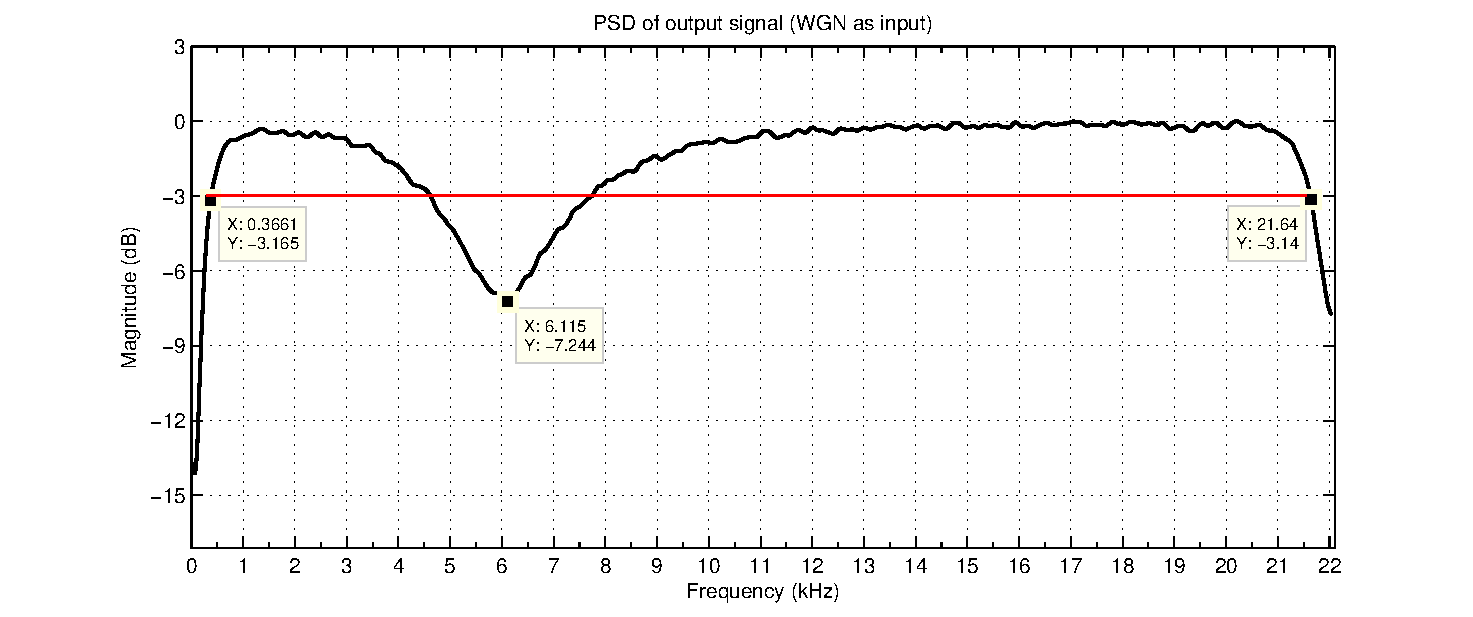
\includegraphics[width=0.7\textwidth]{ChannelResponse.pdf}
\caption[Estimated channel frequency response to WGN]{Estimated channel frequency response to WGN. The measured 3dB bandwidth is 21.27kHz.}
\label{fig:channelresp}
\end{figure}


\subsection{IIR filters}
Infinite Impulse Response (IIR) filters are recursive structures of a discrete LTI system that can be defined generically in the following form \cite{DSPDiniz}:

\begin{equation}\label{Eq:IIR}
H\left( z \right) = \frac{{\sum\limits_{\ell  = 0}^M {{b_\ell }{z^{ - \ell }}} }}{{1 + \sum\limits_{\ell = 1}^N {{a_\ell }{z^{ - \ell }}} }}.
\end{equation}

 The rational transfer function described in equation \ref{Eq:IIR} implies that the system will have an infinite response, when feeding it with a Dirac impulse. The coefficients from the numerator polynomial correspond to the feed-forward terms, and the ones from the denominator, correspond to the feedback terms (see figure \ref{fig:IIRimpl}). IIR filters can be represented in several forms or realisations, however, we generally have to base our design in a given set of initial parameters, such as pass-band, stop-band, ripple, or roll-off. Amongst the main advantages of these kind of filters, we have that they can efficiently meet a given specification with relative low complexity and efficiency.  In general, this  computational efficiency is rather large compared to FIR filters, described in the next section.
 
  \begin{figure}[H]
   \centering
     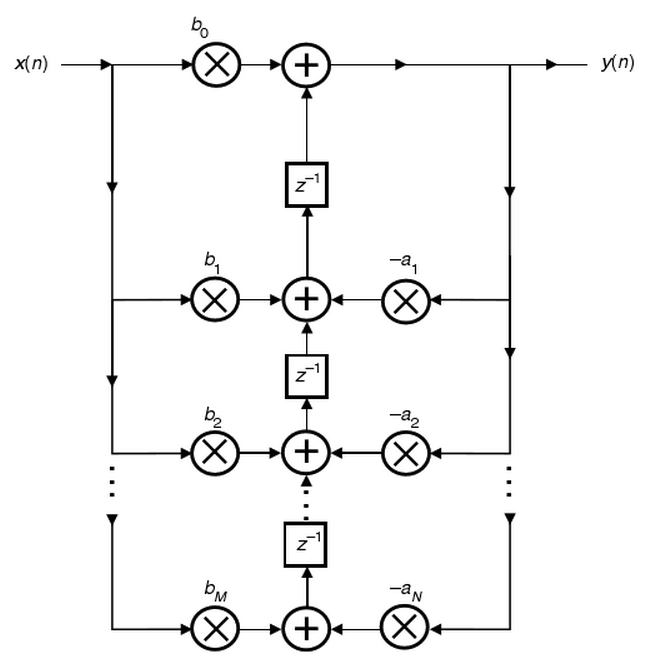
\includegraphics[width=0.5\textwidth]{IIRfilter.png}
     \caption[Shift register implementation of an IIR filter]{Shift register implementation of an IIR filter (Type 2 canonic direct form)\cite{DSPDiniz}.}
     \label{fig:IIRimpl}
 \end{figure}  

\subsection{FIR filters}
Finite Impulse Response (FIR) filters are non-recursive linear systems that are also widely used in signal processing because of their stability and relative simple implementation. Their transfer function only contains feed-forward terms with coefficients $b_\ell$ directly related with the filter impulse response as follows\cite{DSPDiniz}: 
\begin{equation}\label{Eq: FIR}
H\left( z \right) = \sum\limits_{\ell  = 0}^M {{b_\ell }{z^{ - \ell }}}=\sum\limits_{\ell  = 0}^M {{h_\ell }{z^{ - \ell }}}
\end{equation}

As seen in equation \ref{Eq: FIR}, these kind of filters can be easily designed when we compute the coefficients that characterise the channel impulse response. FIR filters may also have good characteristics compared with the case of IIR filters, such as linear phase and stability. The biggest problem that we may face when using such designs, is that we need to have a relative high order compared to the case of a similar IIR filter. This adds additional delay to the signal processing and slows down the system. The shift register implementation of a typical FIR filter is depicted in figure \ref{fig:FIRfilter}.
 
  \begin{figure}[H]
   \centering
     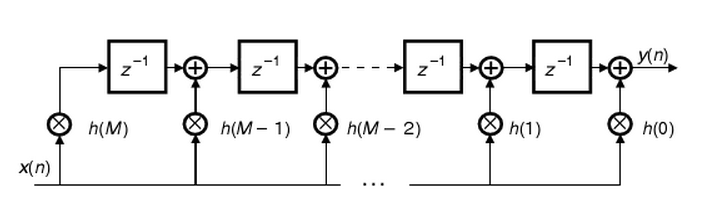
\includegraphics[width=0.8\textwidth]{FIRfilter.png}
     \caption[Shift register implementation for a FIR filter]{Shift register implementation for a FIR filter (Direct form)\cite{DSPDiniz}.}
     \label{fig:FIRfilter}
 \end{figure}  

\section{Channel Coding}
\label{sec:channcod}
The digital signal is subject to diverse perturbations that provoke distortion throughout a non-ideal channel. It is also likely that such distortion  cannot be fully compensated with an Equaliser or filter, thus, error correcting codes may be implemented. Our channel is bandwidth and power limited, these two parameters together with the noise spectral density will determine the bit-error rate (BER)\cite{HaykinBook}. In our system, the channel impairments result in frequency distortion and ISI. An orthogonal  modulation scheme may be able to mitigate such perturbations, however, it is still likely to have errors at the receiver that can be corrected by adding redundancy to the transmitted signal. This implies that the overall information rate will be decreased when using overheads such as training sequences or error correcting codes.
 
 There are two basic schemes to implement error correction capabilities into our system: error detection/retransmission, and forward error correction (FEC)\cite{SklarBook}. In the first scheme, the receiver terminal asks the transmitter to retransmit the data if it detects an error. When FEC is used, the receiver tries to recover the signal using the added redundancy. Hence, the detection and retransmission scheme requires a two-way communication contrary to the case of using forward error correction. We will focus on the last scheme since our system is only able to send data in one direction. In this fashion, the information message shall be encoded before it is modulated and sent trough the channel (figure \ref{fig:ChanCodTX}). The reverse process is done at the receiver, as shown in figure \ref{fig:ChanCodRX}. The most widely used codes are linear codes, which can be classified into two general forms: block codes and convolutional codes. One of the principal differences between the two groups is that the encoder for the case of convolutional codes has memory elements.
 
  \begin{figure}[H]
  \centering
 	\begin{subfigure}[H]{1\textwidth}
  \centering
     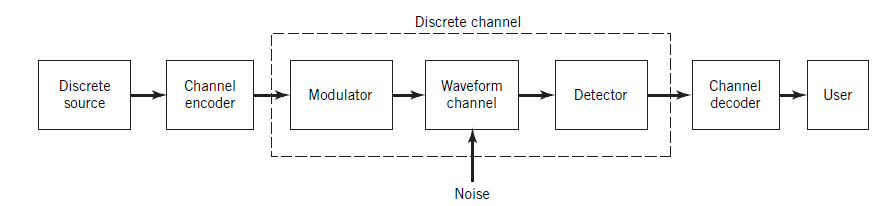
\includegraphics[width=0.8\textwidth]{chancodtx.PNG}
     \subcaption{Transmitter with channel encoder.}
     \label{fig:ChanCodTX}
 
 	\end{subfigure}
 	\quad
 
 	\begin{subfigure}[H]{1\textwidth}
  	\centering
	     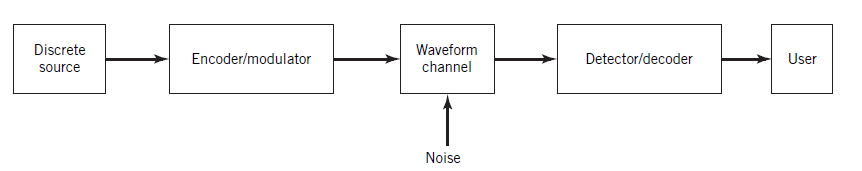
\includegraphics[width=0.8\textwidth]{chancodrx.PNG}
     \subcaption{Receiver with channel decoder.}
     \label{fig:ChanCodRX}
  	\end{subfigure}
     \caption[Digital communication system with forward error correction]{Digital communication system with forward error correction\cite{HaykinBook}.}
     \label{fig:ChanCoding}
 \end{figure}
 
 
 \subsection{Block Codes} 
 In general, binary block codes  are parity check codes that can be characterised by the parameters $(n,k)$. In this notation, $n$ represents the number of encoded bits, and $k$ is the number of information bits. We can define the ratio $k/n$ as the rate of the code. The mapping from the set of $M=2^k$ information sequences of length $k$ can be represented by a $k\times n$ generator matrix, conventionally denoted as $\bf{G}$. Therefore, we can write the encoded sequence $\bf{c}$ (of length $n$) in matrix form as follows:
\begin{equation}
 {\bf{c}} ={{\bf{u}}}{\bf{G}}
 \end{equation}
The vector  $\bf{u}$ denotes the information sequence (of length $k$), and the row vectors of $\bf{G}$ determine the basis of a non-unique vector space. When $\bf{G}$ has the form ${\bf{G = }}\left[ {{{\bf{I}}_k}{\bf{|P}}} \right]$, we could find a parity matrix ${\bf{H = }}\left[ {{{\bf{I}}_{n - k}}{\bf{|}}{{\bf{P}}^T}} \right]$ that would lead us to decode the original data\cite{SklarBook}. These codes are mainly used for hard-decision decoding with a built-in algebraic structure based in the properties of finite fields. There exist a variety of block codes termed as Long-Density Parity-Check Codes (LDPC) that can achieve performance very close to the channel capacity.  


 \subsection{Convolutional Codes}
 Convolutional codes are linear codes which are generated by passing the information sequence through a shift register. They can be described by some encoding function $G({\bf{u}})$, such that ${\bf{c}}=G({\bf{u}})$. The encoder outputs at any given time will only depend on the inputs. The number of output bits for each $k$-bit input is a sequence of length $n$. We also need to define the parameter $K$ as the code constraint length, which represents the number of stages (of $k$-bits) in the encoder. 

One possible method to describe a convolutional code is by giving its generator matrix. Nevertheless, such matrix would be semi-infinite since the input sequence can have any arbitrary length\cite{Proakis}. A different method to describe a convolutional code, comes from the fact that each of the output sequences, can be interpreted as the convolution of the input sequence with a binary filter, defined by some ``impulse response" or, generator polynomial\footnote{Since we are using binary arithmetic operations, the polinomyals are typically given in octal form.}, denoting the links between the input, output and shift registers. A typical shift register implementation of such codes is shown in figure \ref{fig:convCodeImp}.
 
 
  \begin{figure}[H]
   \centering
     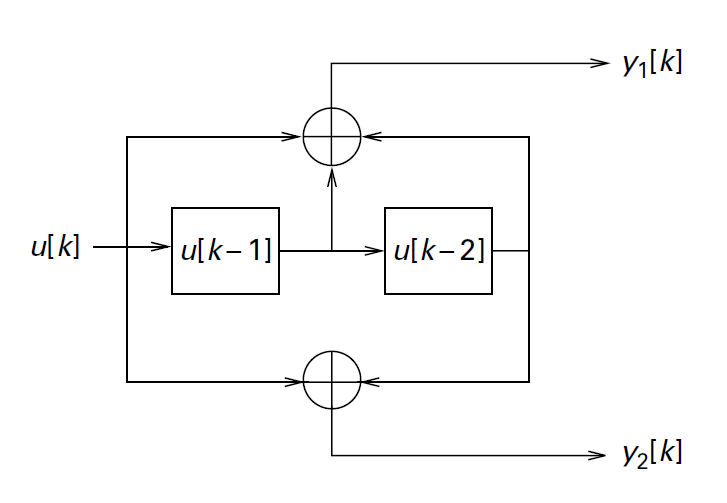
\includegraphics[width=0.4\textwidth]{convCode.PNG}
     \caption[Shift register implementation of convolutional encoder]{Shift register implementation of convolutional encoder with generator polynomials $[7,5]$ \cite{Madhow}.}
     \label{fig:convCodeImp}
 \end{figure}  
 
 Convolutional codes may be used as a building block for turbo-codes, which can perform very close to the channel capacity, as well as LDPC codes do. The major disadvantages for those two approaches are the relative complexity and hard processing that are required to achieve a good performance. 

% % % % % % % % % % % % % % % % % % % % % % % % % % % % % % % % % % % % %
% % % % % % % % % % % % % % % % % % % % % % % % % % % % % % % % % % % % %




\chapter{Android Prototype}

Our aim is to build a full digital communication system that uses a pair of Android phones as terminals and communicate them with an audio cable that will act as the channel together with the sound card of the device. The implementation consists in two modes: off-line and real-time. We define off-line and real-time as follows. Assume that the file size is $F$ (bits) and the data-rate $C$ (bps). The transmitter is allowed to transmit signals during $F/C$ seconds. In off-line mode the receiver should be able to decode the signal within 100 seconds using the received signal downloaded from the phone and process it with MATLAB. In real-time the receiver should finish decoding within $0.5\times F/C$ seconds after the transmitter has finished sending the data. The file should have size between 100 and 1000 bytes \cite{EQ2440ProjectDescription}.

The advanced specifications requires a data-rate of 32 kbps in real-time and 128kbps in off-line mode. In real-time the system should be able to transmit file sizes up to at least 10kB.


\section{Software and Hardware}


\textbf{Used Hardware}
\begin{itemize}
\item Samsung Galaxy S3 (GT-i9300) phones with Android 4.2.1.
\item 3.5mm audio cable {\color{Black}\footnote{The audio cable is modified so as to have the audio input in one end linked to the audio output in the other extreme.}}.
\item Dell PC's with Windows 7.
\\

\textbf{Used Software}
\item MATLAB R2013b 
\item Android Developer Tools IDE (Eclipse) with  API for Android 4.1.2. 
\item Git source code manager software for Windows.

\end{itemize}


\section{Android FrameWork}

Framework is an Android application developed by Martin Ohlsson and Per Zetterberg which has been designed as the groundwork for our project and to support our software implementation in real-time. The JAVA based implementation contains functions that enable the control and initiation of various sensors of the android phone (e.g. microphone, camera, speakers, among others.). In addition it has an embedded  Guided User Interface (GUI) and a number of valuable built-in features allowing us to focus more in the communication system implementation instead of software designing. \\
The file StudentCode.java is included in the FrameWork which is the main file modified and worked in. \textcolor{red}{[Some of the things that were added to StudentCode to make it work]}.\\

Figure \ref{fig:FrameWorkPicture} illustrates a diagram of the complete FrameWork and the connections between the main files. In the boxes some of the main function names that belong to that java file are shown. For example the file Complex.java \cite{ComplexJavaRef} allows us to use and handle complex numbers in the program. 




 \begin{figure}[H]
  \centering
    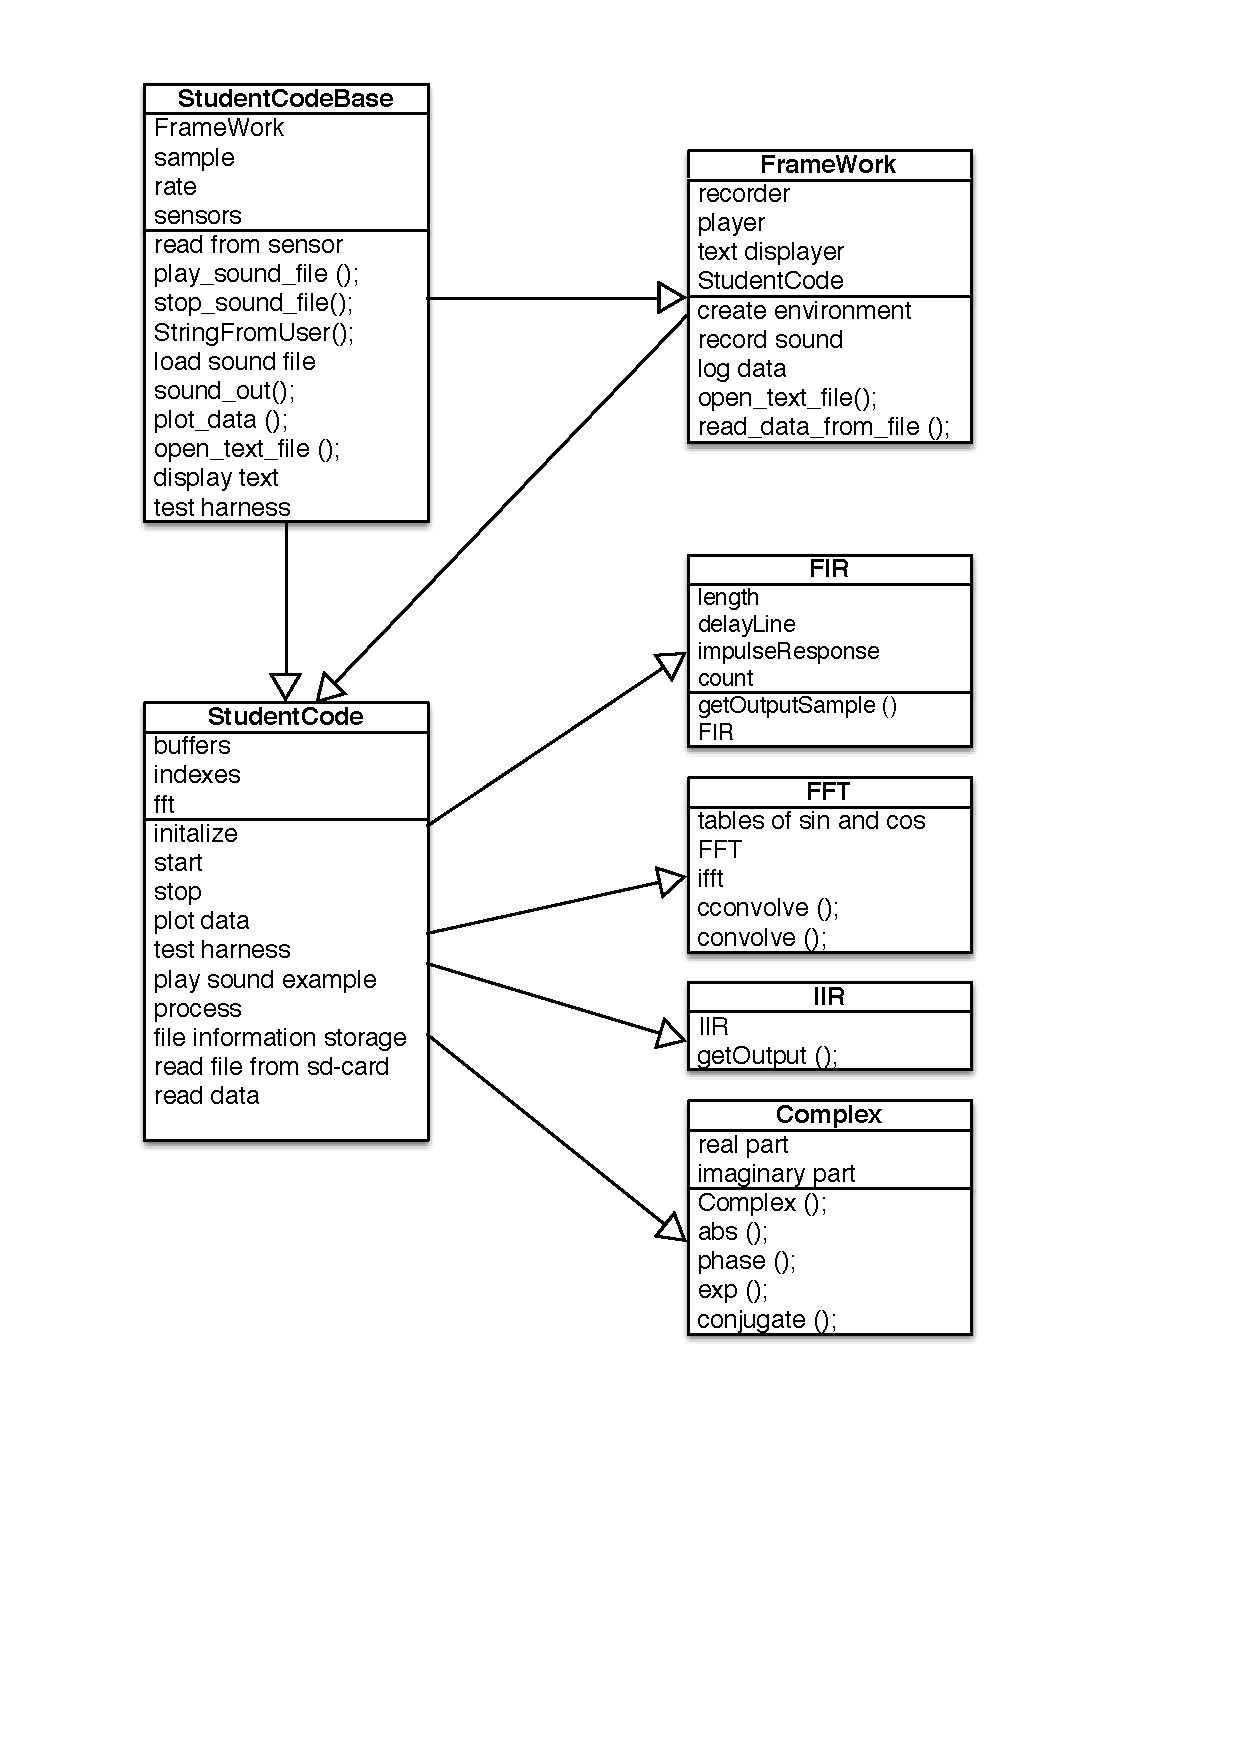
\includegraphics[width=0.6\textwidth]{UmlScheme.pdf}
    \caption[Description of FrameWork]{Description of FrameWork. }
    \label{fig:FrameWorkPicture}
\end{figure}



\section{App implementation} %Change the name for something else

Figure \ref{fig:SchematicsSystem} illustrates the schematic of our developed file transfer system. The user has the option to choose a file to be transmitted. After the file is selected the phone pulls the file from the SD-Card and encodes it into binary form. This binary stream is then modulated and sent through the channel. When the transmission is done the transmitting phone changes to an idle state while the receiving phone listens to the process and starts the demodulation after receiving the data. The file is reconstructed and stored on the receiving phone's SD-Card. The user now has the option to open the received file, otherwise the state of the receiving phone changes to idle.

 \begin{figure}[H]
  \centering
    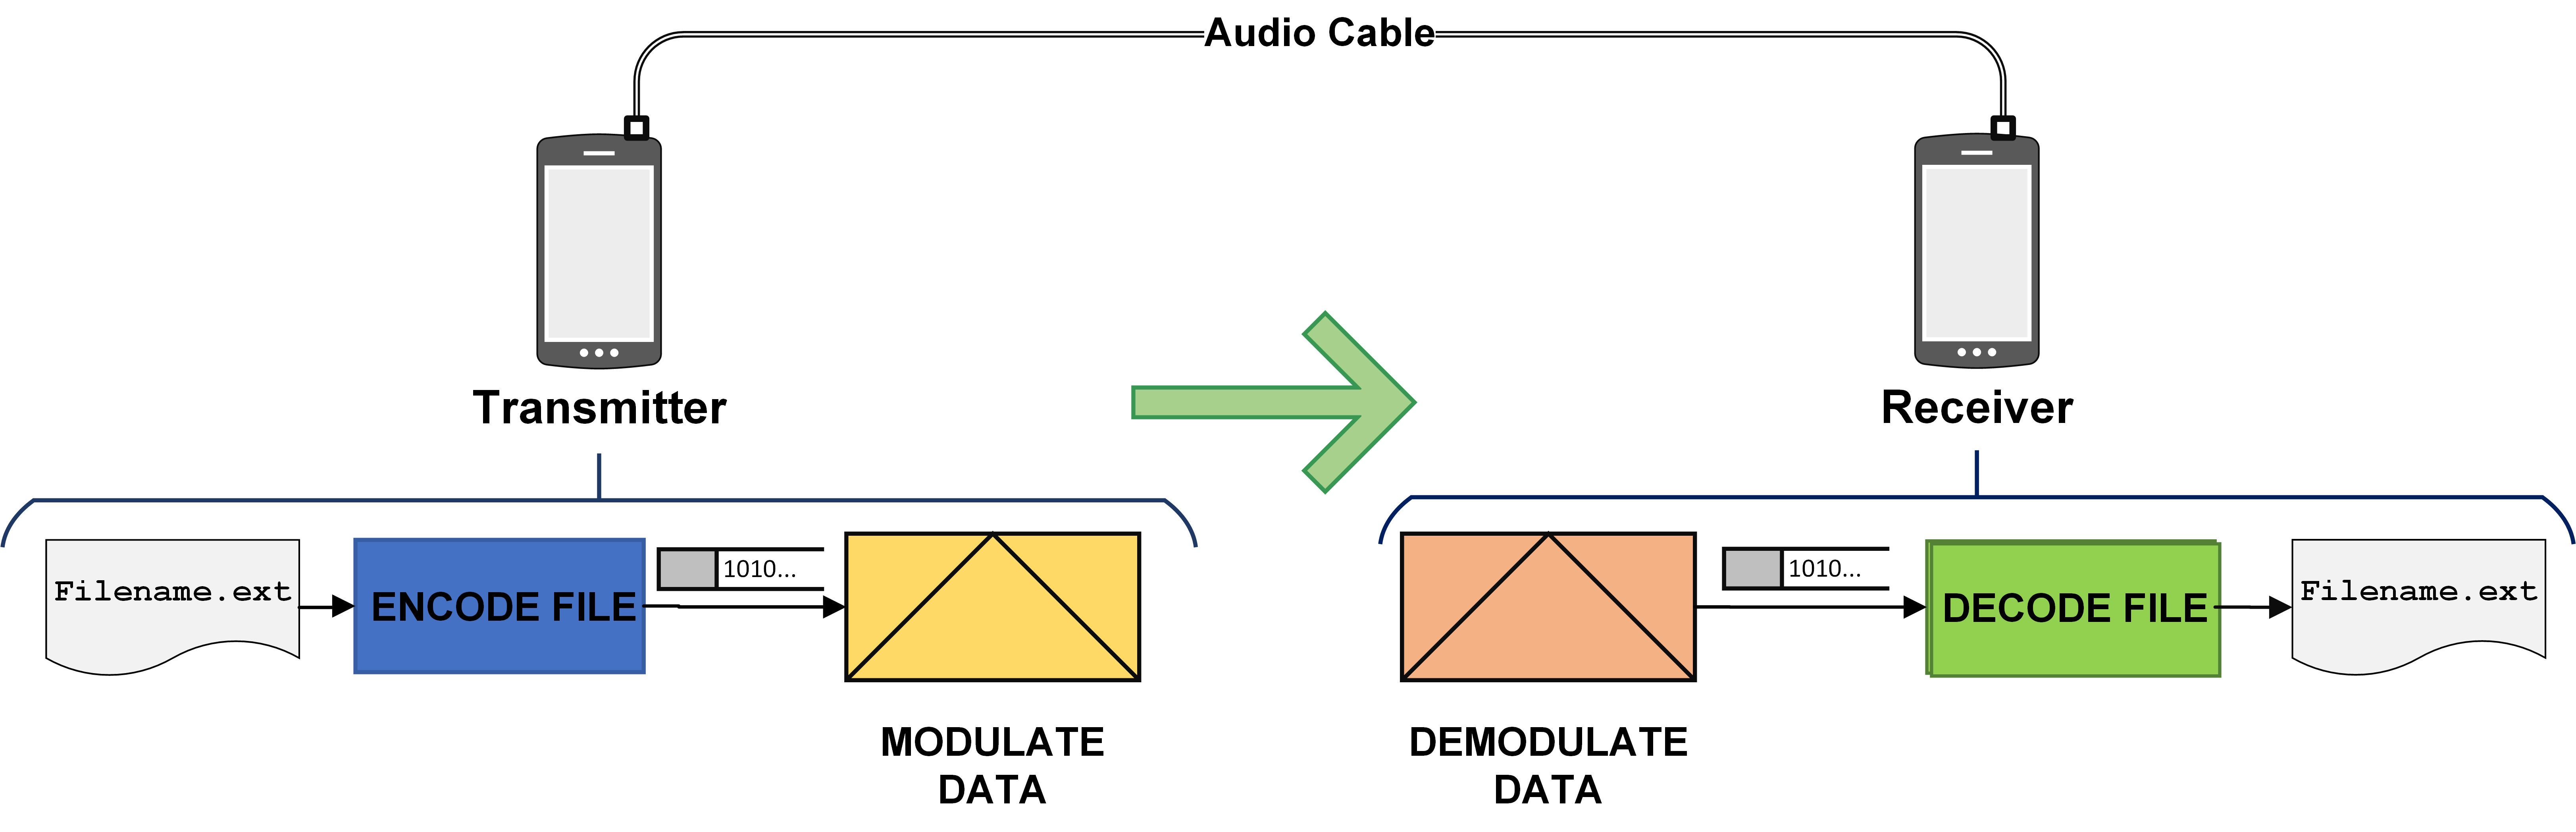
\includegraphics[width=1\textwidth]{FullSystem.png}
    \caption[Schematic of the file transfer system]{Schematic of the file transfer system.}
    \label{fig:SchematicsSystem}
\end{figure}


\clearpage
\subsection{Transmitter}

In figure \ref{fig:TXclient} a flow diagram of the transmitter functionalities are illustrated. The user chooses a file which is opened and read as an array of bytes. These bytes are then converted to a binary stream of ones and zeros, which are modulated with a given scheme along with a guard band and training sequence. The bits are then, modulated with a given scheme along with the guard-band and the training sequence. The total modulated signal (information data, guardband, training sequence and headers) is sent to the audio buffert, that plays the sound through the channel. The headers include the name, size and extension of the file along with a checksum value.

 \begin{figure}[H]
 \centering
 \begin{subfigure}[t]{.7\textwidth}
 \centering
    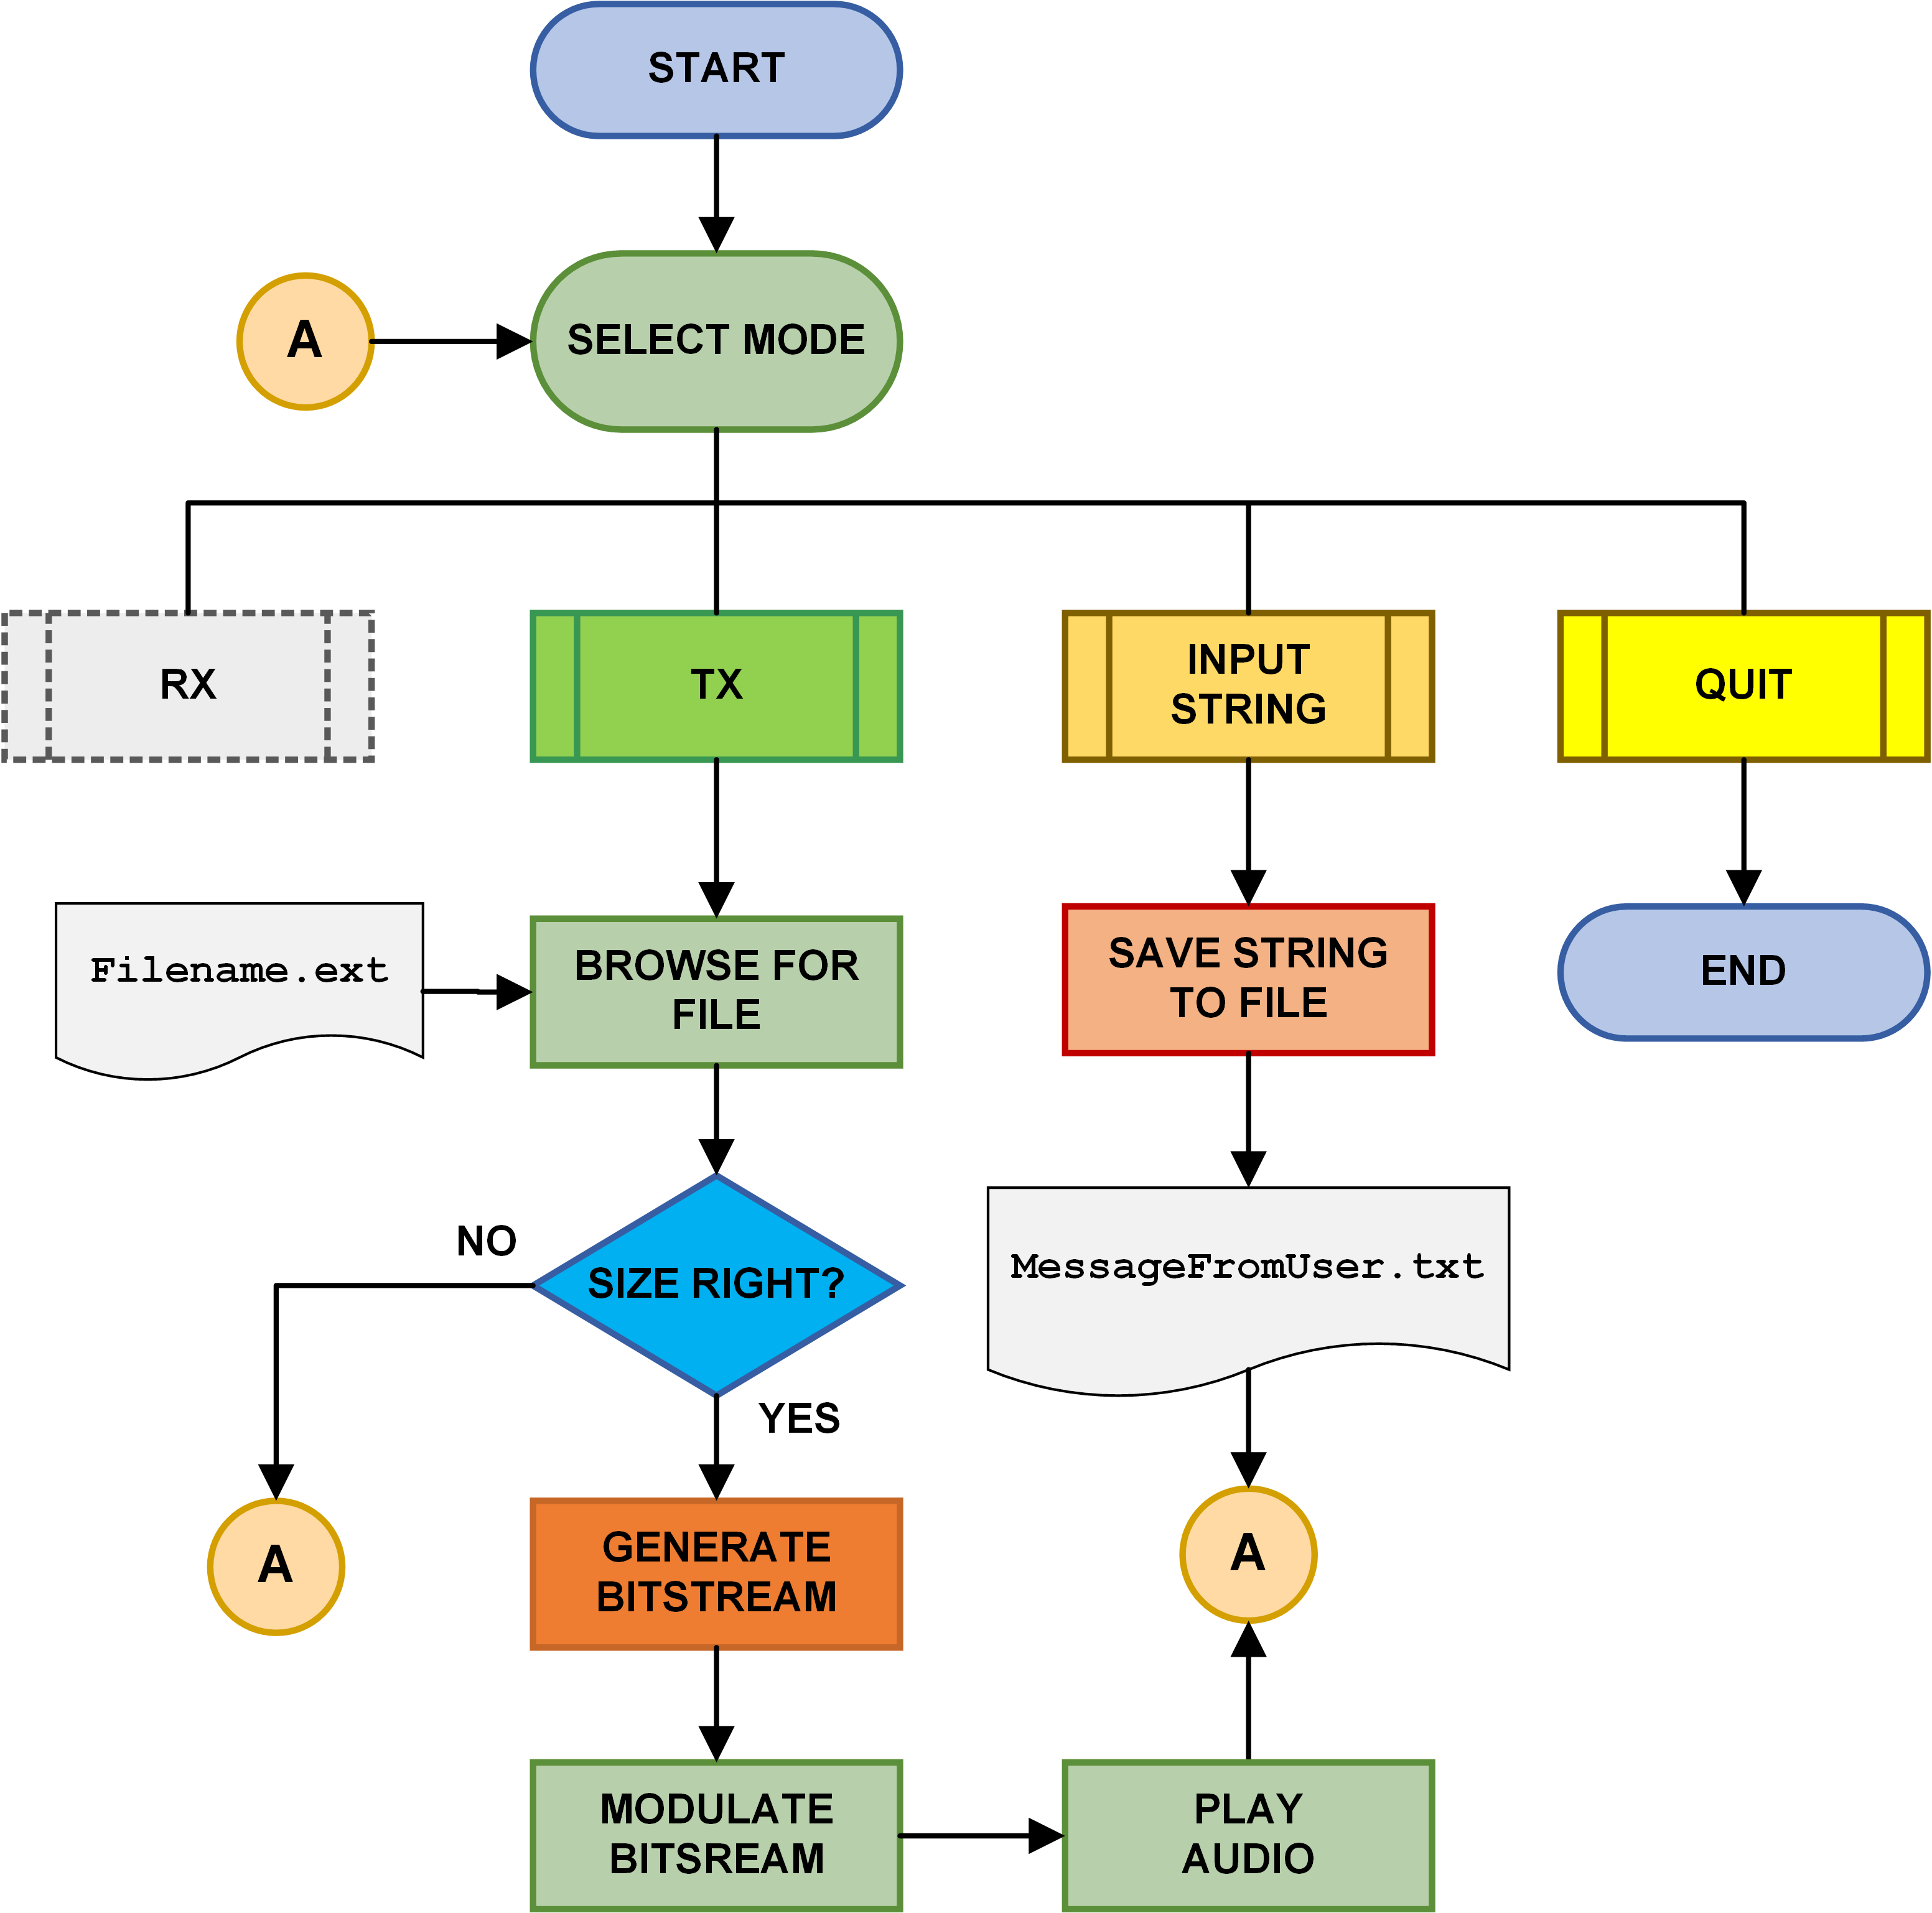
\includegraphics[width=0.8\textwidth]{TXschem.png}
    \subcaption{Full transmitter system.}
    \label{fig:TXclientFull}
    \end{subfigure}%
 \begin{subfigure}[t]{.3\textwidth}
  	 \centering
      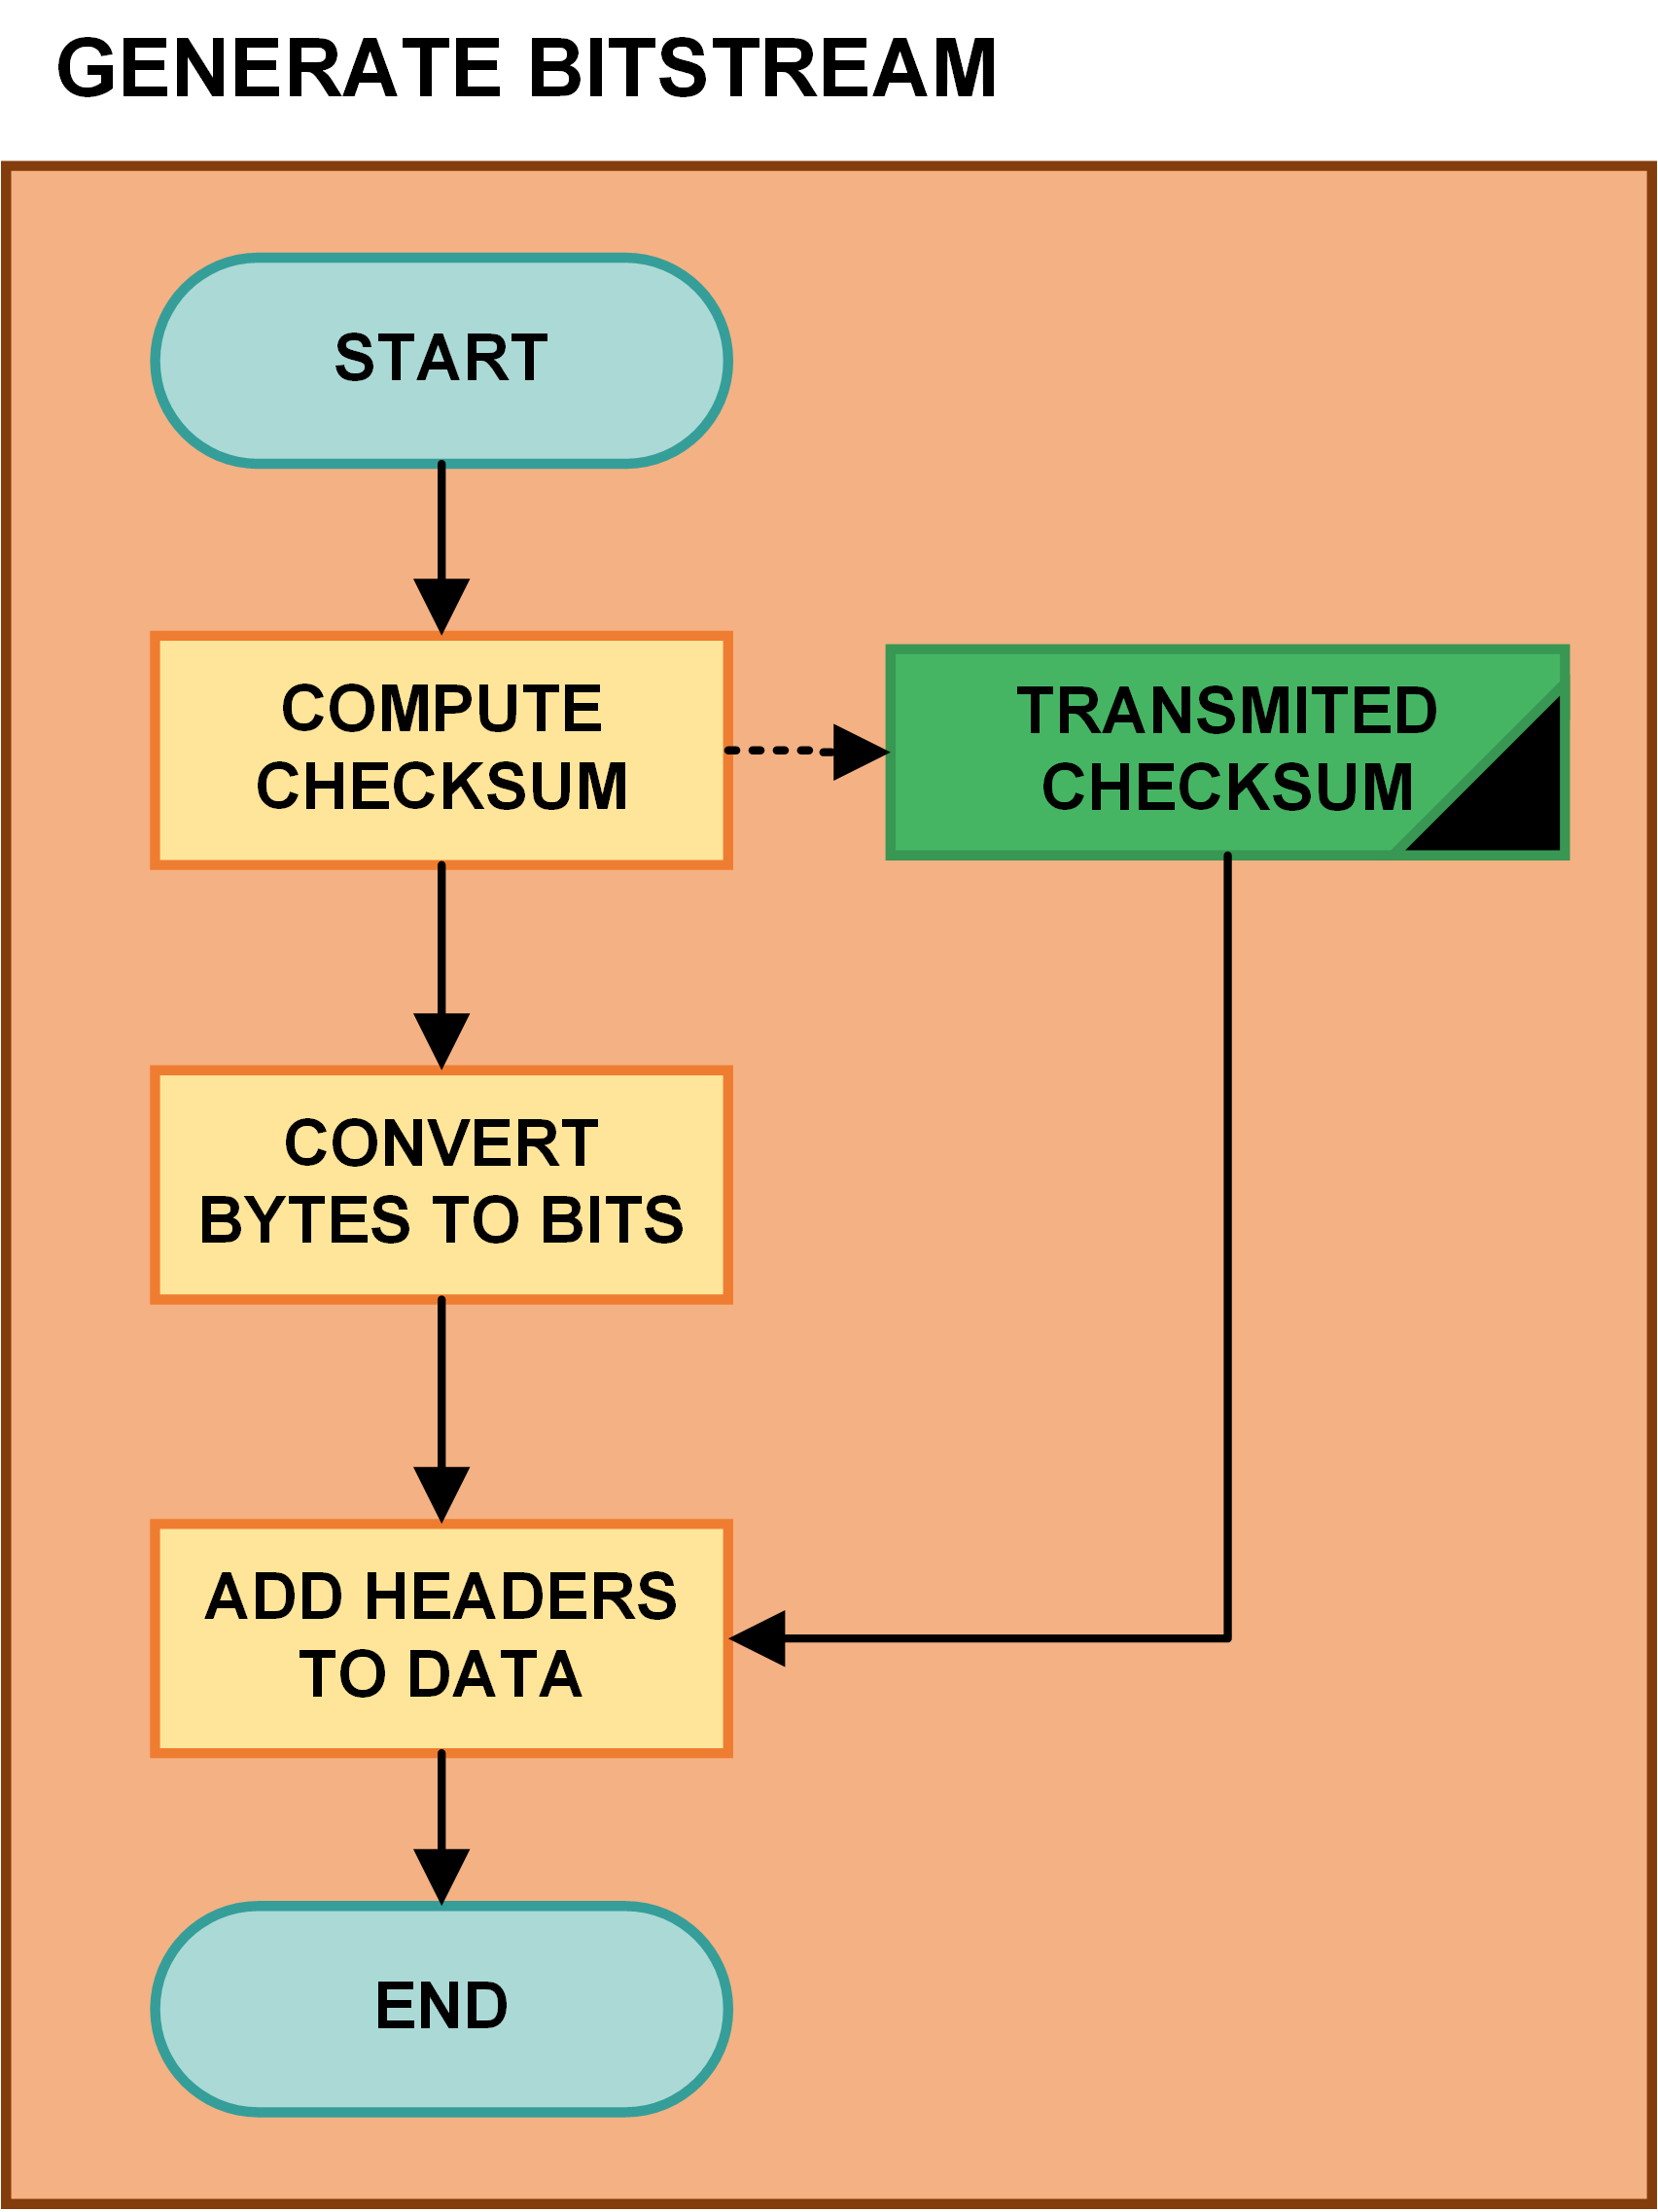
\includegraphics[width=0.8\textwidth]{schemGenBS.png}
      \subcaption{Generate Bit-stream diagram.}
      \label{fig:TXclientRecFile}
   \end{subfigure}
    \label{fig:TXclient}
    \caption[Transmitter client flow diagram]{Transmitter client flow diagram.}
 \end{figure} 

\subsection{Checksum}

The checksum used in our application is the internet checksum which is widely used in standard internet protocols. It takes a vector of bytes as input and performs the following operations:

\begin{itemize}
  \item Performs 1's complement sum of adjescent octets by combining them to one 16-bit integer
  \item Perform one last 1's complement on final checksum value \ldots
\end{itemize}

The checksum value is computed for our information data and is then sent through the channel. This value is retreived at the receiving phone, in order to make sure that the file is not corrupt during the transmission.


%\clearpage
\subsection{Receiver}

In figure \ref{fig:RXclient} a flow diagram of the receiver functionalities is illustrated, along with a diamgram of how the received file is reconstructed. The application starts listening if it varifies that there are samples above the detection threshold. If samples are below the threshold it is only noise otherwise the application starts buffering the input sound until the transmission is completed or the buffer is full. If the buffer is full, a new one is created. The received data is then processed and synchronized by correlating with a training sequence. Then the application applies the tone detection algorithm retrieving the binary stream of ones and zeros. The stream is processed and the name, size, data and checksum value of the selected file are retrived. The application uses this information to reconstruct the original file before saving it to the phones SD-Card. The user now has the option to either open the received file or return to the idle state.

 \begin{figure}[H]
 \centering
 \begin{subfigure}[t]{.7\textwidth}
 \centering
    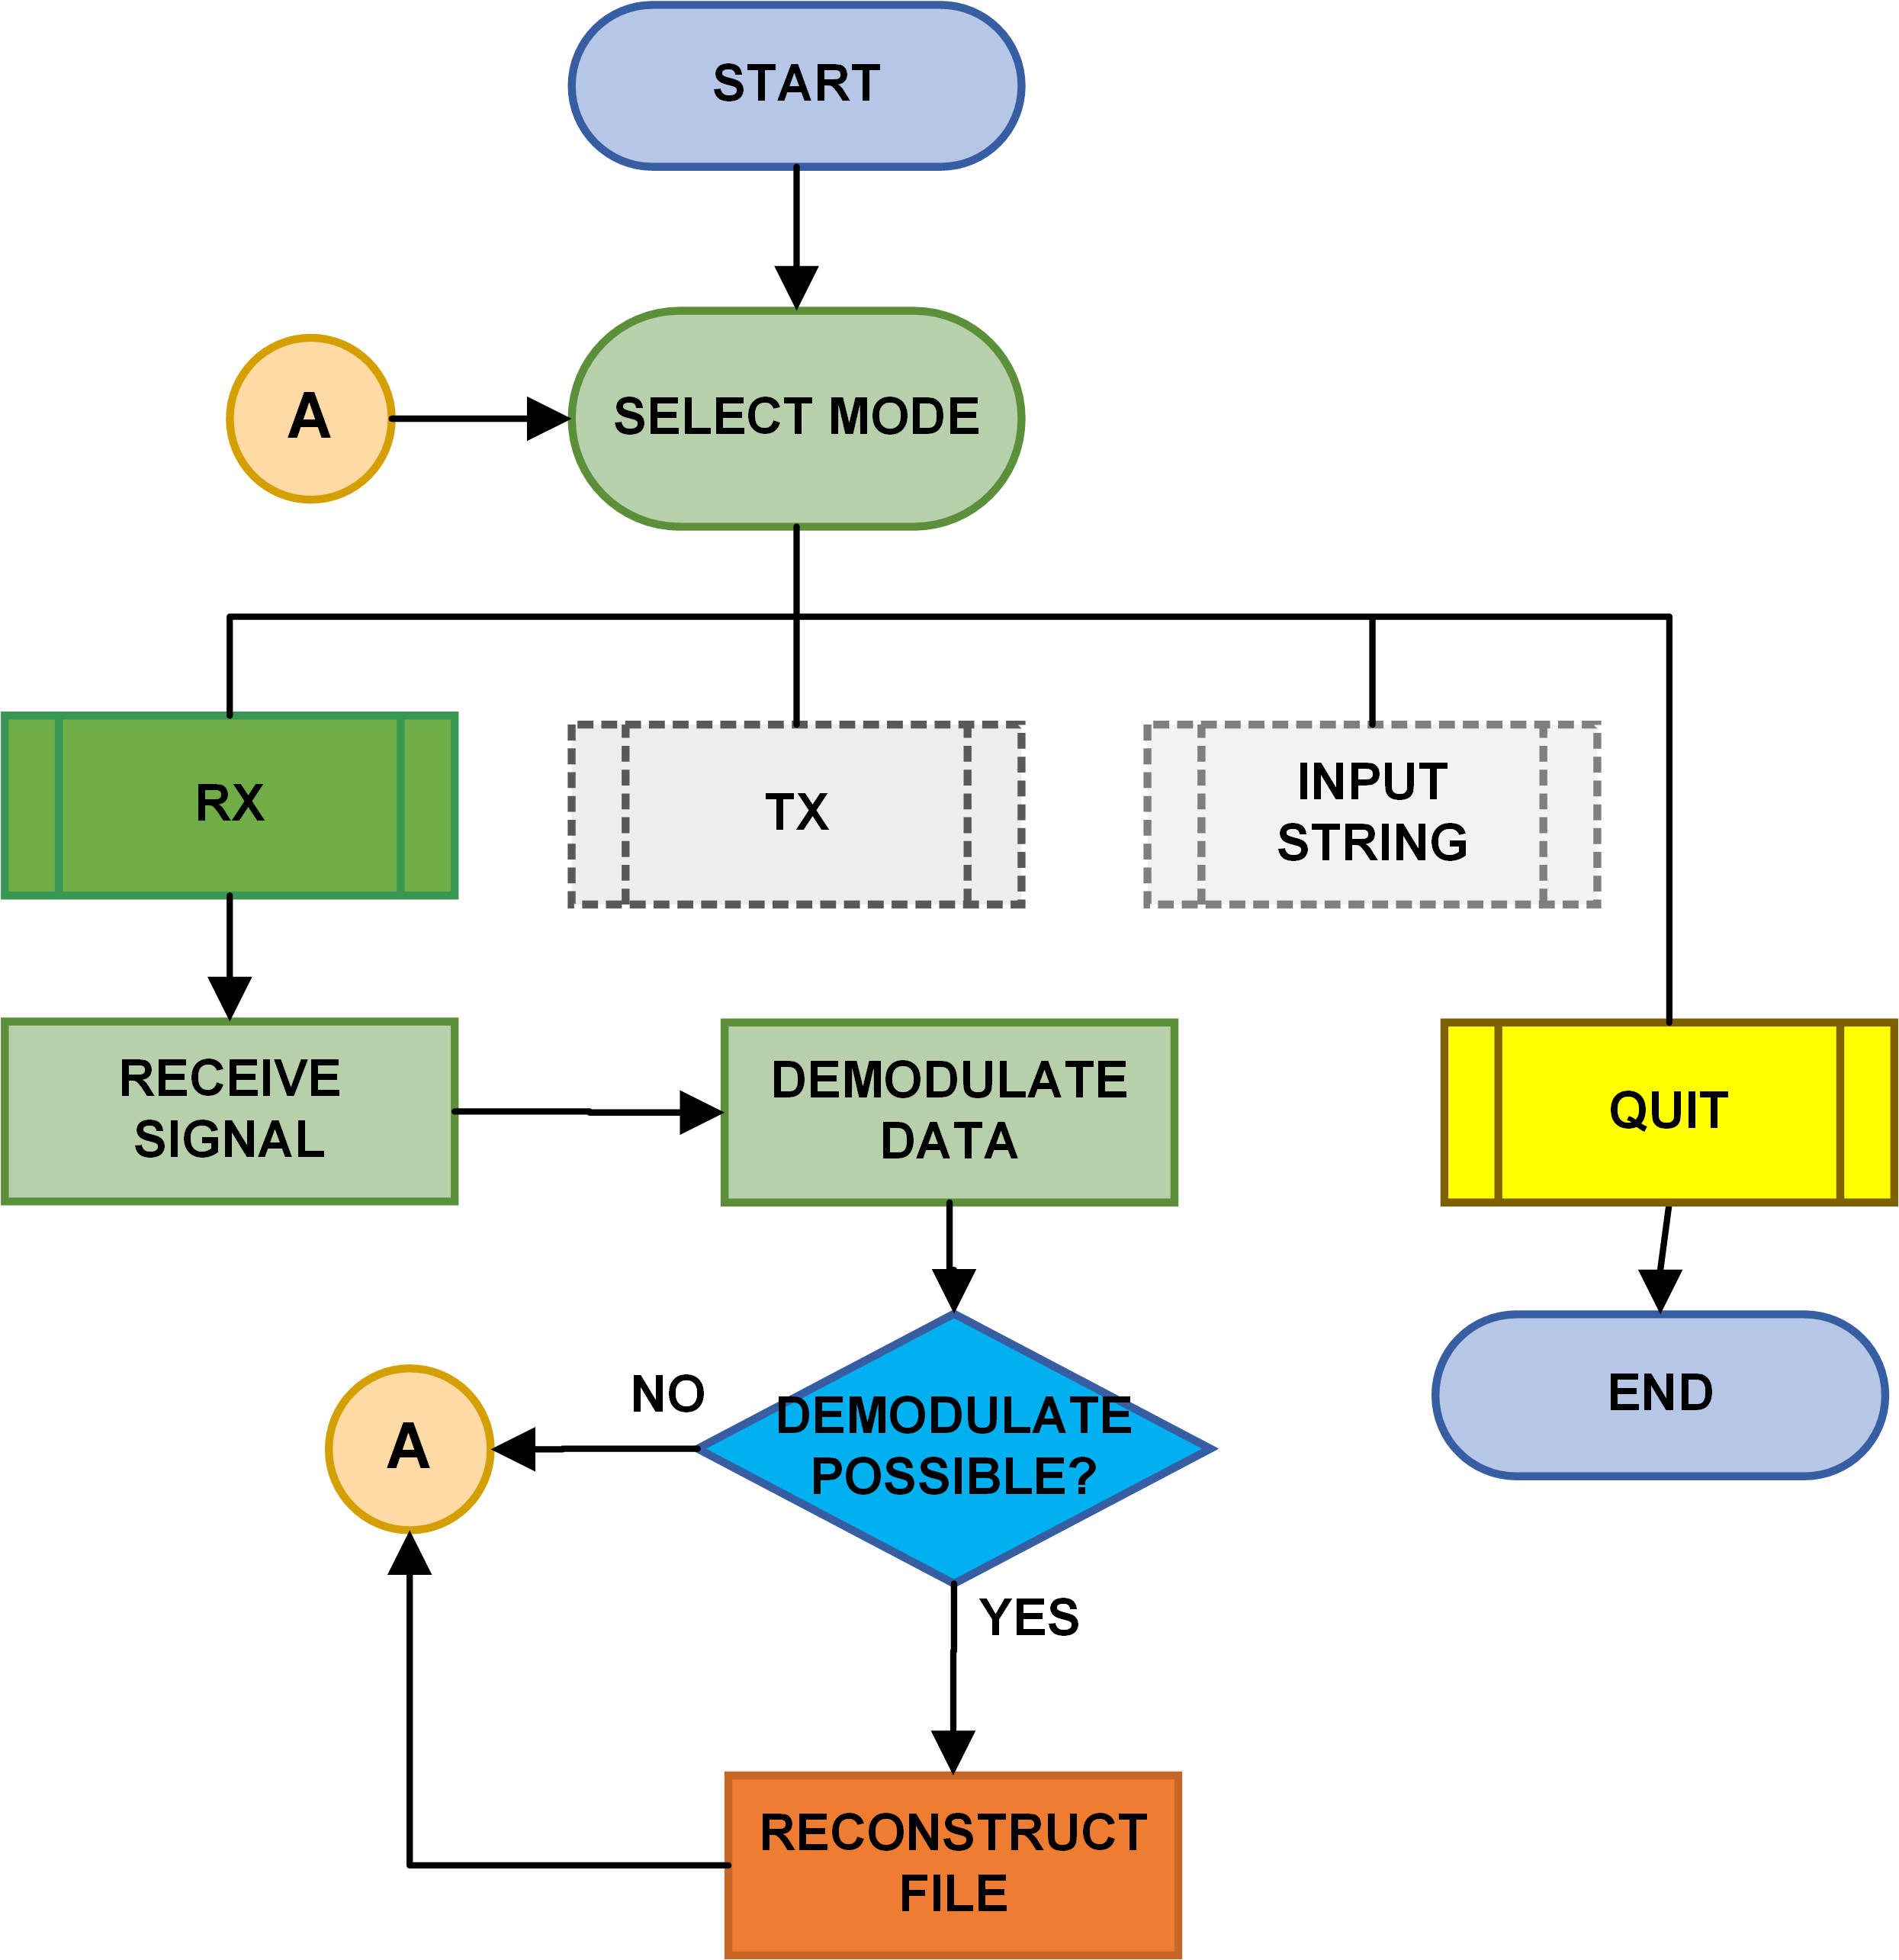
\includegraphics[width=0.8\textwidth]{RXschem.png}
    \subcaption{Full receiver system.}
    \label{fig:RXclientfull}
    \end{subfigure}%
 \begin{subfigure}[t]{.3\textwidth}
   \centering
      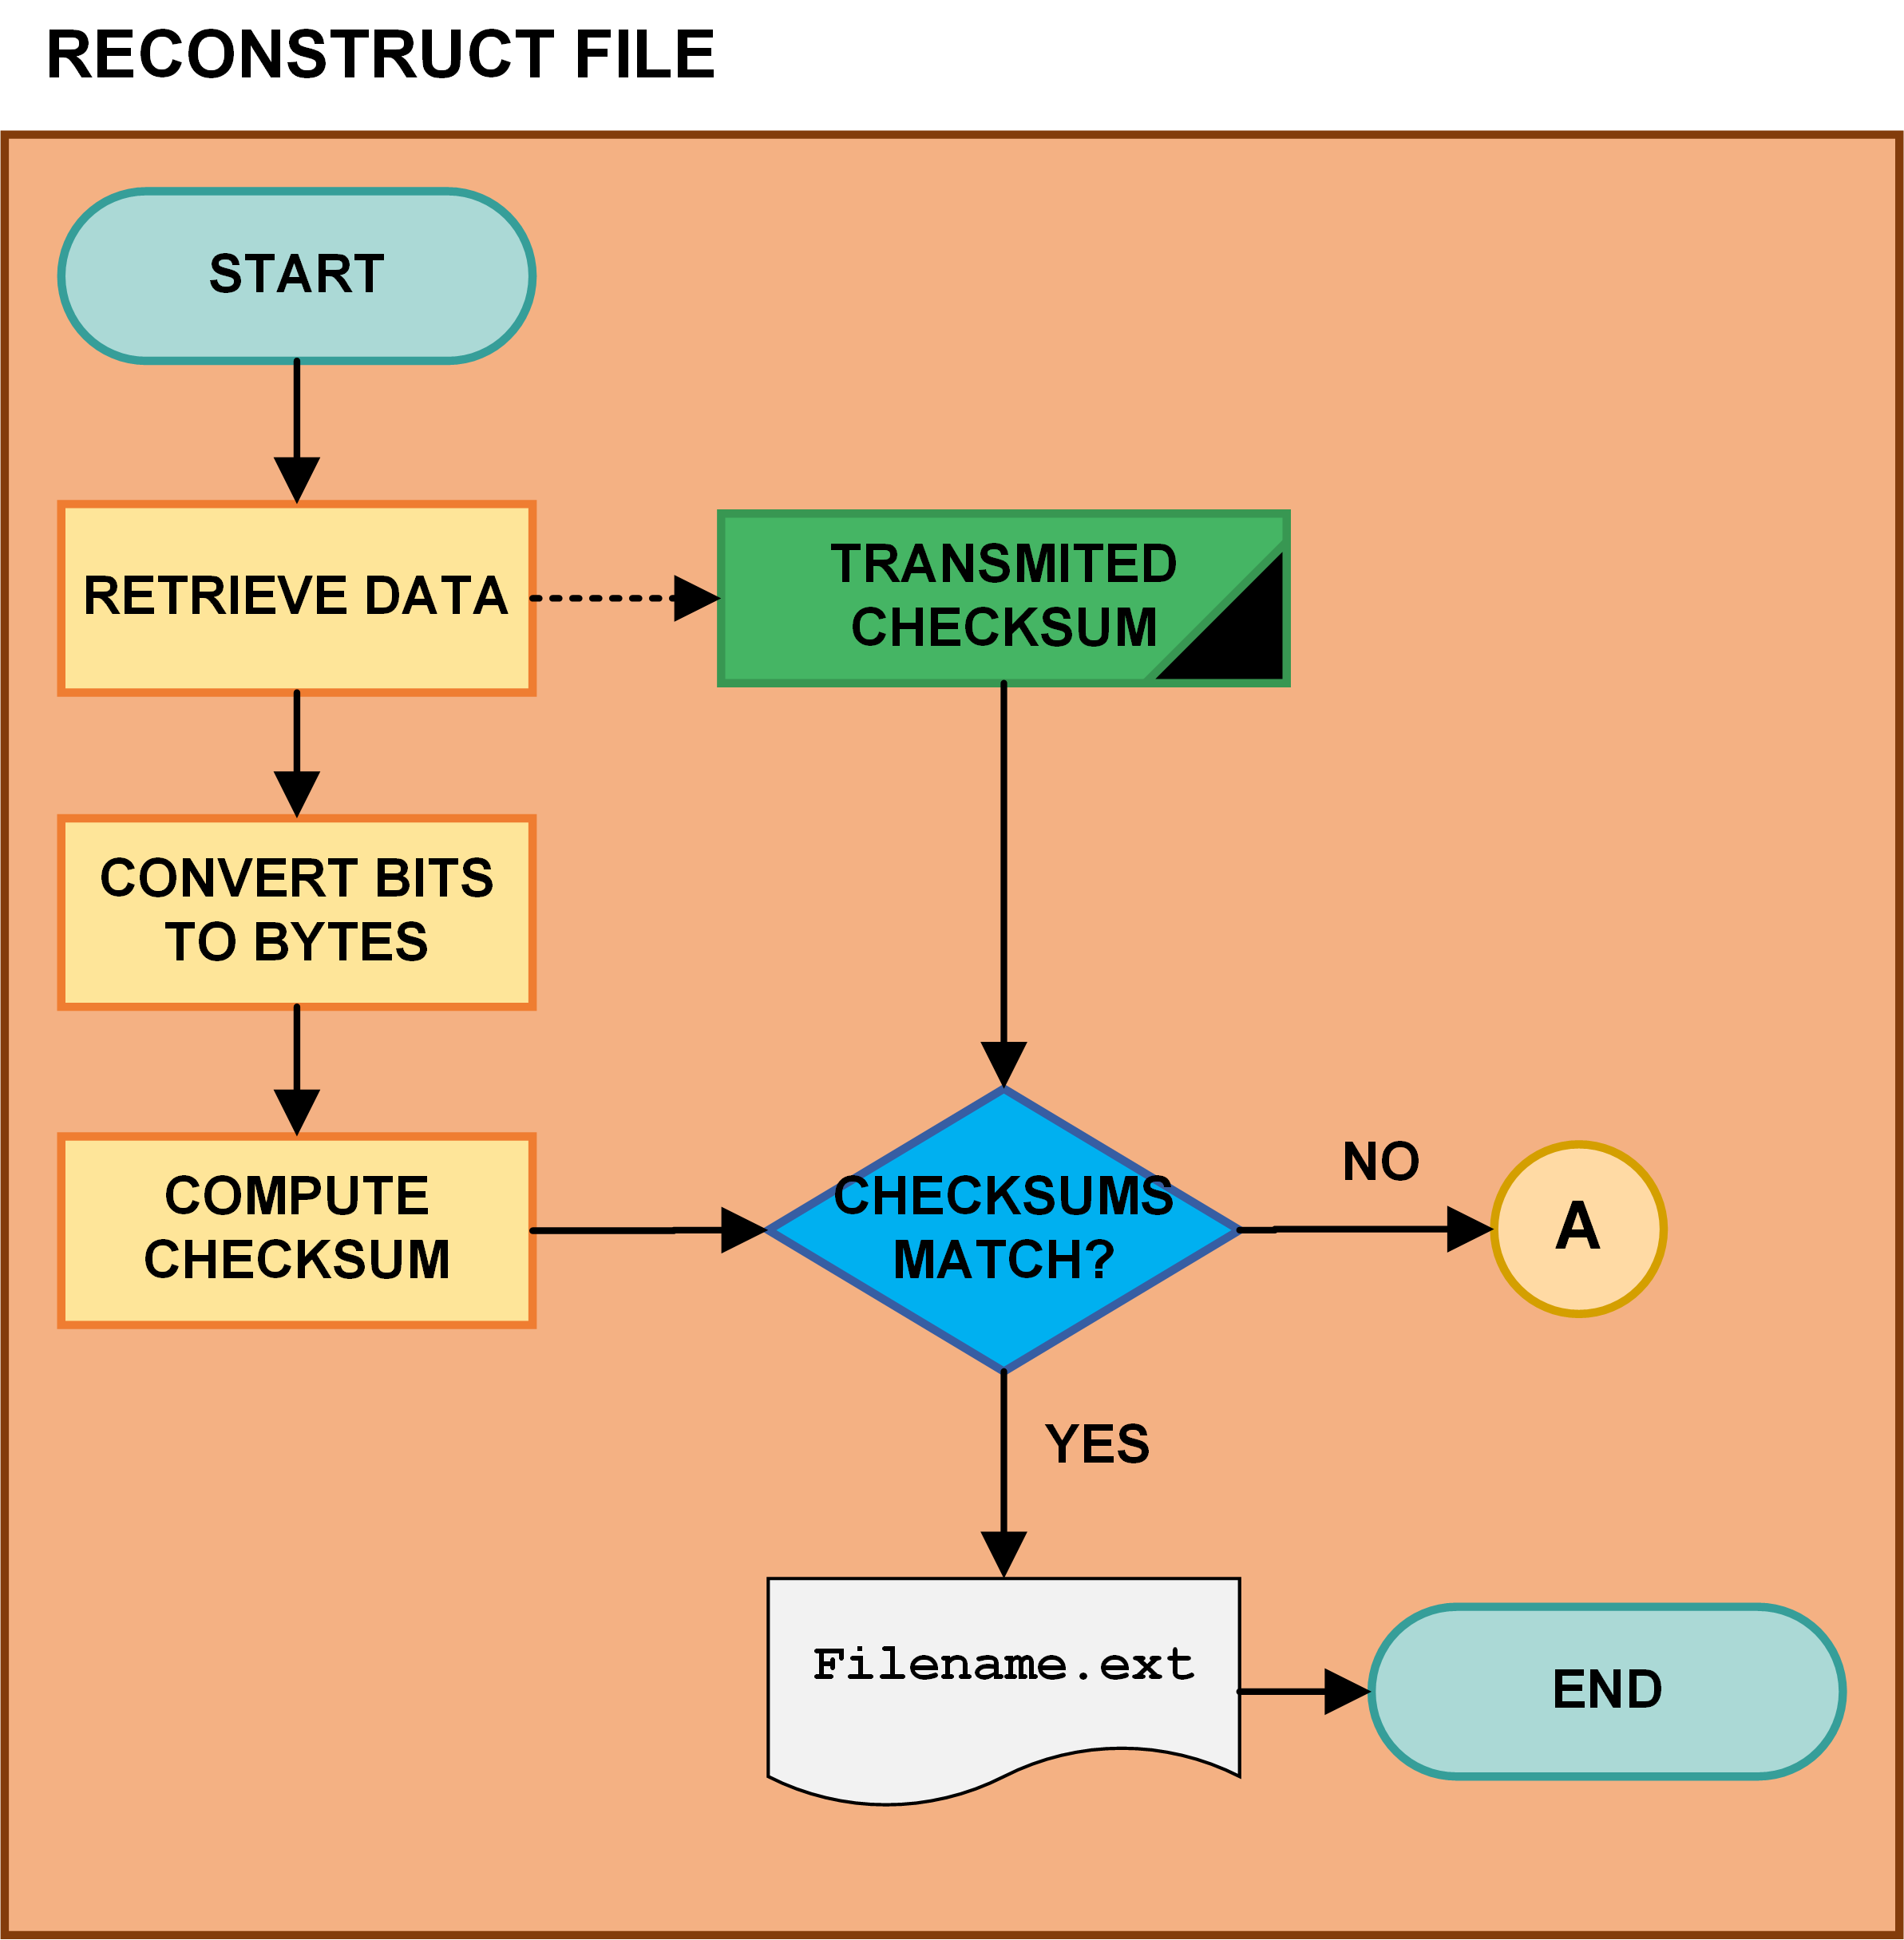
\includegraphics[width=1\textwidth]{RXreconstructSchem.png}
      \subcaption{Reconstruct file algorithm.}
      \label{fig:RXclientRecFile}
   \end{subfigure}
     \label{fig:RXclient}
      \caption[Receiver client flow diagram]{Receiver client flow diagram.}
 \end{figure} 

 
% % % % % % % % % % % % % % % % % % % % % % % % % % % % % % % % % % % % % % % % % % % % % % % % %
% % % % % % % % % % % % % % % % % % % % % % % % % % % % % % % % % % % % % % % % % % % % % % % %


\chapter{Method}

In chapter \ref{chap:Background}, the fundamentals of each modulation scheme were introduced. Now we will focus on developing the details and algorithms of our implementation in what refers to modulation, demodulation, channel adaptation and coding techniques. 

\section{M-FSK system}

Our first design consists in a system based on FSK modulation with off-line and real-time implementations. The used system is a M-ary FSK system (2-FSK for syncronization and 4-FSK for data modulation) with orthogonal envelopes to improve the BW efficiency of the MFSK modulation. 

\subsection{M-FSK transmiter}

With a 4 FSK system, it is possible to transmit $\log_2(4)=2$ bits per symbol. It is then necessary to compute the frequencies that will accommodate the transmitted symbols. Denote $n_{sym}$ as the number of samples per symbol. In order to increase the efficiency for our decoding scheme, the frequencies should be chosen such that:
\begin{equation}
f_k=f_s \times \frac{k}{n_{sym}}
\end{equation}

These are the bins-center frequencies and they should have a sufficiently large minimum distance between them so that the peaks do not become indistinguishable. This requirement is of particular importance since the demodulation method is based in a DFT-based algorithm that will be described in section \ref{sec:FSKdemod}. %it would be nice to have 2 plots, one where the frequencies are very close and another where the frequencies are very spread%
Once the frequencies are picked, the transmitter merges the bits to be transmitted with the ones from the training sequence and guard bands and modulates them accordingly. The samples that correspond to the \emph{n-th} symbol are given by:
\begin{equation}
s(k) = \cos{(2\pi \frac{ f_i}{f_s} k)}, \ k=n\times n_{sym} +1, ... , n \times n_{sym}+n_{sym}
\end{equation}
Where $f_i$ is the frequency that matches with the symbol that is to be transmitted.
 
 
  
\subsection{M-FSK receiver}
In the receiver side, the first step is to synchronise and find the beginning of the training sequence. When the receiver knows where the transmission starts, the samples are then input for the decoding algorithm. 

The demodulators presented in part \ref{subsec:fsk} are interesting from a theory point of view. However, for real time, software-based applications there are other methods for efficient demodulation. One of these methods is the Discrete Fourier Transform (DFT) which evaluates the amplitude and phase for each frequency present in the received signal. Since we are using a M-FSK modulation scheme, a tone/frequency detector such as the DFT for a symbol period is a powerful tool for a correct and efficient demodulation. However, we are only interested in detecting one or more tones in an audio signal and at the same time we are constrained to the CPU horsepower provided by the smartphone. Taking this into account, we purpose a much faster method, when compared with FFT for instance, which is the Goertzel algorithm. 


\subsubsection{Goertzel Algorithm}
\label{sec:FSKdemod}

There are various ways to detect the presence of a special known frequency in a received signal. The DFT algorithm is a simplistic way to check whether the desired frequency is present and a FFT produces the same numerical result for a single frequency of interest, making it a better choice for tone detection. The Goertzel algorithm is a DFT in disguise, with some numerical tricks to eliminate complex number arithmetic, increasing the efficiency over the FFT under some constraints.

The idea is to transform an ordinary N samples DFT into a Goertzel filter form. Defining $W_N^{k}={e^{ - j2\pi k/N}}$, and noting that $W_N^{^{ - Nk}} = 1$, we have for the DFT \cite{GoertzelPaper}:
\begin{equation}
X(k) = \sum\limits_{n = 0}^{N - 1} {x(n)W_N^{nk}}  = \sum\limits_{n = 0}^{N - 1} {x(n)W_N^{ - Nk} \cdot W_N^{nk}}  = \sum\limits_{n = 0}^{N - 1} {x(n) \cdot W_N^{^{ - (N - n)k}}} 
\end{equation}

An efficient way to evaluate this polynomial is the nested form:
\begin{equation}
X(k) = \left\{ {\left[ {\left( {W_N^{ - k}x(0) + x(1)} \right)W_N^{ - k} + x(2)} \right]W_N^{ - k} +  \cdots  + x(N - 1)} \right\}W_N^{ - k}
\end{equation}

The last expression can be written in terms of a recursive difference equation:
\begin{equation}
y(n) = {W^{ - k}_N}\cdot y(n - 1) + x(n)
\end{equation}
\[
\]

Expressing the difference equation in the z-transform domain and by multiplying both numerator and denominator by (${1 - {W_N}^{ - k}{z^{ - 1}}}$), we get the transfer function:

\begin{equation}
\frac{{Y(z)}}{{X(z)}} = H(z) = \frac{1}{{1 - {W_N^{ - k}}{z^{ - 1}}}} = \frac{{1 - W_N^{ - k}{z^{ - 1}}}}{{1 - (2\cos (\frac{{2\pi k}}{N}){z^{ - 1}} - {z^{ - 2}})}}
\end{equation}

The Goertzel algorithm acts as an IIR filter that uses the feedback path to generate a very high $Q$ bandpass filter, where the coefficients are easily generated from the required center frequency.  \textcolor{red}{It is mostly implemented as the second order recursive IIR filter}, as shown in figure \ref{fig:IIR}. 
%Rewrite the sentence

 \begin{figure}[H]
  \centering
    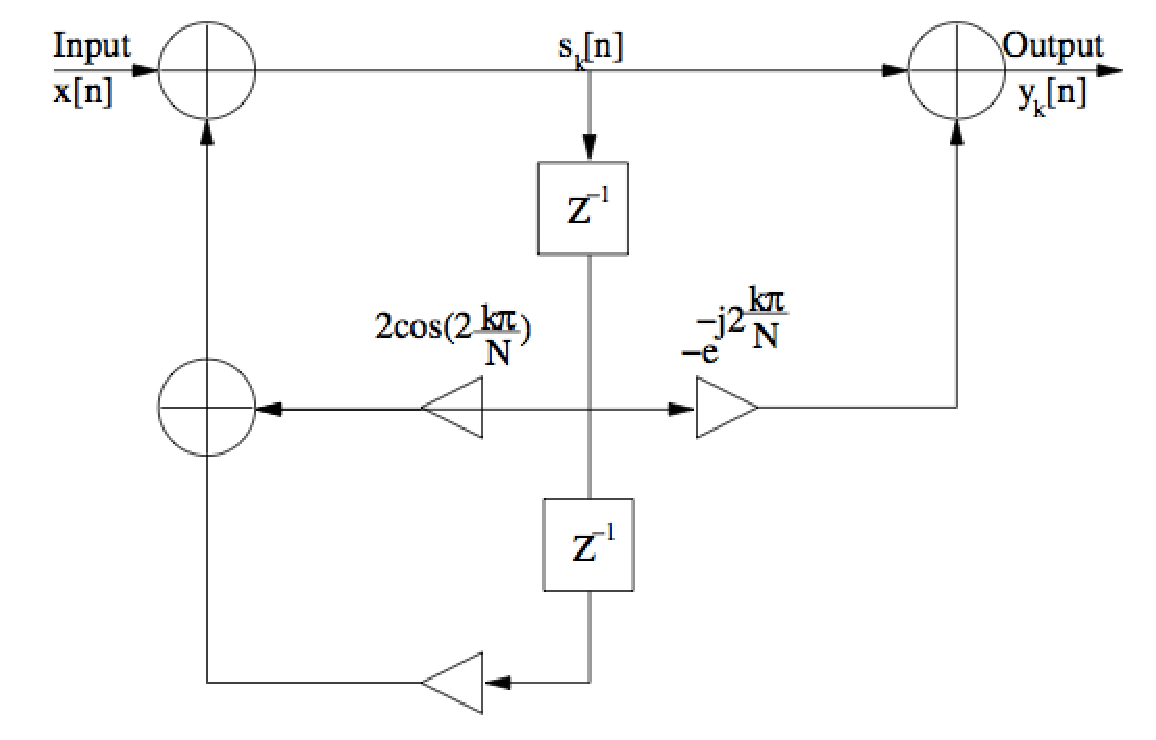
\includegraphics[width=0.5\textwidth]{IIR.pdf}
    \caption[Direct-Form realisation of the Goertzel algorithm]{Direct-Form Realisation of the Goertzel Algorithm \protect\cite{HaykinBook}.}
    \label{fig:IIR}
\end{figure}


The algorithm computes the k-th DFT coefficient $X(k)=y(N)$ of the input signal $x(n)$ using the 2nd order filter:
\begin{equation}
\begin{array}{lll}
{y_k}(n) & = & {s_k}(n) - W_N^k{s_k}(n - 1),\\
\text{with } & &{s_k}(n) = x(n) + 2\cos (\frac{{2k\pi }}{N}){s_k}(n - 1) - {s_k}(n - 2),\\
\text{and } & & {s_k}( - 1) = {s_k}( - 2) = 0

\end{array}
\label{fig:IIRtime}
\end{equation}

The discrete frequencies in which the algorithm is able to compute the DFT are ${f_k} = \frac{k}{N}{f_s}$, for $f \leq \frac{f_s}{2}$.
%%The computation for $s_k(n)$ takes one add ($x(n)-s_k(n-1)$) and one %%multiply-accumulate per received sample.

\subsubsection{Computational and Memory complexities}

The FFT algorithm used with $N$ being a power of two has computational demands proportional to $\mathcal{O}(N\log_2 N)$. The absolute number depends on the particular implementation. Usually, the number of real-number arithmetic operations found in the literature is approximately $6N \log_2 N$. If we analyse the number of operations of the Goertzel algorithm, we realize that for a real input signal, $N$ real multiplications and $2N$ real additions are performed and, hence, $3N$ operations for a single frequency are required. Ignoring the computations of the cosine and the exponential constants in equation \ref{fig:IIRtime}, and for $N$ frequencies, we have that the Goertzel algorithm has quadratic complexity like the DFT. To clarify for how many frequencies ($K$), it is perfered to use the Goertzel algorithm insted of FFT \cite{GoertzelPaper}, one can compare the complexity of both and conclude that: 


\begin{equation}
3NK < 6N{\log _2}N \Leftrightarrow K < 2{\log _2}N
\label{eq:ineffgor}
\end{equation}

Such  result holds only for $N$ being a power of two; otherwise the inequality \ref{eq:ineffgor} can even be more favourable for the Goertzel algorithm.

Considering real inputs solely, the FFT algorithm requires a memory space of at least $2N$ samples. Also, the $n$ values of the transformation kernel, $sin$ and $cos$, are often precomputed and stored. The FFT calculation itself can be performed with no values being moved in memory, but as the computation cannot be done until the last sample of a block of data is received, a buffer size of at least $N$ samples must be used. Therefore, the overall FFT memory demand is $4N$ for real signals.
For each considered frequency, the Goertzel algorithm requires: location for saving one real and one complex state variable, the complex final output and the last 2 real outputs $s_k(n)$ and $s_k(n-1)$. There is no need to implement input buffering, because the computation can be run as the new signal samples arrive. The total memory complexity of the Goertzel algorithm is, thus $7K$ positions. Combining all the above together, the Goertzel algorithm will be less memory-demanding than the FFT if \cite{GoertzelPaper}
\begin{equation}
7K < 4N \Leftrightarrow K < \frac{4}{7}N
\end{equation}


As long as $N\geq 13$, equation \ref{eq:ineffgor} is decisive for choosing the best algorithm, since for these $N$ it holds that $\frac{4}{7} N \leq 2 \log_2 N$.

\subsubsection{Pseudo-code for decoding algorithm}
The pseudo-code of the implemented algorithm for the index $k$ of the DFT spectral component is as stated in algorithm \ref{goeralg}:  \\

\begin{algorithm}[H]
\SetKwData{Left}{left}\SetKwData{This}{this}\SetKwData{Up}{up}
\SetKwFunction{Union}{Union}\SetKwFunction{FindCompress}{FindCompress}
\SetKwInOut{Input}{input}\SetKwInOut{Output}{output}
\Input{index $k$ of the DFT spectral component; signal $x$ of length $n_{sym}$}
\Output{y, representing $X[k]$}
\BlankLine
\emph{\% Precalculation of constants}\;
$A= 2\pi \frac{k}{N}$\;
$B = 2\cos{A}$\;
$C = \exp{(-jA)}$\;
\emph{\% State variables}\;
$s_0=0$\;
$s_1=0$\;
$s_2=0$\;

\emph{\% Main loop}\;
\For{{$i=0$ : $N-1$}}{  \emph{\% N multiplications, 2N additions}\;
$s_0 = x[i] + B\times s_1 - s_2$\;
$s_2 = s_1$\;
$s_1 = s_0$\;
}

\emph{\% Finalizing calculations}\;
$s_0 = B\times s_1 - s_2; $ \emph{\% 1 multiplication and 1 addition}\;
$y = s_0 -s_1 \times C; $  \emph{\% 4 multiplications and 3 additions}\;
\BlankLine
\BlankLine
\caption{Goertzel Algorithm to estimate the $k$:th spectral component of signal $x$ of length $N$.}
\label{goeralg}
\end{algorithm}


After demodulation, the decisions are sent to the decoder and the BER is computed. Denoting $n_{sym}$ as the number of samples per period, the rate for a 4-FSK system is given by:
\begin{equation}
R = \frac{log_2(4)}{n_{sym}}\times f_s = \frac{2}{n_{sym}}\times f_s 
\end{equation}

\textcolor{red}{ADD: A general description of the used transmitter, pseudo-code, and major functions. IF NECESSARY}%
\clearpage


\section{M-QAM system}
In order to meet the data throughput requirement, we considered to use a configurable M-QAM scheme to achieve the highest possible rate without compromising the performance and still with zero or a negligible amount of errors that could be corrected. In the case of the real-time implementation, we use a checksum comprobation to confirm the data integrity instead of FEC, however for the case of off-line test, we tried with different coding schemes. The results of such test are described in section \ref{sec:ChanCodTests}.
%Work on this

\subsection{M-QAM transmitter}
	There are a considerable set of parameters in the transmitter that will determine the performance of the system. We enlist the most important next:



\begin{description}{\bfseries}
  \item[\bf{$N_b$}]; number of bits to be transmitted.
  \item[\bf{$f_s$}];  sampling rate. The maximum value accepted by the phones is 44.1 kHz.
  \item[\bf{Window}]; discrete window coefficients. Each window has different parameters which will influence the impulse and frequency responses (such as the roll-off factor in the RRC or the $\alpha$ in Gaussian window).
\item[\bf{$n_{sym}$}]; number of samples per symbol. 
  \item[\bf{$levels$}]; order of the constellation. 
\item[\bf{$f_c$}]; carrier frequency. 
\end{description}


The sampling frequency, the number of samples per period and the order of the constellation will determine the rate of the system according to:
\begin{equation}
R = \frac{{2 \times levels}}{{n_{sym}}} \times f_s
\end{equation}


After these parameters are set, the algorithm comes into action. The first step is to merge the bits in the following order:
\[
[\textbf{guard\_band   $\mid$  training seq.  $\mid$   bit\_stream  $\mid$   guard\_band}]
\]

Subsequently, the bits are mapped into the constellation (MQAM) according to the pseudo-code in algorithm \ref{mod}. 


\begin{algorithm}[H]
\SetKwData{Left}{left}\SetKwData{This}{this}\SetKwData{Up}{up}
\SetKwFunction{Union}{Union}\SetKwFunction{FindCompress}{FindCompress}
\SetKwInOut{Input}{input}\SetKwInOut{Output}{output}
\Input{bit stream; \%data to be transmitted}
\Output{z; \%Complex modulated symbols $z = x + jy$}
\BlankLine
\emph{\%Initialization of vectors}\;
mx=[]\;
my=[]\;

\For{{$n=first symbol$ \KwTo $last symbol$}}{
\emph{\%Initialize values of $x_i$ and $y_i$}\;
$x_i$=0\;
$y_i$=0\;
\emph{\%Pick 2 bits of the symbol at each time}\;
\For{{$m=first bit $ : 2 :  $last bit$}}{
\eIf{bit stream(n+m)==0}
{$xi = xi + 2 ^\frac{{m-1}}{2}$\;
}{$xi = xi - 2 ^\frac{{m-1}}{2}$}

\eIf{bit stream(n+m+1)==0}
{$yi = yi + 2 ^\frac{{m-1}}{2}$\;
}{$yi = yi - 2 ^\frac{{m-1}}{2}$}
}
mx=[mx xi]\;
my=[my yi]\;
}
z = mx + $j$my
\caption{Modulation of MQAM symbols.}
\label{mod}
\end{algorithm}

 The discrete carriers to modulate the signal are then generated and have $n_{sym}$ samples:
\begin{equation}
\left\{ \begin{array}{l}
\cos (2\pi f_ck)\\
 - sin(2\pi f_ck)
\end{array} \right.\text{, with }  k = 0,\frac{1}{{f_s}},\cdots,\frac{{n_{sym}}}{{f_s}} - \frac{1}{{f_s}}
\label{eq:MQAMdiscCarriers}
\end{equation}

The window is also generated in the initialization of the program:
\begin{equation}\label{eq:window}
W_{n_{sym}}(i) = w_i\text{ , with }i = 1,2,\cdots,n_{sym}
\end{equation}

 The coefficients $w_i$ in \ref{eq:window} are computed according to the previously chosen window. Then, the complex symbols, the window and the carriers are mixed together to generate the discrete transmitted waveform. The generated samples for the $\emph{n-th}$ symbol have the following expression:

\begin{equation}\begin{array}{l}
s(k) = \Re (z) \cdot {W_{{n_{sym}}}}(k\% {n_{sym}}) \cdot \cos (2\pi \frac{{{f_c}}}{{{f_s}}}k) - \Im (z) \cdot {W_{{n_{sym}}}}(k\% {n_{sym}}) \cdot \sin (2\pi \frac{{{f_c}}}{{{f_s}}}k)\\
\text{with $k = n \cdot n_{sym} + 1,\cdots,n \cdot n_{sym}+ n_{sym}$ ; and with \% as the modulo operator.} 
\end{array}\end{equation}

The signal $s(k)$ is then normalized to be in the range of $[-1,1]$, and sent to the function to save it in short format. 

\subsection{M-QAM receiver}

On the receiver side, the sound samples are extracted and processed to recover the sent data. A general schematic of the receiver can be seen in figure \ref{fig:SchemMQAMrecvr}.

\begin{figure}[h]
  \centering
    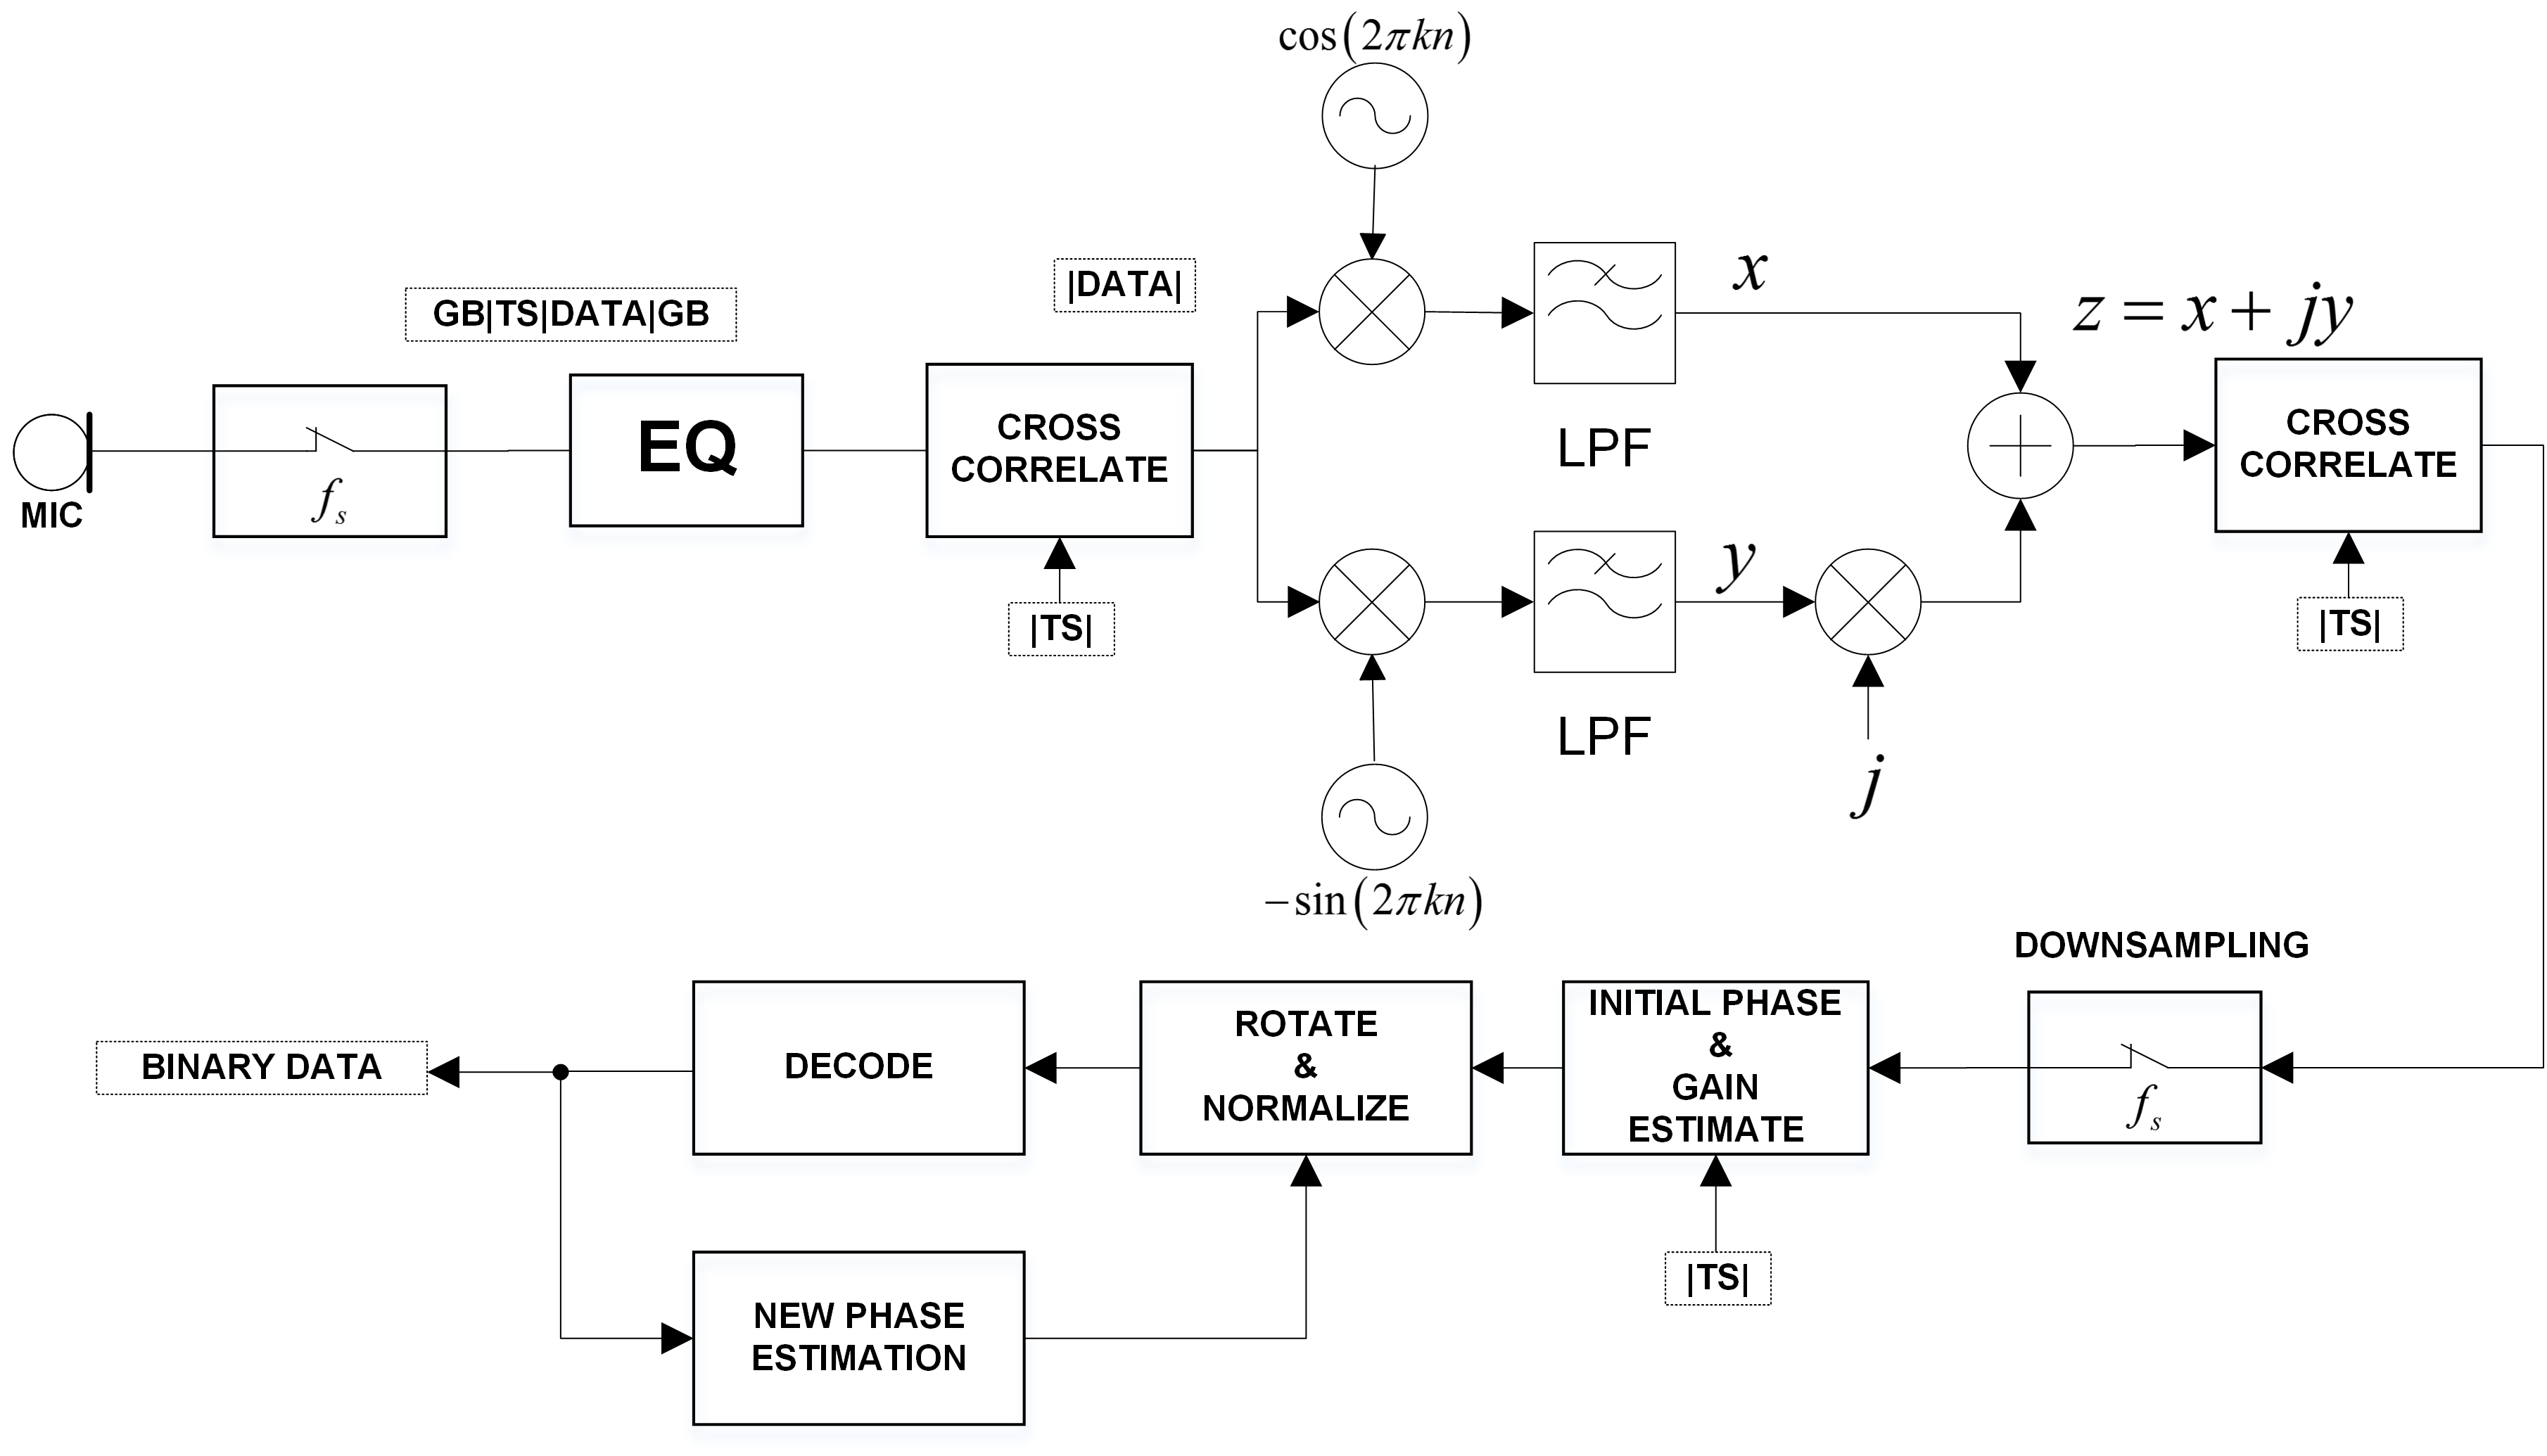
\includegraphics[width=1\textwidth]{rcvrSchem.png}
    \caption[Schematic of M-QAM Receiver]{Schematic of M-QAM Receiver.}
    \label{fig:SchemMQAMrecvr}
\end{figure}


% from the $.log$ file 
We will now describe the demodulation process. The received signal is filtered with the equaliser (EQ). The chosen equaliser is a parametric IIR filter which coefficients are computed according to the process that will be detailed in section \ref{sec:EQdesign}.The received constellations before, and after applying the equaliser are depicted in \ref{fig:RcvdQAMsignal}.
 

 \begin{figure}[H]
 \centering
 \begin{subfigure}{.4\textwidth}
   \centering
   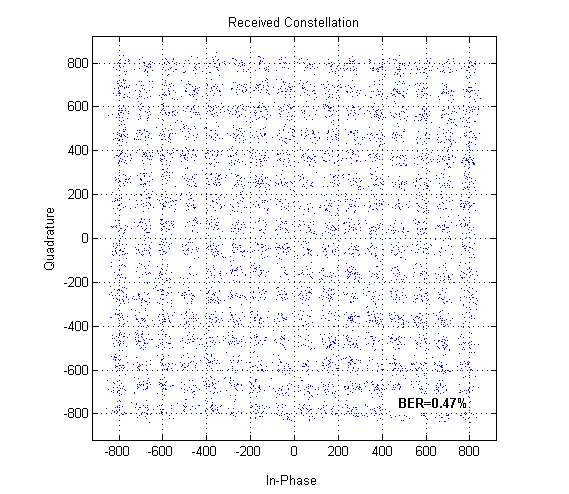
\includegraphics[width=\textwidth]{rcvdNOEQ.png}
   \subcaption{Constellation after phase\\ estimation without equaliser.}
   \label{fig:ConstBeforeFilt}
    \end{subfigure}%
 \begin{subfigure}{.4\textwidth}
   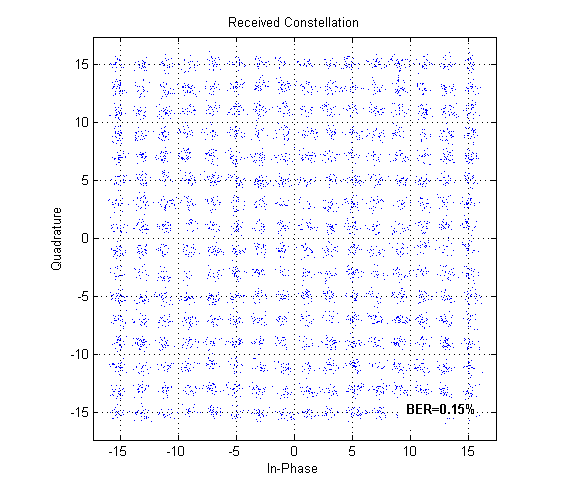
\includegraphics[width=\textwidth]{rcvdEQ.png}
       \subcaption{Constellation after phase\\ estimation with equaliser.}
     \label{fig:ConstAfterFilt}
    \end{subfigure}
 \caption[Received 64-QAM constellation and the effect of the equaliser]{Received 64-QAM constellation and the effect of the equaliser. There is a clear improvement in the BER when using the filter.}
    \label{fig:RcvdQAMsignal}
 \end{figure} 

 
 After the equalisation process, the beginning of the transmission must be found and a sample-level cross-correlation between the modulated training sequence and the received sequence is computed. Then, the lag $k$, which leads to the maximum value in the cross-correlation, is computed and considered as the beginning  of the training sequence. The samples are then multiplied by the carriers depicted in figure \ref{fig:SchemMQAMrecvr}. The next step is low-pass filter the resulting samples. For this stage, we use an order $N=14$ linear phase FIR filter modelled with the window method. The optimal parameters are obtained iteratively based on the resulting performance. 
 
At this point, up sampled received symbols must be down sampled. The optimal choice for the sampling instants is estimated using a symbol-level cross-correlation, taking into account the received symbols and the training sequence symbols, as referred in section \ref{subsec:MQAMsynch}. 

The consequent steps consist on the process blocks of phase and channel gain estimation. The latter parameter depend on the volume of the transmitter and is assumed to be constant during the whole transmission (even though there are implemented algorithms to keep track of it). The initial phase rotation is estimated according to the algorithm mentioned in section \ref{subsec:MQAMsynch}.

To make the system robust to longer transmissions(larger file sizes), the method mentioned in \ref{subsec:Phase rotation} is used to keep track of the Doppler shift.  It consists on dividing the set of symbols into smaller subsets, to which the Maximum Likelihood (ML) decision is applied, subsequently the new phase rotation is estimated. This new phase estimation block is used to rotate the symbols in the following blocks. This algorithm assumes that the  decoded symbol is correct and the added noise is zero-mean. It is important to choose a block with adequate length. It should not be too large neither too small\footnote{If the block is too large, there is a risk of error in the decoding due to the rotation, leading to a wrong decision feedback. If the block is too small, the assumption that the noise is zero-mean might not be accurate.}.   Denoting $t$ as the interval of time in which the Doppler shift does not majorly influence the decision, the size of the block in number of symbols is given by:
\begin{equation}
B_{sym} = \frac{t}{T_s} = \frac{t\times f_s}{n_{sym}}
\end{equation}

After processing all the blocks, the decisions from each one of those blocks can be merged together and compared with the transmitted data to compute the BER. 

\subsubsection{Optimization}

There are several parameters that can be adjusted and will influence the performance of the system:
\begin{description}
\item[\bf EQ.] Equaliser. The gain, bandwidth and central frequency of the equaliser will have a major impact in the decoding.
\item[\bf LPF.] Low-pass filter. The cut-off frequency, the order of the filter and the used window should be carefully chosen in order to suppress undesired spectral components. 
\item[\bf $t$.] Block length for decoding. The variable $t$ denotes the estimated interval of time in which the Doppler shift does not majorly influence on the decision. 
\end{description}


\section{OFDM System}

For the implementation of the OFDM system, the block schematic in figure \ref{fig:ofdmtransceiver} was used as a reference. On the transmitter side that are a set of parameters that need to be defined:
\begin{itemize}
\item $N_{FFT}$; The size of the FFT that is to be used. This parameter should not be neither too large or neither too small and it should be a power of two\footnote{A too small  $N_{FFT}$ will lead to more overhead (due to P and S) and will hence reduce the rate. A too large $N_{FFT}$ will take more time to compute and the sub-carrier spacing will decrease which leads to increased ICI.}.
%
\item    $f_c$; The carrier frequency should be chosen so that the bandwidth of the signal remains inside the available bandwidth.
\item $ P,S$; Cyclic prefix and suffix lengths are set according to the channel response.
 \item $N_c$; The number of active subcarriers will define the utilized bandwidth according to equation \ref{eq:OFDMbw}, and it is a very important parameter for the performance of the system. 

\end{itemize}

After these parameters are set and the size of the constellation is defined, the modulation algorithm takes place. Guard bits, training sequence and data to be transmitted are first merged and then mapped into the complex constellation. In the implementation, there is an option to insert pilots after each $N_{interval}$ transmitted bits. These pilots are used to reestimate the channel. However, apart from the frequency offset, the channel is time-invariant and hence, better performance is obtained when these reference symbols are not used. Then, the symbols are input into the OFDM modulation function. There are $N_{FFT}$ subcarriers for each OFDM symbol, but only $N_c$ are used (the number of virtual subcarriers is $N_{FFT}-N_c$). Each of these blocks of size $N_c$ is split into two, and saved into the corners of a buffer of size $N_{FFT}$, as depicted in figure \ref{}. Then, the FFT of each of these blocks is computed and cyclic prefix and suffix are added, according to the mentioned in section \ref{} (this operation is shown in figure \ref{}). The resulting signal is then upconverted using a complex exponential of frequency  $f_c$ and its real part is transmitted.   

On the receiver side there is no need for equaliser, since OFDM is being used. An high pass filter might be used to filter the low components of the noise. The received signal is then cross-correlated with the training sequence and the guard bands and silent parts are cropped. Afterwards, down conversion is performed, using the carrier frequency exponential and, subsequently, the cyclic prefixes and suffixes removed. To retrieve the complex transmitted symbols, the resulting samples are divided into blocks of $N_{FFT}$ size and FFT is applied. The received training sequence symbols are compared with the transmitted and the phase and gain estimations are computed for each of the subcarrier frequencies. An example of the outcome of these estimations is depicted in figure \ref{}. It is possible to verify the non-linearities of the channel in both amplitude and phases. Since it is known in which subcarrier the symbols are transmitted, the corresponding phase and amplitude corrections are applied accordingly. The frequency offset correction algorithm is the same as the one used in the complex baseband implementation, and is explained in section \ref{}. An example of the received constellations in OFDM before and after correction is depicted in figure \ref{}.

\section{Channel Coding}
\label{sec:ChanCodTests}
Since our system is implemented purely in software, we have to use a coding scheme that does not introduce too much delay and heavy processing to the phone. On the other hand, our goal is to implement an application capable to transmit digital files, thereby we should guarantee a transmission with zero errors or being capable to correct all of them. Such task is not completely straightforward, since the BER will depend in many different factors that shall be analysed separately to measure the effect in the transmitted data. 
The chosen modulation scheme for our performance analysis test is 256-QAM. We selected such configuration, since it was not possible to get an error free transmission with this setup. The first step, is to compare the performance of our MATLAB implementation with the theoretical performance of uncoded 256-QAM. Using MATLAB's embedded function \texttt{berawgn}\footnote{Computed according to equation \ref{eq:mqamBER} from section \ref{sec:MQAMperf}.}, and simulating an AWGN channel, we see in figure \ref{fig:MQAMperf} that the achieved performance with our implementation approximates the theoretical one.


 \begin{figure}[H]
  \centering
    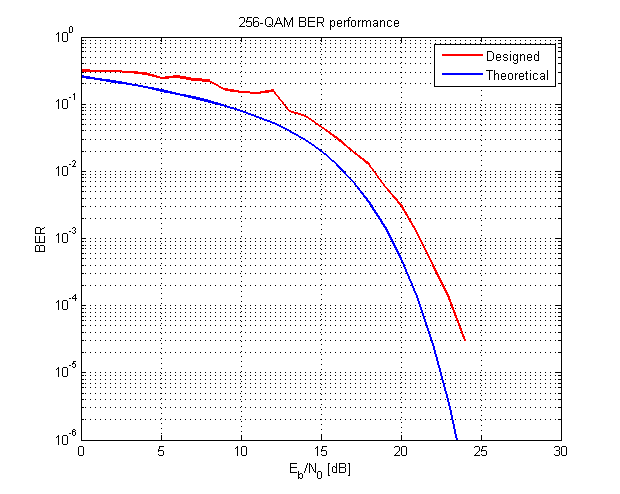
\includegraphics[width=0.5\textwidth]{BERuncoded.png}
    \caption[Performance of 256-QAM system]{Performance of 256-QAM system compared with the theoretical.}
    \label{fig:MQAMperf}
\end{figure}

From this point, we can introduce coding into our simulation and measure the performance for different code rates. The suggested FEC implementation is a variable rate convolutional encoder with maximum free distance (according to \cite{Proakis}) at the following code rates: $1/2$, $2/3$,$3/4$, and $4/5$. The used generator polynomials are $[15,17]$, $[27,75,72]$, $[13,25,61,47]$, and $[237,274,156,255,337]$, respectively. 
The simulation shows that for the theoretical case, one can reduce the number of errors significantly. Despite of this, we could not correct all the errors in the real channel, even with using the lowest code rate ($1/2 $). In addition, using 256-QAM with a coding scheme would end up getting us practically the same throughput compared to the case of uncoded 64-QAM. The results can be summarised in table \ref{table:Rates}.


\textcolor{red}{Add performance results.}
\begin{table} [h]
\centering
\begin{tabular}{lcccc} 
\hline
\bf{Scheme} 				       & \bf{Raw data rate}\textnormal{[kbps]}    & \bf{Real data rate}\textnormal{[kbps]} & ${{\text{\bf E}}_{\text{\bf b}}}/{{\text{\bf N}}_{\text{\bf 0}}}$ [dB] &\bf{BER} \\
\hline
\emph{256-QAM, NO FEC}           & 44.10            & 35.46      & 21        & 1.397$\times 10^{-4}$      \\
\emph{256-QAM, FEC:$1/2$}        & 44.10            & 4          & 6       & 1.397$\times 10^{-4}$                      \\
\emph{256-QAM, FEC:$3/4$}        & 44.10            & 4          & 4      & 1.397$\times 10^{-4}$\\
\hline
\emph{64-QAM, NO FEC}            & 33.08           & 27.96       & 7     & 1.397$\times 10^{-4}$  \\
\hline
\end{tabular}
\caption[Performance of different modulation/coding schemes]{Performance of different modulation/coding schemes.}
\label{table:Rates}
\end{table}




\section{Channel Equalisation and filter design}
\label{sec:EQdesign}
In order to characterise the channel and determine the best possible way to deal with the distortion that is present, we estimated the channel transfer function with a non-parametric correlation method that got us $k=45$ taps of a FIR model with order $N=k-1=44$. Such process was done using MATLAB's function \texttt{impulseest}, which is based on a least-squares algorithm to obtain the coefficients. The resulting transfer function is plotted in figure \ref{fig:FIRtf}. 
 
 
\begin{figure}[h]
  \centering
    \includegraphics[width=1\textwidth]{FIRChanRespose.png}
    \caption[Estimated least-squares FIR model for the channel transfer function]{Estimated least-squares FIR model of the channel transfer function. The filter order is $N=44$.}
    \label{fig:FIRtf}
\end{figure}

An inverse optimal equaliser filter using this method is not stable, for this reason, the filter has to be constructed based on a parametrical IIR model. The function \texttt{fdesign.parameq} constructs a Chebyshev Type I peak filter (figure   \ref{fig:IIRpeak}) with the following transfer function:

\begin{equation}
H\left( z \right) = \frac{{{b_0} + {b_1}{z^{ - 1}} + {b_2}{z^{ - 2}}}}{{1 + {a_1}{z^{ - 1}} + {a_2}{z^{ - 2}}}}
\end{equation}

The filter main design parameters are central frequency, passband bandwidth, reference gain, and passband gain. The reconstructed channel based on these approach is depicted in figure \ref{fig:cascadefilter}. Once the parameters are defined we obtain the coefficients from MATLAB and run an iterative process to optimize the filter to perform well in all the phones.

\begin{figure}[H]
\centering
\begin{subfigure}[H]{.8\textwidth}
  \centering
  \includegraphics[width=1\linewidth]{peakFilter.png}
  \caption{IIR peak filter.}
  \label{fig:IIRpeak}
  \quad
\end{subfigure}%
\quad
\begin{subfigure}[H]{.8\textwidth}
  \centering
  \includegraphics[width=1\linewidth]{reconstChan.png}
  \caption{Cascaded channel after filtering.}
  \label{fig:cascadefilter}
\end{subfigure}
\caption[Channel reconstruction using the IIR peak filter]{Channel reconstruction using the IIR peak filter.}
   \label{fig:chanReconstruction}
    \end{figure}

% % % % % % % % % % % % % % % % % % % % % % % % % % % % % % % % % % % % % % % % % % % % % % % % % % % % % % % % %
% % % % % % % % % % % % % % % % % % % % % % % % % % % % % % % % % % % % % % % % % % % % % % % % % % % % % % % % %


\chapter{Results and discussion}
We tested several modulations schemes modulating and demodulating random binary sequences, first with MATLAB (off-line mode), and then with the phones with the provided Android Framework (on-line mode). 

In the offline mode, transmitter and receiver processing is done solely in MATLAB. The transmitted samples are sent to the phone in a file (\texttt{.dat}) of $shorts$, read by the application and delivered to the sound card buffer to be played. On the receiver side, there is a recording application which stores the audio samples in a \texttt{.log} file. The file is then transferred to the computer and the samples extracted to be processed. 

MATLAB is a powerful tool for simulation due to its computation power and adaptability and was, hence, chosen to find the optimal algorithms/methods/parameters for the implementation of a robust system. Once found, these methods can, with a little effort, be translated into Java. If done correctly this translation should not cause the final results to be much different in both real-time and off-line systems. 

\textcolor{red}{Write about major differences in algorithm implementation.}%
\section{Binary FSK}
Our first and basic test was to generate a random sequence and transmit it with binary FSK throughout the channel. As discussed in section \ref{sec:FSKdemod}, we used the Goertzel algorithm to decode the received modulated signal with generally good results. The maximum bit rate was about 1.5 kbps. We end up using binary shift keying only to modulate the training sequence in the 4-FSK scheme that will be described next. 

\begin{figure}[H]
  \centering
    \includegraphics[width=0.5\textwidth]{demo.png}
    \caption[Add caption]{Add plots}
    \label{fig:4FSKplots}
\end{figure}

\section{4-FSK}

 In the implementation, $n_{sym}= 35$ samples were used, resulting in a rate of $R=2.52$ kbps with no errors and without the use of any coding scheme. This value for the rate considers all the bits that were transmitted, including guard band and training sequence (of length 100 bits). Hence, the effective rate is lower than this value but still well above the basic requirements of 1 kbps. A section of the  transmitted/received samples and corresponding spectrum is depicted in figure \ref{fig:4FSKplots}, using rectangular and Hanning window.
 
\begin{figure}[H]
  \centering
    \includegraphics[width=0.5\textwidth]{demo.png}
    \caption[Add caption]{Add plots}
    \label{fig:4FSKplots}
\end{figure}
 
 
\section{4-FSK and FDM}
In order to improve the rate and to exploit all the available bandwidth, a FDM (frequency division multiplexing) system is used. The idea is to replicate the 4-FSK transmission in the previous section $N_r$ times until all available bandwidth is used. Replicating the system $N_r=7$ times, it was still possible to obtain a reliable transmission. However, it was necessary to increase $n_{sym}$ to $102$ samples, resulting in a rate of:

$$ R = \frac{N_r\times log_2(4)}{n_{sym}}\times f_s = 7 \times \frac{2}{102}\times f_s = 6052 \text{ bps}$$

This value more than doubles the value achieved with the single 4FSK system. A gaussian window was used in order to modulate the samples. The resulting signals and power spectrum densities  are depicted in Fig. \ref{fig:FDMplots}.

\begin{figure}[H]
  \centering
    \includegraphics[width=0.5\textwidth]{demo.png}
    \caption[Spectrum plots of the FDM-FSK signal.]{Spectrum plots of the FDM-FSK signal. }
    \label{fig:FDMplots}
\end{figure}


\section{M-QAM}

The 64 MQAM framework is tested by sending different types of files of different sizes
and making sure the received file is not corruupt by using the check sum method described in section. In Fig. \ref{fig:20140508Transmittermoreexample} a screenshot
is provided of an example where a text file (more.txt) of size 10kB (9707 bytes) is sent. The functions at the receiver are
timed in order to make sure that the data rate requirement is achieved. The checksum number is displayed in both
the transmitter and receiver. If these numbers are the same the file transfer is successful.

\begin{figure}[H]
 \centering
 \begin{subfigure}{.5\textwidth}
 \centering
    \includegraphics[width=0.8\textwidth]{20140508Receivermoreexample.png}
    \subcaption{Receiver}
    \label{fig:20140508Receivermoreexample}
    \end{subfigure}%
 \begin{subfigure}{.5\textwidth}
  	 \centering
      \includegraphics[width=0.8\textwidth]{20140508Transmittermoreexample.png}
      \subcaption{Transmitter}
      \label{fig:20140508Transmittermoreexample}
   \end{subfigure}
\caption[Screenshots of receiver and transmitter in M-QAM application]{Screenshots of receiver and transmitter in M-QAM application}
 \end{figure} 

\section{OFDM}

\section{M-FSK}




% % % % % % % % % % % % % % % % % % % % % % % % % % % % % % % % % % % 
% % % % % % % % % % % % % % % % % % % % % % % % % % % % % % % % % % %
\chapter{Conclusion}


\begin{thebibliography}{1}

\bibitem{Madhow}
Madhow U., \emph{Fundamentals of Digital Communication}, Cambridge , 2008.

\bibitem{Proakis}
Proakis J. ,Salehi Masoud, \emph{Digital Communications}, McGraw-Hill , 2008.

\bibitem{ASKDemGaza}
Abu M., \href{http://site.iugaza.edu.ps/mabufoul/files/2010/09/Experiment-5.pdf}
{\emph{ASK demodulator Lab Experiment}},
Islamic University of Gaza, retrieved in April 2014.


\bibitem{DigModTech}
Sa-nguankotchakorn T. , \href{http://www.tc.ait.ac.th/faculty/teerapat/AT77.11_Digital\%20Modulation\%20Techniques/III.Frequency_Shift_Keying.pdf}{\emph{Frequency Shift Keying Lecture Slides}}, Asian Institute of Technology, retrieved in April 2014.


\bibitem{DigCommLec}
Okechukwu C. Ugweje, \href{ugweje/web/Courses/Ee549/Handout/EE549F01Lecture37.pdf}{\emph{Frequency Shift Keying, Lecture Slides}},  University of Akron, retrieved in April 2014.


\bibitem{XiongDigModTech}
Xiong F., \emph{Digital Modulation Techniques}, Artech House, 2006.

\bibitem{gold}
Shembil S., \emph{M-Ary FSK with Orthogonal Pulse Envelopes and its Noncoherent Detection}, IJECS-IJENS, Vol. 10, No.06, Issued December 2010, pp. 103-106.

\bibitem{GoertzelPaper}
Sysel and Rajmic, \emph{Goertzel algorithm generalized to non-integer multiples of fundamental frequency}, EURASIP Journal on Advances in Signal Processing, 2012, 2012:56.

\bibitem{ProjectEQ2310}
Project Assignment EQ2310 Digital Communications, \emph{Analysis and Simulation of a QPSK System}, KTH, 2013.

\bibitem{EQ2440ProjectDescription}
Project Description EQ2320 PROJECT IN WIRELESS COMMUNICATION, \emph{Project \#1: In-flight file-transfer using 3-mm cable}, KTH, 2014.

\bibitem{HaykinBook}
Haykin S., \emph{Digital Communication Systems}, John Wiley \& Sons, Inc., 2014.

\bibitem{CarrierSynchPaper}
Dick D., Harris F., and Rice M., \emph{FPGA Implementation of Carrier Synchronization for QAM Receivers}, Journal of VLSI Signal Processing 36, 57-71, 2004.

\bibitem{NI QAM white-paper}
National Instruments, (2012),\href{http://www.ni.com/white-paper/3896/en/}{\emph{Quadrature Amplitude Modulation (QAM)[White paper]}}, retrieved in May 2014.

\bibitem{Agilent IQ paper}
Agilent Technologies,(2013) \href{http://wireless.agilent.com/wireless/helpfiles/89600B/WebHelp/subsystems/digdemod/content/digdemod_para_interact_iqgainimb_quadskewerr.htm}{\emph{IQ Gain Imbalance and Quadrature Skew Error Data Interaction (Digital Demod)[9600 VSA Software - Product Documentation]}}, retrieved in May 2014.

\bibitem{BER-QAM paper}
Yoon D., Cho K., and Lee J., \emph{Bit Error Probability of M-ary Quadrature Amplitude Modulation}, Vehicular Technology Conference, 2000. IEEE-VTS Fall VTC 2000. 52nd , vol.5, no., pp.2422,2427 vol.5, 2000.
\bibitem{DSPDiniz}
Diniz P., Da Silva E., Netto S., \emph{Digital Signal Processing: System Analysis and Design}, Cambridge University Press, 2010.

\bibitem{SklarBook}
Sklar B., \emph{Digital Communications Fundamentals and Applications}, Prentice Hall, 2001.


\bibitem{FFTJavaRef} 
Robert Sedgewick and Kevin Wayne,
\href{http://introcs.cs.princeton.edu/java/97data/FFT.java.html}{\emph{FFT.java}},  Princeton
Copyright © 2000–2011

\bibitem{ComplexJavaRef} 
Robert Sedgewick and Kevin Wayne,
\href{http://introcs.cs.princeton.edu/java/97data/Complex.java.html}{\emph{Complex.java}},  Princeton
Copyright © 2000–2011

\bibitem{Checksumref1} 
D.  Borman, 
Cray Research, 
C. Partridge, 
R.  Braden, 
\href{http://introcs.cs.princeton.edu/java/97data/Complex.java.html}{\emph{Computing the Internet checksum}}, BBN Laboratories, 
September 1988





%% Slides & handouts



\end{thebibliography}


\end{document}